\documentclass[12pt]{book}
\usepackage[margin=1in]{geometry}

\usepackage{tikz}
\usepackage{float}
\usepackage{xcolor}
\usepackage{caption}
\usepackage{chemfig}
\usepackage{gensymb}
\usepackage{listings}
\usepackage{setspace}
\usepackage{pgfplots}
\usepackage{textcomp}
\usepackage{graphicx}
\usepackage{booktabs}
\usepackage{multirow}
\usepackage{hyperref}
\usepackage{csquotes}
\usepackage{amsfonts}
\usepackage{adjustbox}
\usepackage{subcaption}
\usepackage[T1]{fontenc}
\usepackage[utf8]{inputenc}
\usepackage[english]{babel}
\usepackage{amsmath, amssymb}
\usepackage{tabularx, ragged2e}

\usepackage[numbers]{natbib}
\bibliographystyle{plain}
\usetikzlibrary{patterns}
\onehalfspacing

\definecolor{backcolour}{rgb}{0.95,0.95,0.92}
\definecolor{gridgrey}{RGB}{176,176,176}
\definecolor{legendgray}{RGB}{204,204,204}
\definecolor{steelblue}{RGB}{31,119,180}
\definecolor{darkorange}{RGB}{255,127,14}

\hypersetup{
  colorlinks=true,
  linkcolor=blue,
  citecolor=blue,
  filecolor=blue,
  urlcolor=blue
}
\lstset{
  language=Python,
  basicstyle=\ttfamily\footnotesize, % Small font size
  numbers=none, % Line numbers on the left
  stepnumber=1, % Line number step
  tabsize=2, % Tab size
  breaklines=true, % Allow line breaks
  showstringspaces=false,
  backgroundcolor=\color{backcolour},
  keywordstyle=\color{blue},
  stringstyle=\color{red},
  commentstyle=\color{green},
  captionpos=b,
  framextopmargin=2em,
  framexleftmargin=1em,
  framexrightmargin=1em,
  framexbottommargin=2em,
}

\setcounter{secnumdepth}{3}
\setcounter{tocdepth}{3}

\newcommand{\pseudo}{\ensuremath{\Psi}} % Pseudouridine symbol for RNA research

\begin{document}
  \title{Pseudouridine Modification Detection in RNA}
  \author{Muhammad Arish Sultan Khan}

  \maketitle

% Table of Contents
  \tableofcontents
  \newpage

% Chapter Sections

  \chapter{Introduction}
  \label{ch:introduction}

  RNA modifications have emerged as pivotal regulators of gene expression and cellular function.
Among these modifications, pseudouridine (\pseudo) stands out as the most abundant and one of the earliest discovered nucleoside modifications in RNA~\cite{charette_pseudouridine_2000}.
This research focuses on developing computational models using machine learning (ML) and deep learning (DL) algorithms to predict pseudouridine sites within RNA sequences.
By accurately identifying these sites, we aim to enhance the understanding of pseudouridylation's role in biology and its implications in human diseases, thereby facilitating the development of novel diagnostic and therapeutic strategies.


\section{Overview}\label{sec:overview}
  Pseudouridine (\pseudo), a modified nucleoside, is the 5-ribosyl isomer of uridine and is the most common RNA modification across various RNA types.
  It was first discovered in transfer RNA (tRNA), but its presence has been identified in ribosomal RNA (rRNA), small nuclear RNA (snRNA), and messenger RNA (mRNA)~\cite{cohn_nucleoside-5-phosphates_1951}.

  Pseudouridine formation occurs through a process called pseudouridylation, catalyzed by enzymes known as pseudouridine synthases.
  During this modification, the nitrogen-carbon (N\textminus{C}) glycosidic bond of uridine is rearranged into a carbon-carbon (C\textminus{C}) glycosidic bond.
  This modification changes the structural properties of RNA, allowing pseudouridine to participate in enhanced hydrogen bonding and increase RNA stability~\cite{charette_pseudouridine_2000}.

  The key structural difference between uridine and pseudouridine lies in this glycosidic bond.
  While uridine has a nitrogen atom at position 1 connected to the ribose sugar, pseudouridine has a carbon atom at position 5 linked to the ribose, which provides additional hydrogen bonding capabilities.
  This structural change reinforces the RNA backbone and contributes to the overall stabilization of RNA molecules, making pseudouridine important in maintaining RNA function and conformation~\cite{ge_rna_2013}.

  \begin{figure}[h!]
    \centering
    \chemname{
      \chemfig[cram width=2pt]{HO?<[:-60](-[6]OH)-[,,,,line width=2pt](-[6]OH)>[:60]-[:150, 1.1]O?}
    }{Uridine}

    \chemname{
      \chemfig{*6((=O)-N-(*5(-N=-N(-H)-))=-(=O)-N(-H)-)}
    }{Pseudouridine}

    \caption{Chemical structure of uridine and pseudouridine with numbering of selected atoms.}
    \label{fig:structure-pseudouridine}
  \end{figure}

  \textbf{Figure~\ref{fig:structure-pseudouridine}} provides a comparison of the structures of uridine and pseudouridine, highlighting the key difference in glycosidic bond placement.

  \section{Importance of Pseudouridine}\label{sec:importance-of-pseudouridine}
  \subsection*{Biological Significance}
    Pseudouridine is formed through the isomerization of uridine residues in RNA, a reaction catalyzed by pseudouridine synthases \cite{carlile_pseudouridine_2014}.
    This modification plays several important roles:

    \begin{itemize}
      \item \textbf{Structural Stability}: The conversion of uridine to pseudouridine introduces a C–C glycosidic bond, enhancing base stacking and stabilizing RNA secondary and tertiary structures~\cite{ge_rna_2013}.
      \item \textbf{RNA Function}: Pseudouridine is widely found in transfer RNA (tRNA), ribosomal RNA (rRNA), small nuclear RNA (snRNA), and messenger RNA (mRNA). In tRNA and rRNA, pseudouridylation maintains proper folding and function, crucial for accurate protein synthesis and ribosome assembly~\cite{schwartz_transcriptome-wide_2014}.
      \item \textbf{Pre-mRNA Splicing}: In snRNA, pseudouridylation is essential for the proper functioning of the spliceosome, influencing pre-mRNA splicing and gene expression regulation \cite{karijolich_converting_2011}.
      \item \textbf{Regulation of mRNA Translation}: Recent studies suggest pseudouridine in mRNA plays a role in regulating translation and cellular stress responses~\cite{carlile_pseudouridine_2014}.
    \end{itemize}

  \subsection*{Clinical Impacts}
    Aberrant pseudouridylation has been implicated in various human diseases. Key clinical impacts include:

    \begin{itemize}
      \item \textbf{Cancer:} Dysregulated pseudouridine synthase activity may promote tumorigenesis by altering the translation of oncogenes or tumor suppressor genes \cite{ramamurthy2020role}.
      \item \textbf{Genetic Disorders:} Mutations in pseudouridine synthase genes have been linked to disorders like dyskeratosis congenita, which affects telomere maintenance and leads to premature aging \cite{mason2008dyskeratosis}.
      \item \textbf{Neurological Diseases:} Altered pseudouridylation patterns are implicated in neurodevelopmental and neurodegenerative disorders \cite{havelund2017pseudouridine}.
      \item \textbf{Viral Infections:} Viruses may exploit host pseudouridylation mechanisms to enhance viral RNA stability and evade immune responses \cite{karijolich2015viral}.
    \end{itemize}

  \section{Pseudouridine Detection Techniques}\label{sec:pseudouridine-detection-techniques}
  \subsection*{Chemical Detection}

    Detecting pseudouridine (\pseudo) in RNA is challenging due to its subtle structural differences from uridine.
    Several traditional experimental techniques require specialized equipment and manual labor, making them resource-intensive.
    These methods include:

    \begin{itemize}
      \item \textbf{High-Performance Liquid Chromatography (HPLC)}: Used for separation and identification of nucleoside modifications, including pseudouridine, but it is labor-intensive and unsuitable for large-scale studies~\cite{gehrke_quantitative_1982}.
      \item \textbf{Mass Spectrometry (MS)}: Provides highly accurate detection but requires complex protocols and specialized equipment, limiting its scalability for high-throughput studies~\cite{de_hoffmann_mass_2011}.
      \item \textbf{Next-Generation Sequencing-Based Methods}: Techniques such as Pseudo-seq and $\Psi$-seq use chemical derivatization to map pseudouridine across the transcriptome, but these methods are also complex and resource-intensive~\cite{carlile_pseudo-seq_2015}.
    \end{itemize}

  \subsection*{Computational Prediction}
    Machine learning (ML) and deep learning (DL) have become integral tools in bioinformatics, offering scalable and cost-effective methods for analyzing complex biological data.
    These computational approaches can process large datasets to identify patterns and make predictions that are impractical with traditional techniques.

    Key advantages of ML-based methods in bioinformatics include:

    \begin{itemize}
      \item \textbf{High-Throughput Data Analysis}: ML algorithms can handle vast amounts of biological data, enabling the analysis of genomic, transcriptomic, proteomic, and metabolomic datasets.
      \item They can identify patterns and associations that are not readily apparent, facilitating discoveries in areas such as gene expression profiling and variant detection~\cite{libbrecht_machine_2015}.

      \item \textbf{Feature Extraction and Predictive Modeling}: ML models can learn complex relationships by extracting relevant features and building predictive models.
      \item In bioinformatics, this allows for accurate prediction of protein structures, gene functions, and disease associations~\cite{chicco_machine_2020}.

      \item \textbf{Integration with Experimental Data}: Computational predictions complement experimental approaches by providing insights that guide experimental design.
      \item For example, ML models can prioritize candidate genes or pathways for further investigation, saving resources and focusing efforts where validation is most needed~\cite{larranaga_machine_2006}.

      \item \textbf{Scalability and Flexibility}: ML-based approaches are highly scalable and adaptable to various biological problems and datasets.
      \item They can be applied across different organisms and conditions, which is essential for studying complex biological systems and diseases~\cite{min_deep_2016}.

      \item \textbf{Continuous Improvement}: ML models can be continually refined as new data become available, improving their predictive accuracy over time.
      \item This iterative learning process is crucial in bioinformatics, where data is constantly being generated~\cite{esteva_guide_2019}.
    \end{itemize}

  \section{Significance of Computational Techniques}\label{sec:significance-of-computational-techniques}
  Although clinical and experimental approaches, such as High-Performance Liquid Chromatography (HPLC), Mass Spectrometry (MS), and Next-Generation Sequencing (NGS)-based methods, are considered the gold standard for detecting pseudouridine, these techniques are often labor-intensive, costly, and time-consuming.
  Each of these methods requires specialized equipment, expert personnel, and careful handling of RNA samples, making them impractical for high-throughput or large-scale studies.

  \begin{itemize}
    \item \textbf{HPLC}: requires precise calibration and laborious sample preparation, making it both time- and labor-intensive, especially when dealing with multiple samples.
    \item \textbf{Disease Mechanisms}: provides highly accurate results, but the equipment is expensive, and the sample processing steps are complicated.
    This limits its accessibility for routine use or large-scale studies.
    \item \textbf{Novel Therapeutic Targets}: such as Pseudo-seq and $\Psi$-seq offer a transcriptome-wide mapping of pseudouridine but require chemical derivatization and expensive reagents, adding to the cost and time demands of these methods.
  \end{itemize}

  While these clinical approaches offer high accuracy, they are not scalable for genome-wide studies or large datasets due to their resource-intensive nature.

  \subsection*{Advantages of Computational Techniques}
    In contrast, computational techniques-particularly those leveraging machine learning (ML)-provide a highly scalable and cost-effective solution for pseudouridine site prediction.
    Despite their computational limitations in precision compared to clinical methods, ML-based approaches offer several advantages:

    \begin{itemize}
      \item \textbf{Efficiency and Scalability}: Computational models can analyze large RNA sequence datasets simultaneously.
      For instance, a single ML model trained on known pseudouridine sites can predict potential sites across thousands of RNA sequences in a fraction of the time it would take to manually process these samples in a lab.
      This scalability is crucial for genome-wide studies, where clinical methods would be impractical due to time and cost constraints.
      \item \textbf{Cost-Effectiveness}: While clinical methods require expensive reagents, specialized instruments, and expert operators, computational methods require only the initial setup of data and algorithms, making them far more cost-effective for large-scale studies.
      Once a computational model is built, it can be applied to any number of RNA sequences without significant additional cost.
      \item \textbf{Rapid Hypothesis Generation}: ML models allow researchers to generate predictions quickly, providing insights that can guide experimental validation.
      Instead of laboriously testing every RNA sequence experimentally, researchers can use ML predictions to prioritize sequences for clinical validation, significantly reducing the number of experiments needed.
      This synergy between computational and clinical approaches enhances research efficiency.
      \item \textbf{Simultaneous Analysis of Multiple Conditions}: ML models can be trained to detect patterns across diverse biological conditions (e.g., different cell types, stress conditions, or disease states).
      In contrast, traditional clinical methods would require running individual experiments for each condition, making it impractical to study pseudouridylation under multiple scenarios at once.
    \end{itemize}

    While clinical techniques are undeniably more accurate in detecting pseudouridine, computational methods offer a complementary approach that accelerates the discovery process, enabling rapid analysis of large datasets.
    By integrating computational predictions with experimental validation, researchers can efficiently explore pseudouridylation across different organisms, tissues, and disease contexts.
    In the next section we will discuss some of the available models that try to solve this problem to some extent in their own novel ways.

  \chapter{Related Work}\label{ch:related-work}
  In this section, we summarize the methodologies and findings of various studies related to the prediction of pseudouridine sites in RNA sequences.
  Each study is described in terms of its encoding schemes, feature selection methods, machine learning algorithms, and the accuracy or performance metrics achieved.
  Finally, we present a comparative analysis of the studies in a summary table.


  \section{Past Studies}\label{sec:past-studies}

    \subsection*{iRNA-PseU \cite{chen_irna-pseu_nodate}}\label{subsec:iRNA-PseU}
      This study employed a feature encoding scheme based on nucleotide chemical properties and nucleotide frequency.
      The chemical properties (e.g., purine/pyrimidine structure, amino/keto groups, and hydrogen bond strength) were encoded alongside nucleotide occurrence frequency.
      This aimed to capture the biological relevance of nucleotide sequences for pseudouridine site prediction.

      \begin{itemize}
        \item \textbf{Feature Encoding}: NCP~\ref{enc:NCP}, PseKNC~\ref{subsubsec:pseknc}.
        \item \textbf{Model}: SVM~\ref{model:SVM} with RBF kernel.
      \end{itemize}

    \subsection*{PseUI \cite{he_pseui_2018}}\label{subsec:PseUI}
      This study combined various feature encoding schemes, including nucleotide composition (NC), dinucleotide composition (DC), pseudo dinucleotide composition (pseDNC), position-specific nucleotide propensity (PSNP), and position-specific dinucleotide propensity (PSDP). It employed sequential forward feature selection (SFS) to create a compact, discriminative feature set for pseudouridine site prediction.

      \begin{itemize}
        \item \textbf{Feature Encoding}: NC~\ref{subsubsec:nc}, DNC~\ref{subsubsec:dnc}, PseDNC~\ref{enc:PseDNC}, PSNP~\ref{enc:PSNP}, PSDP~\ref{enc:PSDP}.
        \item \textbf{Feature Selection}: SFS~\ref{fs:SFS}, evaluated with MCC~\ref{subsec:mcc}.
        \item \textbf{Model}: SVM~\ref{model:SVM}, jackknife cross-validation.
      \end{itemize}

    \subsection*{XG-PseU \cite{liu_xg-pseu_2020}}\label{subsec:XG-PseU}
      This study used multiple feature encoding schemes, such as nucleotide composition (NC), dinucleotide composition (DNC), trinucleotide composition (TNC), nucleotide chemical properties (NCP), nucleotide density (ND), and one-hot encoding.
      A two-step feature selection (forward selection and increment feature selection) was employed for optimal performance in pseudouridine site prediction.

      \begin{itemize}
        \item \textbf{Feature Encoding}: NC~\ref{subsubsec:nc}, DNC~\ref{subsubsec:dnc}, TNC~\ref{subsubsec:tnc}, NCP~\ref{enc:NCP}, ND~\ref{subsec:nd}, one-hot~\ref{subsec:binary}.
        \item \textbf{Feature Selection}: Forward feature selection~\ref{fs:FFS} and IFS~\ref{fs:IFS}.
        \item \textbf{Model}: XGBoost~\ref{model:Xgboost}, 10-fold cross-validation.
      \end{itemize}

    \subsection*{iPseU-NCP \cite{nguyen-vo_ipseu-ncp_2019}}\label{subsec:ipseu_ncp}
      This study utilized Random Forest (RF) with nucleotide chemical property (NCP) encoding to represent the structural aspects of RNA sequences.
      Feature importance within the Random Forest model was used for feature selection.

      \begin{itemize}
        \item \textbf{Feature Encoding}: NCP~\ref{enc:NCP}, PseKNC~\ref{subsubsec:pseknc}, CKSNAP~\ref{subsubsec:pseknc}.
        \item \textbf{Feature Selection}: Feature importance ranking in RF
        \item \textbf{Model}: RF~\ref{model:RF}, grid search with 5-fold cross-validation.
      \end{itemize}

    \subsection*{PseU-FKeERF \cite{chen_fuzzy_2024}}\label{subsec:PseU-FKeERF}
      This study utilized fuzzy kernel evidence Random Forest (FKeERF) with several RNA sequence encoding schemes to identify pseudouridine sites.
      Fuzzy logic was used to expand the feature space, and feature selection was performed through fuzzy mean clustering and Gaussian fuzzy membership.

      \begin{itemize}
        \item \textbf{Feature Encoding}: Binary~\ref{subsec:binary}, PSTNPss~\ref{subsec:pstnpss}, NCP~\ref{enc:NCP}, PseKNC~\ref{subsubsec:pseknc}.
        \item \textbf{Feature Selection}: Fuzzy mean clustering and Gaussian fuzzy membership.
        \item \textbf{Model}: Fuzzy C-mean~\ref{model:fuzzy-c}, Evidential Random Forest~\ref{model:ERF}, cross-validation and independent tests.
      \end{itemize}


  \section{Comparison of Related Work}\label{sec:comparison-of-related-work}
    The table below presents a comparison of the encoding schemes, feature selection methods, machine learning algorithms, and performance metrics for the studies reviewed in this chapter.

    \begin{table}[h!]
      \centering
      \begin{tabular}{lcccc}
        \toprule
        \textbf{Study}                           & \textbf{Acc} (\%) & \textbf{MCC}    & \textbf{Sp} (\%) & \textbf{Sn} (\%) \\
        \midrule
        iRNA-PseU\cite{chen_irna-pseu_nodate}    & 60.40             & 0.21            & 59.80            & 61.01            \\
        PseUI\cite{he_pseui_2018}                & 64.24             & 0.2849          & 63.64            & 64.85            \\
        iPseU-CNN\cite{tahir_ipseu-cnn_nodate}   & 66.68             & 0.34            & 68.78            & 65.00            \\
        XG-PseU\cite{liu_xg-pseu_2020}           & 66.05             & 0.32            & 68.65            & 63.45            \\
        iPseU-NCP\cite{nguyen-vo_ipseu-ncp_2019} & 62.92             & 0.24            & 65.05            & 58.79            \\
        FKeERF\cite{chen_fuzzy_2024}             & 78.08 (91.99)     & 0.5644 (0.8504) & 78.66 (94.97)    & 77.62 (90.11)    \\
        \bottomrule
      \end{tabular}
      \caption{Comparison of all Past studies on Homo sapiens dataset}
      \label{tab:human_comp_table}
    \end{table}

    \begin{table}[h!]
      \centering
      \begin{tabular}{lcccc}
        \toprule
        \textbf{Study}                           & \textbf{Acc} (\%) & \textbf{MCC} & \textbf{Sp} (\%) & \textbf{Sn} (\%) \\
        \midrule
        iRNA-PseU\cite{chen_irna-pseu_nodate}    & 69.07             & 0.38         & 64.83            & 73.31            \\
        PseUI\cite{he_pseui_2018}                & 70.44             & 0.4103       & 66.31            & 74.58            \\
        iPseU-CNN\cite{tahir_ipseu-cnn_nodate}   & 71.81             & 0.44         & 69.11            & 74.79            \\
        XG-PseU\cite{liu_xg-pseu_2020}           & 71.10             & 0.43         & 76.30            & 65.92            \\
        iPseU-NCP\cite{nguyen-vo_ipseu-ncp_2019} & 71.82             & 0.44         & 76.27            & 67.37            \\
        FKeERF\cite{chen_fuzzy_2024}             & 77.87             & 0.5571       & 77.82            & 77.85            \\
        \bottomrule
      \end{tabular}
      \caption{Comparison of all Past studies on Mus musculus dataset}
      \label{tab:mouse_comp_table}
    \end{table}

    \begin{table}[h!]
      \centering
      \begin{tabular}{lcccc}
        \toprule
        \textbf{Study}                           & \textbf{Acc} (\%) & \textbf{MCC}    & \textbf{Sp} (\%) & \textbf{Sn} (\%) \\
        \midrule
        iRNA-PseU\cite{chen_irna-pseu_nodate}    & 64.49             & 0.29            & 64.33            & 64.65            \\
        PseUI\cite{he_pseui_2018}                & 65.92             & 0.3185          & 66.88            & 64.97            \\
        iPseU-CNN\cite{tahir_ipseu-cnn_nodate}   & 68.15             & 0.37            & 70.45            & 66.36            \\
        XG-PseU\cite{liu_xg-pseu_2020}           & 73.42             & 0.47            & 69.48            & 77.35            \\
        iPseU-NCP\cite{nguyen-vo_ipseu-ncp_2019} & 69.59             & 0.40            & 62.10            & 77.07            \\
        FKeERF\cite{chen_fuzzy_2024}             & 87.73 (94.5)      & 0.7589 (0.8898) & 89.98 (96.08)    & 86.08 (93.29)    \\
        \bottomrule
      \end{tabular}
      \caption{Comparison of all Past studies on Saccharomyces cerevisiae dataset}
      \label{tab:yeast_comp_table}
    \end{table}

  \chapter{Methodology}
  \label{ch:methodology}

  \input{sections/methodology/1_dataset}
  \section{RNA Encodings}\label{sec:encodings}

  \subsection{One-Hot Encoding}\label{subsec:binary}
    One-hot encoding is a straightforward method that assigns each nucleotide a unique binary vector of length four, representing the four possible nucleotides.
    The mapping is defined as:

    \[
      A \rightarrow [1, 0, 0, 0], \quad
      C \rightarrow [0, 1, 0, 0], \quad
      G \rightarrow [0, 0, 1, 0], \quad
      U \rightarrow [0, 0, 0, 1]
    \]
    Given a sequence $S = \{s_1, s_2, \dots, s_n\}$, where each $s_i$ is a nucleotide, the one-hot encoded matrix is represented as:
    \[
      O(S) = \begin{bmatrix}
               1 & 0 & 0 & 0 & \dots \\
               0 & 1 & 0 & 0 & \dots \\
               0 & 0 & 1 & 0 & \dots \\
               0 & 0 & 0 & 1 & \dots \\
      \end{bmatrix}_{n \times 4}
    \]
    This matrix has $n$ rows, corresponding to the number of nucleotides in the sequence, and 4 columns, representing the four possible nucleotides.

    In many machine learning applications, the 2D matrix is flattened into a 1D vector of length $4n$:
    \[
      O_{flat}(S) = [1, 0, 0, 0, 0, 1, 0, 0, \dots]
    \]
    This flattened vector is particularly useful in traditional machine learning algorithms that expect fixed-length input vectors.
    In contrast, deep learning models such as convolutional neural networks (CNNs) often use the 2D matrix format to capture spatial dependencies within the sequence.

  \subsection{Nucleotide Density (ND)}\label{subsec:nd}
    Nucleotide Density (ND) encoding is a numerical representation that calculates the relative frequency of each nucleotide within a fixed-size window along the RNA sequence.
    This method captures local nucleotide composition and is particularly useful for understanding the nucleotide distribution in specific regions of RNA sequences.

    Given an RNA sequence $S = \{s_1, s_2, \dots, s_n\}$, where $s_i \in \{A, C, G, U\}$, the nucleotide density at position $i$ for nucleotide $X \in \{A, C, G, U\}$ is defined as the proportion of $X$ in the subsequence $S[1:i]$ (i.e., from the first nucleotide up to $s_i$). This can be expressed mathematically as:
    \[
      ND_X(i) = \frac{\sum_{j=1}^{i} \mathbb{I}(s_j = X)}{i}
    \]
    where $\mathbb{I}(s_j = X)$ is an indicator function that equals 1 if $s_j = X$ and 0 otherwise.
    The function calculates the cumulative frequency of nucleotide $X$ up to position $i$, divided by the index $i$.

    The final nucleotide density encoding for the entire sequence $S$ is a vector of length $n$:
    \[
      ND(S) = [ND_{s_1}(1), ND_{s_2}(2), \dots, ND_{s_n}(n)]
    \]
    where $ND_{s_i}(i)$ is the density of nucleotide $s_i$ at position $i$.

  \subsection{Nucleotide Composition Encoding}\label{subsec:nucleotide-composition-encoding}
    Nucleotide composition encodings are used to capture the frequency of occurrence of nucleotides within RNA sequences.
    These encodings can be applied to individual sequences, providing a representation of the nucleotide content within each sequence, or they can be applied to a list of sequences to give an aggregated view.
    This technique helps to preserve the compositional information of RNA sequences, which can then be used for various downstream tasks, such as machine learning models in RNA modification detection.

    \subsubsection{Nucleotide Composition (NC)}\label{subsubsec:nc}
      Nucleotide Composition (NC) encoding calculates the overall frequency of each nucleotide (A, C, G, U) within a single RNA sequence.
      This encoding provides a holistic view of the nucleotide makeup by counting the occurrences of each nucleotide and dividing by the total length of the sequence.

      Given an RNA sequence $S = \{s_1, s_2, \dots, s_n\}$, where each $s_i \in \{A, C, G, U\}$, the nucleotide composition for each nucleotide $X \in \{A, C, G, U\}$ is defined as:
      \[
        NC_X = \frac{\sum_{i=1}^{n} \mathbb{I}(s_i = X)}{n}
      \]
      where $\mathbb{I}(s_i = X)$ is an indicator function that equals 1 if $s_i = X$ and 0 otherwise.
      This formula counts the occurrences of nucleotide $X$ in the sequence and divides it by the total number of nucleotides $n$.

      The final NC encoding is a 4-dimensional vector:
      \[
        NC(S) = [NC_A, NC_C, NC_G, NC_U]
      \]

    \subsubsection{Dinucleotide Composition (DNC)}\label{subsubsec:dnc}
      Dinucleotide Composition (DNC) encoding captures the frequency of consecutive pairs of nucleotides in the sequence.
      Each pair of nucleotides from $\{A, C, G, U\}$ is counted, giving a total of 16 possible dinucleotide combinations (AA, AC, AG, AU \dots, UU).

      Given an RNA sequence $S = \{s_1, s_2, \dots, s_n\}$, the dinucleotide composition for each dinucleotide pair $XY$ is calculated as:
      \[
        DNC_{XY} = \frac{\sum_{i=1}^{n-1} \mathbb{I}(s_i = X \text{ and } s_{i+1} = Y)}{n-1}
      \]
      where $X, Y \in \{A, C, G, U\}$.
      The final DNC encoding is a 16-dimensional vector representing the frequency of each dinucleotide pair.

    \subsubsection{Tri-nucleotide Composition (TNC)}\label{subsubsec:tnc}
      Tri-nucleotide Composition (TNC) encoding captures the frequency of consecutive triplets of nucleotides in the sequence.
      With four possible nucleotides (A, C, G, U), there are 64 possible combinations of triplets (AAA, AAC, AAG \dots, UUU).

      For an RNA sequence $S = \{s_1, s_2, \dots, s_n\}$, the trinucleotide composition for each triplet $XYZ$ is defined as:
      \[
        TNC_{XYZ} = \frac{\sum_{i=1}^{n-2} \mathbb{I}(s_i = X \text{ and } s_{i+1} = Y \text{ and } s_{i+2} = Z)}{n-2}
      \]
      where $X, Y, Z \in \{A, C, G, U\}$.
      The final TNC encoding is a 64-dimensional vector representing the frequency of each trinucleotide triplet.

    \subsubsection{Pseudo-nucleotide Composition (PseKNC)}\label{subsubsec:pseknc}
      Pseudo-nucleotide Composition (PseKNC) encoding incorporates not only the frequency of nucleotides or nucleotide pairs but also the sequence order information.
      It introduces a set of correlation factors, which capture the relationships between distant nucleotides along the sequence, adding a layer of sequence-order information to the standard nucleotide composition methods.

      For an RNA sequence $S = \{s_1, s_2, \dots, s_n\}$, the PseKNC encoding is calculated by first computing a set of correlation factors $\theta_l$ for $l$-th order correlations, where $l$ refers to the distance between nucleotides being compared. The final PseKNC encoding is a combination of the original nucleotide composition along with these correlation factors:
      \[
        PseKNC(S) = [NC_A, NC_C, NC_G, NC_U, \theta_1, \theta_2, \dots, \theta_L]
      \]
      where $L$ represents the highest correlation order considered.
      The exact calculation of $\theta_l$ may depend on the specific method used but generally involves computing the correlation between nucleotides $l$ positions apart in the sequence.

  \subsection{Nucleotide chemical property (NCP)}\label{subsec:ncp}
    Nucleotide Chemical Property (NCP) encoding represents RNA sequences by assigning a vector of three predefined chemical properties to each nucleotide (A, C, G, U). The chemical properties are simplified into binary values representing attributes such as molecular properties. This encoding allows machine learning models to utilize a simplified chemical feature representation of each nucleotide.

    Given an RNA sequence $S = \{s_1, s_2, \dots, s_n\}$, where $s_i \in \{A, C, G, U\}$, each nucleotide is represented by a three-dimensional binary vector encoding specific properties. For a nucleotide $s_i$, the encoding is determined as:
    \[
      NCP(s_i) = \begin{cases}
      [1.0, 1.0, 1.0]
                   , & \text{if } s_i = A \\
                   [0.0, 1.0, 0.0], & \text{if } s_i = C \\
                   [1.0, 0.0, 0.0], & \text{if } s_i = G \\
                   [0.0, 0.0, 1.0], & \text{if } s_i = U
      \end{cases}
    \]

    The final NCP encoding for the sequence $S$ is the concatenation of the vectors for each nucleotide, resulting in a vector of length $3n$:
    \[
      NCP(S) = [NCP(s_1), NCP(s_2), \dots, NCP(s_n)]
    \]

  \subsection{Position-Specific Nucleotide Propensity}\label{subsec:position-specific-nucleotide-propensity}
    Position-specific propensity encodings capture how the frequency of nucleotides, dinucleotides, or trinucleotides varies at each position of the RNA sequence between two predefined groups (e.g., positive and negative samples). These methods provide insights into position-specific variations in nucleotide composition between groups. Below are the mathematical representations for nucleotide, dinucleotide, and trinucleotide propensities.

    \subsubsection{Position-Specific Nucleotide Propensity (PSNP)}\label{subsubsec:PSNP}
      Position-Specific Nucleotide Propensity (PSNP) encodes the difference in the occurrence of individual nucleotides (A, C, G, U) at each position between two groups of RNA sequences.
      This is useful for determining how each nucleotide behaves at specific positions across different groups.

      Given an RNA sequence $S = \{s_1, s_2, \dots, s_n\}$, let $P_j$ represent the frequency matrix for nucleotides in the positive group and $N_j$ for the negative group.
      For each position $j$, the nucleotide propensity for nucleotide $s_j$ is calculated as:
      \[
        PSNP_j(s_j) = \frac{P_j(s_j)}{|P|} - \frac{N_j(s_j)}{|N|}
      \]
      where $P_j(s_j)$ and $N_j(s_j)$ are the counts of nucleotide $s_j$ at position $j$ in the positive and negative groups, respectively, $|P|$ and $|N|$ are the total counts of nucleotides at position $j$ in each group.

      The final encoding for the sequence $S$ is a vector of length $n$, representing the propensity values for nucleotides across the sequence:
      \[
        PSNP(S) = [PSNP_1(s_1), PSNP_2(s_2), \dots, PSNP_n(s_n)]
      \]

    \subsubsection{Position-Specific Dinucleotide Propensity (PSDP)}\label{subsubsec:PSDP}
      Position-Specific Dinucleotide Propensity (PSDP) encodes the difference in dinucleotide (2-mers) frequencies between two groups of sequences at each position.
      This method captures the dinucleotide-level variations between positive and negative datasets, providing a richer level of detail than PSNP.

      Given an RNA sequence $S = \{s_1, s_2, \dots, s_n\}$, for each position $j$, define the dinucleotide $D_j = s_j s_{j+1}$.
      Let $P_j$ and $N_j$ be the position-specific dinucleotide frequency matrices for the positive and negative groups, respectively.
      The propensity for dinucleotide $D_j$ at position $j$ is defined as:
      \[
        PSDP_j(D_j) = \frac{P_j(D_j)}{|P|} - \frac{N_j(D_j)}{|N|}
      \]
      where $P_j(D_j)$ and $N_j(D_j)$ are the counts of dinucleotide $D_j$ at position $j$, $|P|$ and $|N|$ are the total counts of dinucleotides at that position.

      The final encoding for sequence $S$ is a vector of length $n-1$, representing the propensity values for dinucleotides across the sequence:
      \[
        PSDP(S) = [PSDP_1(D_1), PSDP_2(D_2), \dots, PSDP_{n-1}(D_{n-1})]
      \]

    \subsubsection{Position-Specific Trinucleotide Propensity (PSTNPss)}\label{subsubsec:pstnpss}
      Position-Specific Trinucleotide Propensity (PSTNPss) calculates the difference in trinucleotide frequencies between two predefined groups (e.g., positive and negative samples).
      This encoding captures the behavior of trinucleotide sequences at specific positions in RNA sequences by comparing their occurrence in positive and negative datasets.

      Given an RNA sequence $S = \{s_1, s_2, \dots, s_n\}$, the sequence is divided into overlapping trinucleotides (3-mers) such that for each position $j$ in the sequence (excluding the last two positions), the trinucleotide $T_j$ is defined as:
      \[
        T_j = s_j s_{j+1} s_{j+2}
      \]

      Let $P_j$ be the position-specific trinucleotide frequency matrix for the positive group, and $N_j$ for the negative group.
      For each trinucleotide $T_j$ at position $j$, the propensity encoding is computed as:
      \[
        PSTNPss_j(T_j) = \frac{P_j(T_j)}{|P|} - \frac{N_j(T_j)}{|N|}
      \]
      where $|P|$ and $|N|$ represent the total count of all trinucleotides at position $j$ in the positive and negative groups, respectively.

      The final encoding for sequence $S$ is a vector of length $n-2$, representing the propensity values for trinucleotides across the sequence:
      \[
        PSTNPss(S) = [PSTNPss_1(T_1), PSTNPss_2(T_2), \dots, PSTNPss_{n-2}(T_{n-2})]
      \]

  \section{Models}\label{sec:models}

  \subsection{SVM}\label{model:SVM}

  \subsection{Random Forest}\label{model:RF}

  \subsection{XGBoost}\label{model:Xgboost}

  \subsection{CNN}\label{model:CNN}

  \subsection{Fuzzy C-mean}\label{model:fuzzy-c}
  \subsection{Evidential Random Forest}\label{model:ERF}


  \section{Feature Selection}\label{sec:feature_selection}

  \subsection{Sequential Feature Selector (SFS)}\label{fs:SFS}

  \subsection{Forward feature selection (FFS)}\label{fs:FFS}

  \subsection{Incremental feature selection (IFS)}\label{fs:IFS}


  \section{Evaluation Metrics}\label{sec:evaluation-metrics}

  In this study, we evaluate the performance of our predictive models using four key metrics: Accuracy, Sensitivity (Recall), Specificity, and Matthews Correlation Coefficient (MCC). These metrics provide a comprehensive understanding of how well the model performs, especially in handling imbalanced datasets.
  Below, we describe each metric, its mathematical formulation, and its importance.

  \subsection{Accuracy}\label{subsec:accuracy}
    It measures the proportion of correctly classified samples among the total samples.
    It provides an overall assessment of the model's performance but may be misleading when the dataset is imbalanced.

    \begin{equation}
      \text{Accuracy} = \frac{TP + TN}{TP + TN + FP + FN}\label{eq:accuracy}
    \end{equation}

    Where:
    \begin{itemize}
      \item $TP$ = True Positives
      \item $TN$ = True Negatives
      \item $FP$ = False Positives
      \item $FN$ = False Negatives
    \end{itemize}

    Although accuracy is a simple and intuitive metric, it may not provide meaningful insights if the dataset has a skewed class distribution.
    For example, in datasets with a large number of negative samples, a model that predicts all samples as negative may have high accuracy but would fail to identify positive samples.

  \subsection{Sensitivity (Recall)}\label{subsec:sensitivity-(recall)}
    It is also known as \textbf{recall} or true positive rate, is the proportion of true positive samples correctly identified by the model.
    This metric is crucial when the cost of missing positive samples is high.

    \begin{equation}
      \text{Sensitivity} = \frac{TP}{TP + FN}\label{eq:sensitivity}
    \end{equation}

    High sensitivity indicates that the model successfully identifies most of the positive samples, making it particularly important in medical diagnosis and bioinformatics applications where false negatives can have serious consequences~\cite{powers_evaluation_2020}.

  \subsection{Specificity}\label{subsec:specificity}
    Specificity, or true negative rate, measures the proportion of negative samples correctly identified by the model.
    This metric is important when it is critical to avoid false positives.

    \begin{equation}
      \text{Specificity} = \frac{TN}{TN + FP}\label{eq:specificity}
    \end{equation}

    High specificity is crucial in scenarios where false positives could lead to unnecessary interventions or treatments.
    In combination with sensitivity, specificity provides a balanced view of the model's performance.

  \subsection{Matthews Correlation Coefficient (MCC)}\label{subsec:mcc}
    It is a more informative metric than accuracy in imbalanced datasets.
    It takes into account all four confusion matrix categories (TP, TN, FP, FN) and provides a correlation coefficient between the actual and predicted classes.

    \begin{equation}
      \text{MCC} = \frac{(TP \times TN) - (FP \times FN)}{\sqrt{(TP + FP)(TP + FN)(TN + FP)(TN + FN)}}\label{eq:mcc}
    \end{equation}

    MCC values range from -1 to +1, where +1 indicates perfect prediction, 0 means random prediction, and -1 signifies total disagreement between prediction and observation~\cite{baldi_assessing_2000}.
    MCC is particularly useful for datasets with imbalanced classes, as it accounts for both false positives and false negatives.


\section{Evaluation Methods}\label{sec:evaluation-methods}
  To assess the model's performance, we employed both the train-test split and k-fold cross-validation methods, depending on the dataset.
  These approaches ensure robust evaluation, accounting for variability across the datasets while allowing comprehensive performance analysis.

  \subsection{Train-Test Split}\label{subsec:train-test-split}
    It is a fundamental evaluation method where the data is divided into two subsets: one for training the model and the other for testing its performance.
    This method provides a simple and effective way to evaluate the model's generalization capacity.
    However, its major drawback is that the performance may vary depending on how the data is split, which can introduce bias if not handled carefully~\cite{chou_remarks_2011, chou_using_2005}.

    In our scenario we do not need to perform a split since we already have independent datasets for two species namely \textbf{H\_200} and \textbf{S\_200}, both datasets are fully balanced and have 200 samples (half are modified and vice versa).
    We do not need to explicity split that the \textbf{H\_990} and \textbf{S\_628}, since the dataset is too small and the split randomness will cause the results to change drastically.

  \subsection{K-Fold Cross Validation}\label{subsec:k-fold-cross-validation}
    It is widely used when data is limited, as it ensures every data point is used for both training and testing.
    This technique reduces variance by averaging multiple splits, making it more reliable than a simple train-test split, especially for smaller datasets~\cite{chou_signal-cf_2007}.
    K-fold cross-validation also mitigates overfitting by providing a more accurate estimate of how the model will generalize to new data.

    In this study we have used K-Fold for all the datasets and mainly for \textbf{M\_944} since there is no independent set available for this dataset

  \chapter{Experiments}
  \label{ch:experiments}

  \section{Data Exploratory Analysis}\label{sec:data-exploratroy-analysis}
  In this section, we systematically explore the three datasets by applying various analytical techniques to uncover meaningful insights.
  We begin by analyzing nucleotide composition and pairwise nucleotide interactions.
  We then explore different encoding schemes, apply dimensionality reduction, and conclude with sequence similarity and clustering analysis.

  \subsection{Nucleotide Composition}\label{subsec:nucleotide-composition}
    This analysis provides a quantitative measure of the relative frequencies of the four RNA nucleotides.
    This technique helps reveal potential biases in the nucleotide distribution, which may be indicative of underlying biological mechanisms.
    By identifying such patterns, we can uncover regions with functional importance, such as regulatory sequences or conserved motifs within the RNA. The primary goal of this analysis is to detect over- or underrepresentation of specific nucleotides, which could suggest the presence of biologically relevant elements.

    Formally, let \( S = \{n_1, n_2, \dots, n_L\} \) be an RNA sequence of length \( L \), where each nucleotide \( n_i \in \{A, C, G, U\} \).
    The frequency \( f(n) \) of nucleotide \( n \) in the sequence is defined as:

    \[
      f(n) = \frac{\sum_{i=1}^{L} g(n_i = n)}{L}
    \]

    where \( g(n_i = n) \) is the indicator function that returns 1 if the nucleotide \( n_i \) is equal to \( n \), and 0 otherwise.
    This frequency represents the proportion of each nucleotide in the sequence.

    For a dataset containing \( N \) RNA sequences, the nucleotide composition across the dataset is computed by averaging the nucleotide counts across all sequences.
    The overall frequency \( f(n) \) of nucleotide \( n \) is given by:

    \[
      f(n) = \frac{\sum_{i=1}^{N} \sum_{j=1}^{L_i} g(S_{ij} = n)}{\sum_{i=1}^{N} L_i}
    \]

    where \( L_i \) is the length of the \( i \)-th sequence \( S_i \), and \( S_{ij} \) is the \( j \)-th nucleotide in sequence \( S_i \).
    This formula is used to compute the average frequency of each nucleotide \( n \in \{A, C, G, U\} \) in the dataset.

%\begin{figure}[ht]
%  \centering
%  \includegraphics[width=0.8\textwidth]{nucleotide_composition.png} % Replace with actual image filename
%  \caption{Nucleotide composition for the human, yeast, and mouse RNA datasets.}
%  \label{fig:nucleotide_composition}
%\end{figure}

    The results of the nucleotide composition analysis for the human, yeast, and mouse RNA datasets are shown in Figure~\ref{fig:nucleotide_composition}. In the human dataset, for instance, we observe a higher frequency of Uracil (U), which suggests a potential structural role in RNA folding or stability. In contrast, the yeast dataset shows a marked preference for Adenine (A), indicating possible involvement in regulatory regions, such as promoter sequences. The mouse dataset, with a more balanced nucleotide distribution, suggests a less specialized role for individual nucleotides.

    Overall, the analysis highlights important variations in nucleotide composition across species, potentially reflecting evolutionary pressures or functional constraints. These insights can inform further exploration into specific sequence motifs or regions of interest that may play critical roles in RNA function and regulation.

  \subsection{Pairwise Nucleotide Interactions}\label{subsec:pairwise-nucleotide-interactions}
    To explore dependencies between nucleotides, we calculate the frequency of dinucleotides, or pairs of nucleotides that appear consecutively. For a given sequence \( S \), the frequency of each dinucleotide pair \( (n_i, n_{i+1}) \) is calculated as:

    \[
      f(n_i, n_{i+1}) = \frac{\text{Count of } (n_i, n_{i+1}) \text{ in } S}{L-1}
    \]

    For a dataset of \( N \) sequences, the average frequency of each dinucleotide is given by:
    \[
      f(n_i, n_{i+1}) = \frac{\sum_{i=1}^{N} \text{Count of } (n_i, n_{i+1}) \text{ in sequence } S_i}{N}
    \]

    The results are visualized in Figure~\ref{fig:pairwise_interactions}. This analysis helps identify potential motifs or recurring patterns in the sequences, which might play a role in pseudouridine formation.

%    \begin{figure}[ht]
%      \centering
%      \includegraphics[width=0.8\textwidth]{pairwise_interactions.png} % Replace with actual image filename
%      \caption{Pairwise nucleotide interaction frequencies for the human dataset.}
%      \label{fig:pairwise_interactions}
%    \end{figure}

  \subsection{Encoding Scheme Exploration}\label{subsec:encoding-scheme-exploration}
    RNA encoding schemes transform nucleotide sequences into numerical feature representations, which are required for machine learning models. For example, in one-hot encoding, each nucleotide \( n \) is represented by a vector \( v(n) \), where:

    \[
      v(A) = [1, 0, 0, 0], \quad v(C) = [0, 1, 0, 0], \quad v(G) = [0, 0, 1, 0], \quad v(U) = [0, 0, 0, 1]
    \]

    Other encoding schemes, such as k-mer frequency or nucleotide density, represent sequences differently. Once the encoding is applied, we perform a correlation analysis between the features. The correlation between two features \( x \) and \( y \) is given by:

    \[
      \rho(x, y) = \frac{\text{Cov}(x, y)}{\sigma_x \sigma_y}
    \]
    where \( \text{Cov}(x, y) \) is the covariance of \( x \) and \( y \), and \( \sigma_x \) and \( \sigma_y \) are the standard deviations of \( x \) and \( y \), respectively. A high correlation may indicate redundancy, and we aim to remove or combine such features.

    Feature variability is calculated as the standard deviation of each feature across all samples:
    \[
      \sigma(x) = \sqrt{\frac{1}{N} \sum_{i=1}^{N} (x_i - \bar{x})^2}
    \]
    where \( \bar{x} \) is the mean of feature \( x \). High variability suggests the feature may be informative, while low variability suggests it may be irrelevant.

%    \begin{figure}[ht]
%      \centering
%      \includegraphics[width=0.8\textwidth]{encoding_correlation.png}
%      \caption{Correlation matrix of encoded features for the human dataset.}
%      \label{fig:encoding_correlation}
%    \end{figure}
%
%    \begin{figure}[ht]
%      \centering
%      \includegraphics[width=0.8\textwidth]{feature_variability.png}
%      \caption{Feature variability (standard deviation) of encoded features.}
%      \label{fig:feature_variability}
%    \end{figure}

  \subsection{Dimensionality Reduction and Visualization}\label{subsec:dimensionality-reduction-and-visualization}
    To reduce the dimensionality of the feature space, we apply Principal Component Analysis (PCA). PCA identifies the directions (principal components) along which the variance in the data is maximal. Mathematically, we solve the eigenvalue problem for the covariance matrix \( \Sigma \) of the data:

    \[
      \Sigma v = \lambda v
    \]
    where \( v \) is an eigenvector (principal component) and \( \lambda \) is its corresponding eigenvalue (variance explained by the principal component). The data is then projected onto the first \( k \) principal components to obtain a lower-dimensional representation:

    \[
      z = X W
    \]
    where \( X \) is the original feature matrix and \( W \) is the matrix of the top \( k \) eigenvectors.

    In Figure~\ref{fig:pca_visualization}, we show the PCA projection of the data into two dimensions.

%    \begin{figure}[ht]
%      \centering
%      \includegraphics[width=0.8\textwidth]{pca_visualization.png}
%      \caption{PCA projection of the human dataset.}
%      \label{fig:pca_visualization}
%    \end{figure}

    The intuition behind PCA is to capture the most significant sources of variance in the data with fewer dimensions, making the data easier to visualize and analyze.

  \subsection{Sequence Similarity and Clustering}\label{subsec:sequence-similarity-and-clustering}
    Finally, we compute sequence similarity using distance metrics such as Hamming distance, which measures the number of differing nucleotides between two sequences \( S_1 \) and \( S_2 \):

    \[
      d_H(S_1, S_2) = \sum_{i=1}^{L} \mathbb{1}(S_1[i] \neq S_2[i])
    \]
    where \( \mathbb{1} \) is the indicator function and \( L \) is the sequence length. Sequences with small Hamming distances are more similar.

    Using these distances, we perform clustering with \( k \)-means. The objective of \( k \)-means is to minimize the within-cluster sum of squares:

    \[
      \text{minimize} \sum_{i=1}^{k} \sum_{x \in C_i} \|x - \mu_i\|^2
    \]
    where \( C_i \) is the set of points in cluster \( i \) and \( \mu_i \) is the centroid of cluster \( i \).

    The clustering results are shown in Figure~\ref{fig:clustering}, where sequences are colored by their assigned cluster.

%    \begin{figure}[ht]
%      \centering
%      \includegraphics[width=0.8\textwidth]{clustering.png}
%      \caption{Clustering of human RNA sequences using K-means in PCA-reduced space.}
%      \label{fig:clustering}
%    \end{figure}

  \subsection{Summary of Findings}\label{subsec:summary-of-findings}
    The data exploration reveals distinct patterns across human, yeast, and mouse RNA sequences. Nucleotide composition and pairwise interactions show species-specific differences. Encoding schemes produce varying levels of feature correlation, and PCA effectively reduces dimensionality for visualization. Finally, sequence clustering identifies potential functional groups based on nucleotide similarity.
  \section{Issues with Position-Specific Propensity Encodings}\label{sec:issues-with-position-specific-propensity-encodings}

  Position-specific encodings are supervised methods that combine positional information of nucleotides (or kmers) with label information to calculate the frequency or propensity of each nucleotide at specific positions in both positive and negative samples.
  While these encodings are widely used in bioinformatics, especially for predicting RNA modifications, they come with inherent challenges.
  One major issue is the potential for data leakage when positional information from training data is inadvertently used during testing, leading to inflated performance metrics.
  Despite these challenges, position-specific encodings have been extensively applied in recent studies due to their ability to capture spatial features of sequences.
  This has made them a popular choice in bioinformatics research, as seen in~\cite{li_porpoise_2021, zhang_pseu-st_2023, chen_fuzzy_2024}, where tools like \texttt{iLearn} and \texttt{iLearnPlus} are employed.
  For a more detailed discussion on position-specific nucleotide propensity and related encodings, refer to Section~\ref{subsec:position-specific-nucleotide-propensity}.

  \subsection{iLearn and iLearnPlus Implementation}\label{subsec:ilearn-and-ilearnplus-implementation}

    The tools \texttt{iLearn}~\cite{chen_ilearn_2020} and \texttt{iLearnPlus}~\cite{chen_ilearnplus_2021} have been widely used in bioinformatics research to implement various RNA encoding schemes, including position-specific encodings.
    These tools have gained popularity due to their robust implementations of several encoding methods, including Position-Specific Trinucleotide Propensity (PSTNPss).
    Most of the recent studies on RNA modification prediction utilize these tools to encode their datasets.

    The PSTNPss encoding logic is implemented in the \texttt{iLearnPlus} tool, and the full implementation can be accessed on GitHub via the following link:

    \url{https://github.com/Juami1986/iLearnPlus/blob/master/ilearn.py} (lines 4988\textminus{5069}).

    The next sections will break down the key parts of the PSTNPss implementation.

    \subsubsection*{Inputting Data to iLearn}
      \texttt{iLearnPlus} takes input data in the form of FASTA files, where each sequence is labeled as either positive or negative and is tagged with additional information such as whether it is part of the training or testing set.
      An example of an input FASTA file is shown below:

      \begin{verbatim}
>P1|1|training
GAUAAAAGAGUUACUUUGAUA
>N1|0|training
GAUAAAAGAGUUACUUUGAUA
      \end{verbatim}

      In the backend, the tool converts these sequences into tuples of four elements: the sample name, the sequence itself, the label (positive/negative), and the dataset type (training/testing).
      For example, the above sequences would be converted into the following tuples:

      \begin{verbatim}
fastas = [
  ('P1', 'GAUAAAAGAGUUACUUUGAUA', 1, 'training'),
  ('N1', 'GAUAAAAGAGUUACUUUGAUA', 0, 'training')
]
      \end{verbatim}

    \subsubsection*{Preparing FASTA Sequences}

      Once the input data is loaded, the tool prepares the sequences by copying all training sequences to a list called \texttt{fastas}, and for each training sample, it creates a copy labeled as a testing sample.
      This can lead to issues, as training data is unnecessarily duplicated as test data.
      The relevant portion of the code is shown below (lines 4994\textminus{5000}):

      \begin{lstlisting}[caption={Copying Tuples into \texttt{fastas} List},label={lst:copy-tuples}]
fastas = []
for item in self.fasta_list:
    if item[3] == 'training':
        fastas.append(item)
        fastas.append([item[0], item[1], item[2], 'testing'])
    else:
        fastas.append(item)
      \end{lstlisting}

      This cloning of training sequences is done for later part, because the tool performs encoding in a certain way which requires this operation.

    \subsubsection*{Class-Based Separation}

      The next step in the tool's process is to organize the training-set sequences based on their class (positive or negative).
      This organization helps prepare for matrix calculation, where the trinucleotide frequencies will be computed separately for positive and negative sequences.
      The following code snippet (lines 5013\textminus{5024}) demonstrates how this is done:

      \begin{lstlisting}[caption={Organizing Sequences by Class},label={lst:organizing class}]
positive = []
negative = []
positive_key = []
negative_key = []
for i in fastas:
    if i[3] == 'training':
        if i[2] == '1':
            positive.append(i[1])
            positive_key.append(i[0])
        else:
            negative.append(i[1])
            negative_key.append(i[0])
      \end{lstlisting}

      At this stage, the tool separates the sequences into \texttt{positive} and \texttt{negative} lists based on their labels.
      Additionally, the sample names are stored in \texttt{positive\_key} and \texttt{negative\_key} to be used in later stages.

    \subsubsection*{Matrix Calculation}

      After the sequences have been organized, the tool computes the position-specific trinucleotide matrices for both positive and negative sequences.
      These matrices record the frequency of each trinucleotide at every position within the sequences.
      The matrix calculation function is implemented as follows (lines 4978\textminus{4986}):

      \begin{lstlisting}[caption={Matrix Calculation for Trinucleotides},label={lst:matrices-calculation}]
def CalculateMatrix(self, data, order):
    matrix = np.zeros((len(data[0]) - 2, 64))
    for i in range(len(data[0]) - 2):  # position
        for j in range(len(data)):
            if re.search('-', data[j][i:i + 3]):
                pass
            else:
                matrix[i][order[data[j][i:i + 3]]] += 1
    return matrix
      \end{lstlisting}

      This function generates a matrix for each class (positive and negative), where rows correspond to positions in the sequences, and columns correspond to the possible trinucleotides. The \texttt{order} dictionary maps each trinucleotide to a specific index in the matrix.

      The matrix calculation is invoked for both positive and negative sequences, as shown in the following code (lines 5026\textminus{5036}):

      \begin{lstlisting}[caption={Invoking Matrix Calculation}, label={lst:matrices-calculation-2}]
nucleotides = ['A', 'C', 'G', 'T']
trinucleotides = [n1 + n2 + n3 for n1 in nucleotides for n2 in nucleotides for n3 in nucleotides]
order = {trinucleotides[i]: i for i in range(len(trinucleotides))}

matrix_po = self.CalculateMatrix(positive, order)
matrix_ne = self.CalculateMatrix(negative, order)

positive_number = len(positive)
negative_number = len(negative)
      \end{lstlisting}

      Here, the tool generates two matrices: \texttt{matrix\_po} for positive sequences and \texttt{matrix\_ne} for negative sequences.
      The number of sequences in each class is also recorded.

    \subsubsection*{Encoding Sequences}

      In this step, the tool encodes the test sequences based on the matrices calculated from the training sequences.
      The core logic of this encoding process involves matching the sequence key with the keys extracted during the organization step (either from positive or negative training sequences).
      This is where the tool differentiates between sequences used for matrix calculation and those being encoded.

      In the initial steps, all the training samples were cloned and labeled as test samples.
      This was done to facilitate the encoding process, as the tool only encodes test samples using the calculated matrices.
      The idea is that if a sequence was part of the matrix calculation, it will be encoded differently.
      As shown in the following portion of the code (lines 5046–5055), the encoding logic adjusts the values based on whether the sequence was used for matrix calculation:

      \begin{lstlisting}[caption={Encoding Logic for Test Sequences},label={lst:encoding-pstnpss}]
p_num, n_num = positive_number, negative_number
po_number = matrix_po[j][order[sequence[j: j + 3]]]
if i[0] in positive_key and po_number > 0:
    po_number -= 1
    p_num -= 1
ne_number = matrix_ne[j][order[sequence[j: j + 3]]]
if i[0] in negative_key and ne_number > 0:
    ne_number -= 1
    n_num -= 1
code.append(po_number / p_num - ne_number / n_num)
      \end{lstlisting}

      Here, the code checks whether the sequence key exists in the \texttt{positive\_key} or \texttt{negative\_key} lists (keys corresponding to the training data).
      If the sequence was part of the training set, the encoded values are adjusted by subtracting from the calculated matrix values.
      The encoding process, however, only targets test samples.
      If a sequence was involved in matrix calculation, it is encoded differently to reflect its influence on the matrix.

      There are several issues with this approach:

      \begin{itemize}
        \item \textbf{Bias Introduction}: The tool only incorporates label information for sequences that were part of the matrix calculation (i.e., training sequences).
        This creates a discrepancy where the training set is encoded differently from the test set.
        Consequently, machine learning (ML) or deep learning (DL) models trained on such data may not generalize well, as the training and test data are encoded with different biases.

        \item \textbf{Data Leakage Vulnerability}: The tool checks labels based on sequence keys rather than the actual sequence itself.
        This introduces a vulnerability where the algorithm can be tricked into leaking data from the test set.
        For example, consider the following FASTA input:

        \begin{verbatim}
>P1|1|training
GAUAAAAGAGUUACUUUGAUA
>N1|0|training
CAUAUCAACUUUUAUUCUCUC
>P1|1|testing
UCAAGUGUAGUAUCUGUUCUU
>N1|0|testing
CCCCCGCCUUUUUUUCUGUUG
        \end{verbatim}

        In this example, the sequences for training and testing are different, and the matrices are calculated solely based on the training sequences.
        However, since the keys (e.g., \texttt{P1}, \texttt{N1}) overlap between the training and testing sets, the test sequences will be encoded based on their labels, leading to data leakage.
        This violates the integrity of the test set and inflates the model’s performance.

        \item \textbf{K-Fold Cross-Validation Issues}: A common practice is to encode the entire dataset (both training and testing) before applying k-fold cross-validation.
        However, encoding the dataset prior to splitting it into folds can lead to unreliable results.
        This is because the sequences in the training set would already be encoded based on their labels.
        During k-fold cross-validation, the training set is further split into training and testing subsets, and if the label information has already been used in the encoding, data leakage occurs.
        The model will appear to perform well during validation but will likely perform poorly on unseen data, leading to overestimation of its generalization capabilities.
      \end{itemize}

      This encoding step, while functional for its intended purpose, can be used negatively due to the introduction of data leakage and bias.
      Proper handling of labels and separation of training and testing data is critical for ensuring accurate model evaluation.
      In the next section we discuss the difference of performance while using the same PSTNPss encoding but in different manners and will also try to reproduce/re-evaluate different past studies that use these encodings.

  \subsection{Reviewing Different implementations}\label{subsec:reviewing-different-implementations}
    In this section, we discuss and compare the results from three past papers (that used the same encoding) and simple XGBoost, focusing on the issues related to their position-specific encodings and the corrected results after re-evaluating the data with proper encoding to what is the impact of data leak in the results.

    \subsubsection{XGBoost}

      \paragraph{Homo sapiens}
        \noindent
        \begin{table}[H]
            \centering
            \begin{minipage}{0.45\textwidth}
              \centering
              \begin{tabular}{lcc}
                \toprule
                \textbf{Metric} & \textbf{Data Leak} & \textbf{Fixed} \\
                \midrule
                Accuracy        & 99\%               & 54\%           \\
                MCC             & 0.99               & 0.09           \\
                Sensitivity     & 100\%              & 60\%           \\
                Specificity     & 99\%               & 49\%           \\
                \bottomrule
              \end{tabular}
              \caption{Results for H\_990 dataset}
            \end{minipage}%
            \hfill
            \begin{minipage}{0.45\textwidth}
              \centering
              \begin{tabular}{lcc}
                \toprule
                \textbf{Metric} & \textbf{Data Leak} & \textbf{Fixed} \\
                \midrule
                Accuracy        & 99\%               & 49\%           \\
                MCC             & 0.99               & -0.01          \\
                Sensitivity     & 100\%              & 47\%           \\
                Specificity     & 99\%               & 52\%           \\
                \bottomrule
              \end{tabular}
              \caption{Results for H\_200 dataset}
            \end{minipage}\label{tab:xgb_pstnpss_hs}
        \end{table}

        \begin{figure}[H]
            \centering
            \begin{subfigure}{0.47\textwidth}
              \centering
              \resizebox{\textwidth}{!}{\input{images/tikz/xgb_dl_h_990}}
              \captionsetup{justification=centering}
              \caption{With data leak}
            \end{subfigure}%
            \hspace{0.05\textwidth}
            \begin{subfigure}{0.47\textwidth}
              \centering
              \resizebox{\textwidth}{!}{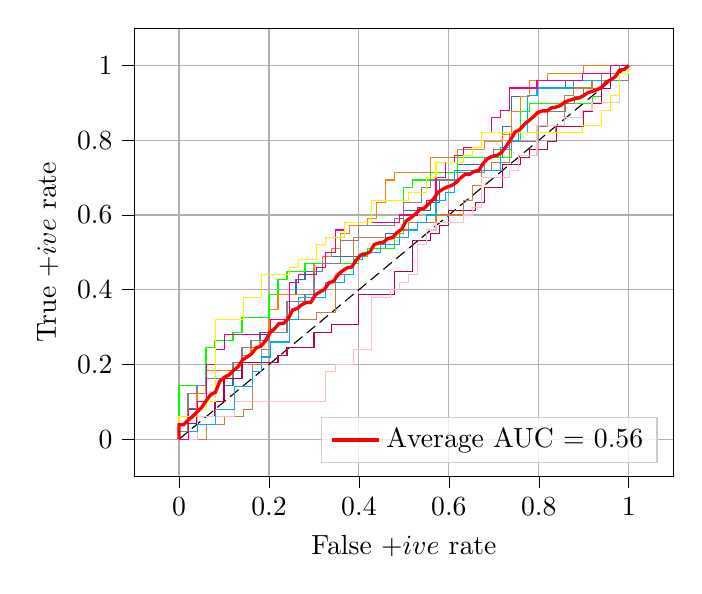
\begin{tikzpicture}
  \begin{axis}
    [
    ylabel={True $+ive$ rate},
    xlabel={False $+ive$ rate},
    tick align=outside,
    tick pos=left,
    ytick style={color=black},
    xtick style={color=black},
    grid style={gridgrey},
    xmajorgrids,
    ymajorgrids,
    legend cell align={left},
    legend columns=1,
    legend style={
      fill opacity=0.8,
      draw opacity=1,
      text opacity=1,
      at={(0.97,0.03)},
      anchor=south east,
      draw=legendgray,
    },
    ]

    \addplot[black, dashed, dash pattern=on 4pt off 2pt, forget plot] table {
      0 0
      1 1
    };


    \addplot[thin, color=steelblue, forget plot] table {
      0.0 0.0
      0.0 0.02040816326530612
      0.0 0.061224489795918366
      0.02 0.061224489795918366
      0.02 0.08163265306122448
      0.04 0.08163265306122448
      0.04 0.10204081632653061
      0.1 0.10204081632653061
      0.1 0.14285714285714285
      0.12 0.14285714285714285
      0.12 0.1836734693877551
      0.14 0.1836734693877551
      0.14 0.22448979591836735
      0.16 0.22448979591836735
      0.16 0.2653061224489796
      0.18 0.2653061224489796
      0.18 0.2857142857142857
      0.2 0.2857142857142857
      0.2 0.3469387755102041
      0.22 0.3469387755102041
      0.22 0.3877551020408163
      0.26 0.3877551020408163
      0.26 0.42857142857142855
      0.28 0.42857142857142855
      0.28 0.4489795918367347
      0.3 0.4489795918367347
      0.3 0.46938775510204084
      0.32 0.46938775510204084
      0.32 0.4897959183673469
      0.42 0.4897959183673469
      0.42 0.5102040816326531
      0.46 0.5102040816326531
      0.46 0.5510204081632653
      0.5 0.5510204081632653
      0.5 0.6122448979591837
      0.56 0.6122448979591837
      0.56 0.6326530612244898
      0.58 0.6326530612244898
      0.58 0.6938775510204082
      0.62 0.6938775510204082
      0.62 0.7346938775510204
      0.68 0.7346938775510204
      0.68 0.7551020408163265
      0.72 0.7551020408163265
      0.72 0.8367346938775511
      0.74 0.8367346938775511
      0.74 0.9183673469387755
      0.78 0.9183673469387755
      0.78 0.9387755102040817
      0.86 0.9387755102040817
      0.86 0.9591836734693877
      0.94 0.9591836734693877
      0.94 0.9795918367346939
      0.96 0.9795918367346939
      0.96 1.0
      1.0 1.0
    };


    \addplot[thin, color=darkorange, forget plot] table {
      0.0 0.0
      0.0 0.02040816326530612
      0.0 0.061224489795918366
      0.04 0.061224489795918366
      0.04 0.12244897959183673
      0.06 0.12244897959183673
      0.06 0.1836734693877551
      0.12 0.1836734693877551
      0.12 0.20408163265306123
      0.14 0.20408163265306123
      0.14 0.22448979591836735
      0.16 0.22448979591836735
      0.16 0.24489795918367346
      0.18 0.24489795918367346
      0.18 0.2653061224489796
      0.2 0.2653061224489796
      0.2 0.3469387755102041
      0.22 0.3469387755102041
      0.22 0.3877551020408163
      0.3 0.3877551020408163
      0.3 0.46938775510204084
      0.32 0.46938775510204084
      0.32 0.4897959183673469
      0.34 0.4897959183673469
      0.34 0.5102040816326531
      0.36 0.5102040816326531
      0.36 0.5510204081632653
      0.38 0.5510204081632653
      0.38 0.5714285714285714
      0.42 0.5714285714285714
      0.42 0.5918367346938775
      0.44 0.5918367346938775
      0.44 0.6326530612244898
      0.46 0.6326530612244898
      0.46 0.6938775510204082
      0.48 0.6938775510204082
      0.48 0.7142857142857143
      0.56 0.7142857142857143
      0.56 0.7551020408163265
      0.62 0.7551020408163265
      0.62 0.7755102040816326
      0.68 0.7755102040816326
      0.68 0.7959183673469388
      0.72 0.7959183673469388
      0.72 0.8163265306122449
      0.74 0.8163265306122449
      0.74 0.8775510204081632
      0.76 0.8775510204081632
      0.76 0.9183673469387755
      0.78 0.9183673469387755
      0.78 0.9591836734693877
      0.82 0.9591836734693877
      0.82 0.9795918367346939
      0.9 0.9795918367346939
      0.9 1.0
      1.0 1.0
    };


    \addplot[thin, color=green, forget plot] table {
      0.0 0.0
      0.0 0.02040816326530612
      0.0 0.14285714285714285
      0.06 0.14285714285714285
      0.06 0.24489795918367346
      0.08 0.24489795918367346
      0.08 0.2653061224489796
      0.12 0.2653061224489796
      0.12 0.2857142857142857
      0.14 0.2857142857142857
      0.14 0.32653061224489793
      0.2 0.32653061224489793
      0.2 0.3877551020408163
      0.22 0.3877551020408163
      0.22 0.42857142857142855
      0.24 0.42857142857142855
      0.24 0.4489795918367347
      0.28 0.4489795918367347
      0.28 0.46938775510204084
      0.4 0.46938775510204084
      0.4 0.4897959183673469
      0.42 0.4897959183673469
      0.42 0.5102040816326531
      0.48 0.5102040816326531
      0.48 0.5510204081632653
      0.5 0.5510204081632653
      0.5 0.673469387755102
      0.52 0.673469387755102
      0.52 0.6938775510204082
      0.56 0.6938775510204082
      0.56 0.7142857142857143
      0.62 0.7142857142857143
      0.62 0.7551020408163265
      0.74 0.7551020408163265
      0.74 0.7959183673469388
      0.76 0.7959183673469388
      0.76 0.8775510204081632
      0.78 0.8775510204081632
      0.78 0.8979591836734694
      0.92 0.8979591836734694
      0.92 0.9183673469387755
      0.94 0.9183673469387755
      0.94 0.9795918367346939
      0.98 0.9795918367346939
      0.98 1.0
      1.0 1.0
    };


    \addplot[thin, color=gray, forget plot] table {
      0.0 0.0
      0.0 0.02040816326530612
      0.02 0.02040816326530612
      0.02 0.12244897959183673
      0.04 0.12244897959183673
      0.04 0.14285714285714285
      0.06 0.14285714285714285
      0.06 0.16326530612244897
      0.12 0.16326530612244897
      0.12 0.20408163265306123
      0.14 0.20408163265306123
      0.14 0.24489795918367346
      0.16 0.24489795918367346
      0.16 0.2653061224489796
      0.2 0.2653061224489796
      0.2 0.2857142857142857
      0.24 0.2857142857142857
      0.24 0.3673469387755102
      0.28 0.3673469387755102
      0.28 0.3877551020408163
      0.3 0.3877551020408163
      0.3 0.4489795918367347
      0.32 0.4489795918367347
      0.32 0.46938775510204084
      0.36 0.46938775510204084
      0.36 0.5306122448979592
      0.4 0.5306122448979592
      0.4 0.5714285714285714
      0.48 0.5714285714285714
      0.48 0.5918367346938775
      0.5 0.5918367346938775
      0.5 0.6326530612244898
      0.54 0.6326530612244898
      0.54 0.673469387755102
      0.56 0.673469387755102
      0.56 0.6938775510204082
      0.62 0.6938775510204082
      0.62 0.7142857142857143
      0.68 0.7142857142857143
      0.68 0.7551020408163265
      0.7 0.7551020408163265
      0.7 0.7755102040816326
      0.74 0.7755102040816326
      0.74 0.7959183673469388
      0.8 0.7959183673469388
      0.8 0.8367346938775511
      0.82 0.8367346938775511
      0.82 0.8775510204081632
      0.86 0.8775510204081632
      0.86 0.8979591836734694
      0.88 0.8979591836734694
      0.88 0.9183673469387755
      0.9 0.9183673469387755
      0.9 0.9387755102040817
      0.94 0.9387755102040817
      0.94 0.9591836734693877
      1.0 0.9591836734693877
      1.0 1.0
    };


    \addplot[thin, color=purple, forget plot] table {
      0.0 0.0
      0.0 0.02040816326530612
      0.0 0.04081632653061224
      0.04 0.04081632653061224
      0.04 0.061224489795918366
      0.08 0.061224489795918366
      0.08 0.10204081632653061
      0.1 0.10204081632653061
      0.1 0.16326530612244897
      0.14 0.16326530612244897
      0.14 0.20408163265306123
      0.22 0.20408163265306123
      0.22 0.22448979591836735
      0.24 0.22448979591836735
      0.24 0.24489795918367346
      0.3 0.24489795918367346
      0.3 0.2857142857142857
      0.34 0.2857142857142857
      0.34 0.30612244897959184
      0.4 0.30612244897959184
      0.4 0.3877551020408163
      0.48 0.3877551020408163
      0.48 0.4489795918367347
      0.52 0.4489795918367347
      0.52 0.5306122448979592
      0.56 0.5306122448979592
      0.56 0.5510204081632653
      0.58 0.5510204081632653
      0.58 0.5714285714285714
      0.6 0.5714285714285714
      0.6 0.6122448979591837
      0.66 0.6122448979591837
      0.66 0.6326530612244898
      0.68 0.6326530612244898
      0.68 0.673469387755102
      0.72 0.673469387755102
      0.72 0.7346938775510204
      0.76 0.7346938775510204
      0.76 0.7551020408163265
      0.78 0.7551020408163265
      0.78 0.7755102040816326
      0.82 0.7755102040816326
      0.82 0.7959183673469388
      0.84 0.7959183673469388
      0.84 0.8367346938775511
      0.9 0.8367346938775511
      0.9 0.8775510204081632
      0.92 0.8775510204081632
      0.92 0.8979591836734694
      0.94 0.8979591836734694
      0.94 0.9387755102040817
      0.96 0.9387755102040817
      0.96 1.0
      1.0 1.0
    };


    \addplot[thin, color=brown, forget plot] table {
      0.0 0.0
      0.02040816326530612 0.0
      0.061224489795918366 0.0
      0.061224489795918366 0.04
      0.10204081632653061 0.04
      0.10204081632653061 0.06
      0.14285714285714285 0.06
      0.14285714285714285 0.08
      0.16326530612244897 0.08
      0.16326530612244897 0.2
      0.1836734693877551 0.2
      0.1836734693877551 0.24
      0.20408163265306123 0.24
      0.20408163265306123 0.26
      0.24489795918367346 0.26
      0.24489795918367346 0.32
      0.30612244897959184 0.32
      0.30612244897959184 0.34
      0.3469387755102041 0.34
      0.3469387755102041 0.44
      0.3877551020408163 0.44
      0.3877551020408163 0.54
      0.4897959183673469 0.54
      0.4897959183673469 0.56
      0.5102040816326531 0.56
      0.5102040816326531 0.58
      0.5714285714285714 0.58
      0.5714285714285714 0.6
      0.6326530612244898 0.6
      0.6326530612244898 0.64
      0.6530612244897959 0.64
      0.6530612244897959 0.68
      0.673469387755102 0.68
      0.673469387755102 0.72
      0.6938775510204082 0.72
      0.6938775510204082 0.74
      0.7346938775510204 0.74
      0.7346938775510204 0.82
      0.8367346938775511 0.82
      0.8367346938775511 0.84
      0.8571428571428571 0.84
      0.8571428571428571 0.92
      0.8775510204081632 0.92
      0.8775510204081632 0.94
      0.9183673469387755 0.94
      0.9183673469387755 0.96
      0.9387755102040817 0.96
      0.9387755102040817 0.98
      1.0 0.98
      1.0 1.0
    };


    \addplot[thin, color=pink, forget plot] table {
      0.0 0.0
      0.02040816326530612 0.0
      0.04081632653061224 0.0
      0.04081632653061224 0.06
      0.12244897959183673 0.06
      0.12244897959183673 0.1
      0.32653061224489793 0.1
      0.32653061224489793 0.18
      0.3469387755102041 0.18
      0.3469387755102041 0.2
      0.3877551020408163 0.2
      0.3877551020408163 0.24
      0.42857142857142855 0.24
      0.42857142857142855 0.38
      0.46938775510204084 0.38
      0.46938775510204084 0.4
      0.4897959183673469 0.4
      0.4897959183673469 0.42
      0.5102040816326531 0.42
      0.5102040816326531 0.44
      0.5306122448979592 0.44
      0.5306122448979592 0.52
      0.5510204081632653 0.52
      0.5510204081632653 0.56
      0.5714285714285714 0.56
      0.5714285714285714 0.58
      0.6326530612244898 0.58
      0.6326530612244898 0.6
      0.6530612244897959 0.6
      0.6530612244897959 0.62
      0.673469387755102 0.62
      0.673469387755102 0.7
      0.7346938775510204 0.7
      0.7346938775510204 0.72
      0.7551020408163265 0.72
      0.7551020408163265 0.76
      0.7959183673469388 0.76
      0.7959183673469388 0.84
      0.8571428571428571 0.84
      0.8571428571428571 0.86
      0.8979591836734694 0.86
      0.8979591836734694 0.88
      0.9183673469387755 0.88
      0.9183673469387755 0.9
      0.9795918367346939 0.9
      0.9795918367346939 0.98
      1.0 0.98
      1.0 1.0
    };


    \addplot[thin, color=cyan, forget plot] table {
      0.0 0.0
      0.02040816326530612 0.0
      0.02040816326530612 0.02
      0.04081632653061224 0.02
      0.04081632653061224 0.04
      0.08163265306122448 0.04
      0.08163265306122448 0.08
      0.12244897959183673 0.08
      0.12244897959183673 0.14
      0.16326530612244897 0.14
      0.16326530612244897 0.18
      0.1836734693877551 0.18
      0.1836734693877551 0.22
      0.20408163265306123 0.22
      0.20408163265306123 0.26
      0.24489795918367346 0.26
      0.24489795918367346 0.32
      0.2653061224489796 0.32
      0.2653061224489796 0.38
      0.32653061224489793 0.38
      0.32653061224489793 0.42
      0.3673469387755102 0.42
      0.3673469387755102 0.44
      0.3877551020408163 0.44
      0.3877551020408163 0.48
      0.40816326530612246 0.48
      0.40816326530612246 0.5
      0.4489795918367347 0.5
      0.4489795918367347 0.52
      0.4897959183673469 0.52
      0.4897959183673469 0.54
      0.5102040816326531 0.54
      0.5102040816326531 0.56
      0.5306122448979592 0.56
      0.5306122448979592 0.58
      0.5510204081632653 0.58
      0.5510204081632653 0.6
      0.5714285714285714 0.6
      0.5714285714285714 0.64
      0.5918367346938775 0.64
      0.5918367346938775 0.66
      0.6122448979591837 0.66
      0.6122448979591837 0.72
      0.7142857142857143 0.72
      0.7142857142857143 0.78
      0.7346938775510204 0.78
      0.7346938775510204 0.8
      0.7551020408163265 0.8
      0.7551020408163265 0.82
      0.7755102040816326 0.82
      0.7755102040816326 0.92
      0.7959183673469388 0.92
      0.7959183673469388 0.94
      0.8775510204081632 0.94
      0.8775510204081632 0.96
      0.9795918367346939 0.96
      0.9795918367346939 1.0
      1.0 1.0
    };


    \addplot[thin, color=magenta, forget plot] table {
      0.0 0.0
      0.02040816326530612 0.0
      0.02040816326530612 0.08
      0.04081632653061224 0.08
      0.04081632653061224 0.1
      0.061224489795918366 0.1
      0.061224489795918366 0.2
      0.08163265306122448 0.2
      0.08163265306122448 0.24
      0.10204081632653061 0.24
      0.10204081632653061 0.28
      0.20408163265306123 0.28
      0.20408163265306123 0.32
      0.24489795918367346 0.32
      0.24489795918367346 0.42
      0.2653061224489796 0.42
      0.2653061224489796 0.44
      0.30612244897959184 0.44
      0.30612244897959184 0.46
      0.32653061224489793 0.46
      0.32653061224489793 0.5
      0.3469387755102041 0.5
      0.3469387755102041 0.56
      0.3673469387755102 0.56
      0.3673469387755102 0.58
      0.4897959183673469 0.58
      0.4897959183673469 0.6
      0.5306122448979592 0.6
      0.5306122448979592 0.62
      0.5510204081632653 0.62
      0.5510204081632653 0.64
      0.5714285714285714 0.64
      0.5714285714285714 0.7
      0.5918367346938775 0.7
      0.5918367346938775 0.74
      0.6122448979591837 0.74
      0.6122448979591837 0.76
      0.6326530612244898 0.76
      0.6326530612244898 0.78
      0.673469387755102 0.78
      0.673469387755102 0.82
      0.6938775510204082 0.82
      0.6938775510204082 0.86
      0.7142857142857143 0.86
      0.7142857142857143 0.88
      0.7346938775510204 0.88
      0.7346938775510204 0.94
      0.7959183673469388 0.94
      0.7959183673469388 0.96
      0.8979591836734694 0.96
      0.8979591836734694 0.98
      0.9591836734693877 0.98
      0.9591836734693877 1.0
      1.0 1.0
    };


    \addplot[thin, color=yellow, forget plot] table {
      0.0 0.0
      0.0 0.02
      0.0 0.06
      0.04081632653061224 0.06
      0.04081632653061224 0.08
      0.061224489795918366 0.08
      0.061224489795918366 0.1
      0.08163265306122448 0.1
      0.08163265306122448 0.32
      0.14285714285714285 0.32
      0.14285714285714285 0.38
      0.1836734693877551 0.38
      0.1836734693877551 0.44
      0.24489795918367346 0.44
      0.24489795918367346 0.46
      0.2653061224489796 0.46
      0.2653061224489796 0.48
      0.30612244897959184 0.48
      0.30612244897959184 0.52
      0.32653061224489793 0.52
      0.32653061224489793 0.54
      0.3673469387755102 0.54
      0.3673469387755102 0.58
      0.42857142857142855 0.58
      0.42857142857142855 0.64
      0.5102040816326531 0.64
      0.5102040816326531 0.66
      0.5510204081632653 0.66
      0.5510204081632653 0.7
      0.5714285714285714 0.7
      0.5714285714285714 0.74
      0.6326530612244898 0.74
      0.6326530612244898 0.76
      0.6530612244897959 0.76
      0.6530612244897959 0.78
      0.673469387755102 0.78
      0.673469387755102 0.82
      0.8979591836734694 0.82
      0.8979591836734694 0.84
      0.9387755102040817 0.84
      0.9387755102040817 0.88
      0.9591836734693877 0.88
      0.9591836734693877 0.92
      0.9795918367346939 0.92
      0.9795918367346939 0.98
      1.0 0.98
      1.0 1.0
    };

    \addlegendentry{Average AUC = $0.56$}
    \addplot[very thick, red] table {
      0 0
      0.0 0.03865306122448979
      0.010101010101010102 0.03865306122448979
      0.020202020202020204 0.05089795918367347
      0.030303030303030304 0.06089795918367347
      0.04040404040404041 0.07314285714285713
      0.05050505050505051 0.08514285714285712
      0.06060606060606061 0.10351020408163263
      0.07070707070707072 0.11951020408163264
      0.08080808080808081 0.12563265306122448
      0.09090909090909091 0.15563265306122448
      0.10101010101010102 0.16583673469387755
      0.11111111111111112 0.17183673469387756
      0.12121212121212122 0.18408163265306127
      0.13131313131313133 0.19408163265306128
      0.14141414141414144 0.21244897959183678
      0.15151515151515152 0.2204489795918368
      0.16161616161616163 0.22861224489795923
      0.17171717171717174 0.2446122448979592
      0.18181818181818182 0.2486938775510204
      0.19191919191919193 0.2626938775510204
      0.20202020202020204 0.2851428571428572
      0.21212121212121213 0.2951428571428571
      0.22222222222222224 0.30942857142857144
      0.23232323232323235 0.30942857142857144
      0.24242424242424243 0.3216734693877551
      0.25252525252525254 0.3456734693877551
      0.26262626262626265 0.34975510204081633
      0.27272727272727276 0.35975510204081634
      0.2828282828282829 0.36587755102040814
      0.29292929292929293 0.36587755102040814
      0.30303030303030304 0.38628571428571423
      0.31313131313131315 0.39428571428571424
      0.32323232323232326 0.40040816326530615
      0.33333333333333337 0.41840816326530617
      0.3434343434343435 0.42248979591836733
      0.3535353535353536 0.4404897959183674
      0.36363636363636365 0.4506938775510204
      0.37373737373737376 0.4586938775510204
      0.38383838383838387 0.46073469387755106
      0.393939393939394 0.478734693877551
      0.4040404040404041 0.49302040816326526
      0.4141414141414142 0.4950204081632653
      0.42424242424242425 0.5011428571428571
      0.43434343434343436 0.5211428571428571
      0.4444444444444445 0.5252244897959183
      0.4545454545454546 0.5272244897959182
      0.4646464646464647 0.5374285714285713
      0.4747474747474748 0.5394285714285714
      0.48484848484848486 0.5537142857142856
      0.494949494949495 0.5617142857142856
      0.5050505050505051 0.5841632653061224
      0.5151515151515152 0.5921632653061225
      0.5252525252525253 0.6023673469387756
      0.5353535353535354 0.6143673469387756
      0.5454545454545455 0.6184489795918368
      0.5555555555555556 0.6304489795918367
      0.5656565656565657 0.6426938775510204
      0.5757575757575758 0.6606938775510204
      0.5858585858585859 0.6688571428571428
      0.595959595959596 0.6748571428571429
      0.6060606060606061 0.6789387755102041
      0.6161616161616162 0.686938775510204
      0.6262626262626263 0.6991836734693877
      0.6363636363636365 0.7091836734693877
      0.6464646464646465 0.7091836734693877
      0.6565656565656566 0.7171836734693878
      0.6666666666666667 0.7192244897959184
      0.6767676767676768 0.7392244897959184
      0.686868686868687 0.7514693877551021
      0.696969696969697 0.757469387755102
      0.7070707070707072 0.7595102040816327
      0.7171717171717172 0.7675102040816327
      0.7272727272727273 0.7838367346938776
      0.7373737373737375 0.8018367346938776
      0.7474747474747475 0.8222448979591837
      0.7575757575757577 0.8282448979591838
      0.7676767676767677 0.842530612244898
      0.7777777777777778 0.8525306122448979
      0.787878787878788 0.862734693877551
      0.797979797979798 0.8747346938775509
      0.8080808080808082 0.8788163265306121
      0.8181818181818182 0.8788163265306121
      0.8282828282828284 0.8869795918367348
      0.8383838383838385 0.8889795918367348
      0.8484848484848485 0.8930612244897957
      0.8585858585858587 0.903061224489796
      0.8686868686868687 0.9071428571428573
      0.8787878787878789 0.9111428571428573
      0.888888888888889 0.9131836734693877
      0.8989898989898991 0.9191836734693878
      0.9090909090909092 0.9273469387755103
      0.9191919191919192 0.9313469387755102
      0.9292929292929294 0.9354285714285714
      0.9393939393939394 0.9414285714285715
      0.9494949494949496 0.9557142857142857
      0.9595959595959597 0.9617142857142857
      0.9696969696969697 0.9698775510204081
      0.9797979797979799 0.9878775510204083
      0.98989898989899 0.9899183673469389
      1.0 1.0
    };
  \end{axis}
\end{tikzpicture}}
              \captionsetup{justification=centering}
              \caption{Without data leak}
            \end{subfigure}
            \caption{XGBoost results on \textbf{H\_990} dataset}\label{fig:xgb_h990}
        \end{figure}

        \begin{figure}[H]
            \centering
            \begin{subfigure}{0.45\textwidth}
              \centering
              \resizebox{\textwidth}{!}{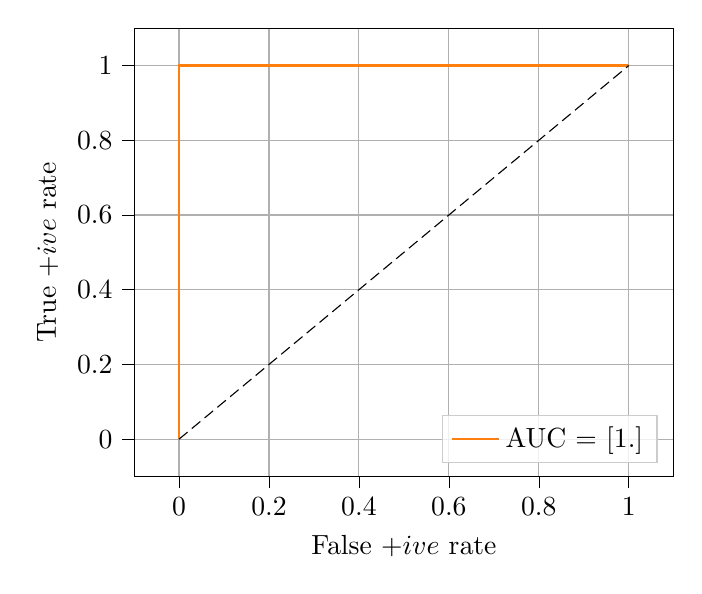
\begin{tikzpicture}
  \begin{axis}
    [
    ylabel={True $+ive$ rate},
    xlabel={False $+ive$ rate},
    tick align=outside,
    tick pos=left,
    ytick style={color=black},
    xtick style={color=black},
    grid style={gridgrey},
    xmajorgrids,
    ymajorgrids,
    legend cell align={left},
    legend columns=1,
    legend style={
      fill opacity=0.8,
      draw opacity=1,
      text opacity=1,
      at={(0.97,0.03)},
      anchor=south east,
      draw=legendgray,
    },
    ]
    \addlegendentry{AUC = $[1.]$}
    \addplot[thick, darkorange] table {
      0.0 0.0
      0.0 0.01
      0.0 0.1
      0.0 0.12
      0.0 0.2
      0.0 0.26
      0.0 0.3
      0.0 0.33
      0.0 0.62
      0.0 0.64
      0.0 0.66
      0.0 0.69
      0.0 0.77
      0.0 0.8
      0.0 0.82
      0.0 0.84
      0.0 0.87
      0.0 0.89
      0.0 1.0
      1.0 1.0
    };
    \addplot[black, dashed, dash pattern=on 4pt off 2pt] table {
      0 0
      1 1
    };
  \end{axis}
\end{tikzpicture}
}
              \captionsetup{justification=centering}
              \caption{With data leak}
            \end{subfigure}%
            \hspace{0.05\textwidth}
            \begin{subfigure}{0.45\textwidth}
              \centering
              \resizebox{\textwidth}{!}{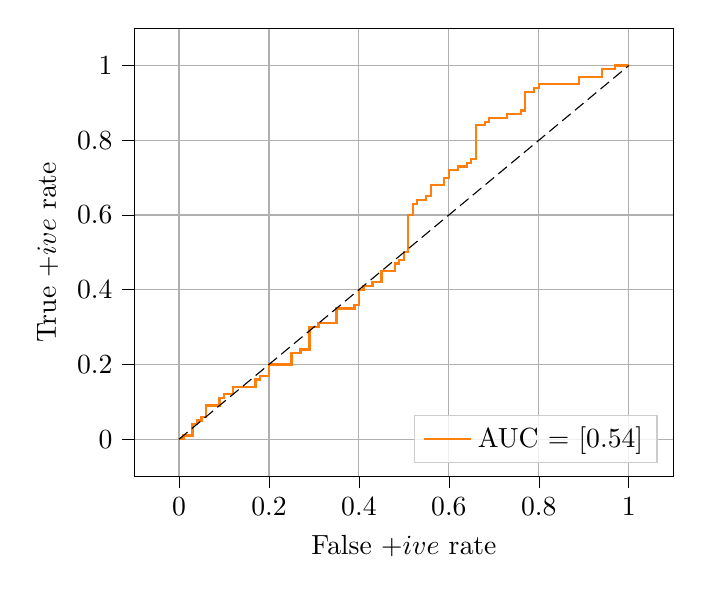
\begin{tikzpicture}
  \begin{axis}
    [
    ylabel={True $+ive$ rate},
    xlabel={False $+ive$ rate},
    tick align=outside,
    tick pos=left,
    ytick style={color=black},
    xtick style={color=black},
    grid style={gridgrey},
    xmajorgrids,
    ymajorgrids,
    legend cell align={left},
    legend columns=1,
    legend style={
      fill opacity=0.8,
      draw opacity=1,
      text opacity=1,
      at={(0.97,0.03)},
      anchor=south east,
      draw=legendgray,
    },
    ]
    \addlegendentry{AUC = $[0.54]$}
    \addplot[thick, darkorange] table {
      0.0 0.0
      0.01 0.0
      0.01 0.01
      0.03 0.01
      0.03 0.04
      0.04 0.04
      0.04 0.05
      0.05 0.05
      0.05 0.06
      0.06 0.06
      0.06 0.08
      0.06 0.09
      0.09 0.09
      0.09 0.11
      0.1 0.11
      0.1 0.12
      0.12 0.12
      0.12 0.14
      0.17 0.14
      0.17 0.16
      0.18 0.16
      0.18 0.17
      0.2 0.17
      0.2 0.2
      0.25 0.2
      0.25 0.23
      0.27 0.23
      0.27 0.24
      0.29 0.24
      0.29 0.3
      0.31 0.3
      0.31 0.31
      0.35 0.31
      0.35 0.35
      0.39 0.35
      0.39 0.36
      0.4 0.36
      0.4 0.4
      0.41 0.4
      0.41 0.41
      0.43 0.41
      0.43 0.42
      0.45 0.42
      0.45 0.45
      0.48 0.45
      0.48 0.47
      0.49 0.47
      0.49 0.48
      0.5 0.48
      0.5 0.5
      0.51 0.5
      0.51 0.51
      0.51 0.57
      0.51 0.6
      0.52 0.6
      0.52 0.63
      0.53 0.63
      0.53 0.64
      0.55 0.64
      0.55 0.65
      0.56 0.65
      0.56 0.68
      0.59 0.68
      0.59 0.7
      0.6 0.7
      0.6 0.72
      0.62 0.72
      0.62 0.73
      0.64 0.73
      0.64 0.74
      0.65 0.74
      0.65 0.75
      0.66 0.75
      0.66 0.79
      0.66 0.81
      0.66 0.84
      0.68 0.84
      0.68 0.85
      0.69 0.85
      0.69 0.86
      0.73 0.86
      0.73 0.87
      0.76 0.87
      0.76 0.88
      0.77 0.88
      0.77 0.91
      0.77 0.93
      0.79 0.93
      0.79 0.94
      0.8 0.94
      0.8 0.95
      0.89 0.95
      0.89 0.97
      0.94 0.97
      0.94 0.99
      0.97 0.99
      0.97 1.0
      1.0 1.0
    };
    \addplot[black, dashed, dash pattern=on 4pt off 2pt] table {
      0 0
      1 1
    };
  \end{axis}
\end{tikzpicture}}
              \captionsetup{justification=centering}
              \caption{Without data leak}
            \end{subfigure}
            \caption{XGBoost results on \textbf{H\_200} dataset}\label{fig:xgb_h200}
        \end{figure}

      \paragraph{Saccharomyces cerevisiae}
        \noindent
        \begin{table}[H]
            \centering
            \begin{minipage}{0.45\textwidth}
              \centering
              \begin{tabular}{lcc}
                \toprule
                \textbf{Metric} & \textbf{Data Leak} & \textbf{Fixed} \\
                \midrule
                Accuracy        & 95\%               & 59\%           \\
                MCC             & 0.89               & 0.18           \\
                Sensitivity     & 95\%               & 55\%           \\
                Specificity     & 95\%               & 63\%           \\
                \bottomrule
              \end{tabular}
              \caption{Results for S\_628 dataset}
            \end{minipage}%
            \hfill
            \begin{minipage}{0.45\textwidth}
              \centering
              \begin{tabular}{lcc}
                \toprule
                \textbf{Metric} & \textbf{Data Leak} & \textbf{Fixed} \\
                \midrule
                Accuracy        & 95\%               & 58\%           \\
                MCC             & 0.91               & 0.17           \\
                Sensitivity     & 97\%               & 50\%           \\
                Specificity     & 94\%               & 67\%           \\
                \bottomrule
              \end{tabular}
              \caption{Results for S\_200 dataset}
            \end{minipage}\label{tab:xgb_pstnpss_sc}
        \end{table}

        \begin{figure}[H]
            \centering
            \begin{subfigure}{0.47\textwidth}
              \centering
              \resizebox{\textwidth}{!}{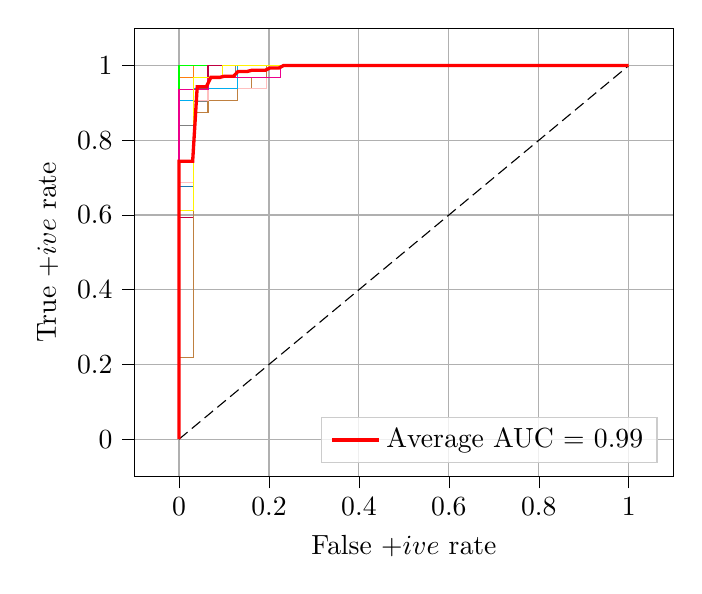
\begin{tikzpicture}
  \begin{axis}
    [
    ylabel={True $+ive$ rate},
    xlabel={False $+ive$ rate},
    tick align=outside,
    tick pos=left,
    ytick style={color=black},
    xtick style={color=black},
    grid style={gridgrey},
    xmajorgrids,
    ymajorgrids,
    legend cell align={left},
    legend columns=1,
    legend style={
      fill opacity=0.8,
      draw opacity=1,
      text opacity=1,
      at={(0.97,0.03)},
      anchor=south east,
      draw=legendgray,
    },
    ]

    \addplot[black, dashed, dash pattern=on 4pt off 2pt, forget plot] table {
      0 0
      1 1
    };


    \addplot[thin, color=steelblue, forget plot] table {
      0.0 0.0
      0.0 0.03225806451612903
      0.0 0.6774193548387096
      0.03125 0.6774193548387096
      0.03125 0.967741935483871
      0.0625 0.967741935483871
      0.0625 1.0
      1.0 1.0
    };


    \addplot[thin, color=darkorange, forget plot] table {
      0.0 0.0
      0.0 0.03225806451612903
      0.0 0.967741935483871
      0.03125 0.967741935483871
      0.03125 1.0
      1.0 1.0
    };


    \addplot[thin, color=green, forget plot] table {
      0.0 0.0
      0.0 0.03225806451612903
      0.0 1.0
      1.0 1.0
    };


    \addplot[thin, color=gray, forget plot] table {
      0.0 0.0
      0.0 0.03225806451612903
      0.0 0.8387096774193549
      0.03125 0.8387096774193549
      0.03125 0.9032258064516129
      0.0625 0.9032258064516129
      0.0625 0.967741935483871
      0.125 0.967741935483871
      0.125 1.0
      1.0 1.0
    };


    \addplot[thin, color=purple, forget plot] table {
      0.0 0.0
      0.0 0.03125
      0.0 0.59375
      0.03225806451612903 0.59375
      0.03225806451612903 0.9375
      0.06451612903225806 0.9375
      0.06451612903225806 1.0
      1.0 1.0
    };


    \addplot[thin, color=brown, forget plot] table {
      0.0 0.0
      0.0 0.03125
      0.0 0.21875
      0.03225806451612903 0.21875
      0.03225806451612903 0.875
      0.06451612903225806 0.875
      0.06451612903225806 0.90625
      0.12903225806451613 0.90625
      0.12903225806451613 0.9375
      0.16129032258064516 0.9375
      0.16129032258064516 0.96875
      0.1935483870967742 0.96875
      0.1935483870967742 1.0
      1.0 1.0
    };


    \addplot[thin, color=pink, forget plot] table {
      0.0 0.0
      0.0 0.03125
      0.0 0.6875
      0.03225806451612903 0.6875
      0.03225806451612903 0.90625
      0.06451612903225806 0.90625
      0.06451612903225806 0.9375
      0.1935483870967742 0.9375
      0.1935483870967742 0.96875
      0.22580645161290322 0.96875
      0.22580645161290322 1.0
      1.0 1.0
    };


    \addplot[thin, color=cyan, forget plot] table {
      0.0 0.0
      0.0 0.03125
      0.0 0.90625
      0.03225806451612903 0.90625
      0.03225806451612903 0.9375
      0.12903225806451613 0.9375
      0.12903225806451613 1.0
      1.0 1.0
    };


    \addplot[thin, color=magenta, forget plot] table {
      0.0 0.0
      0.0 0.03225806451612903
      0.0 0.9354838709677419
      0.06451612903225806 0.9354838709677419
      0.06451612903225806 0.967741935483871
      0.22580645161290322 0.967741935483871
      0.22580645161290322 1.0
      1.0 1.0
    };


    \addplot[thin, color=yellow, forget plot] table {
      0.0 0.0
      0.0 0.03225806451612903
      0.0 0.6129032258064516
      0.03225806451612903 0.6129032258064516
      0.03225806451612903 0.967741935483871
      0.0967741935483871 0.967741935483871
      0.0967741935483871 1.0
      1.0 1.0
    };

    \addlegendentry{Average AUC = $0.99$}
    \addplot[very thick, red] table {
      0 0
      0.0 0.743850806451613
      0.010101010101010102 0.743850806451613
      0.020202020202020204 0.743850806451613
      0.030303030303030304 0.743850806451613
      0.04040404040404041 0.9430443548387096
      0.05050505050505051 0.9430443548387096
      0.06060606060606061 0.9430443548387096
      0.07070707070707072 0.9684475806451612
      0.08080808080808081 0.9684475806451612
      0.09090909090909091 0.9684475806451612
      0.10101010101010102 0.9716733870967742
      0.11111111111111112 0.9716733870967742
      0.12121212121212122 0.9716733870967742
      0.13131313131313133 0.9842741935483872
      0.14141414141414144 0.9842741935483872
      0.15151515151515152 0.9842741935483872
      0.16161616161616163 0.9873991935483872
      0.17171717171717174 0.9873991935483872
      0.18181818181818182 0.9873991935483872
      0.19191919191919193 0.9873991935483872
      0.20202020202020204 0.9936491935483872
      0.21212121212121213 0.9936491935483872
      0.22222222222222224 0.9936491935483872
      0.23232323232323235 1.0
      0.24242424242424243 1.0
      0.25252525252525254 1.0
      0.26262626262626265 1.0
      0.27272727272727276 1.0
      0.2828282828282829 1.0
      0.29292929292929293 1.0
      0.30303030303030304 1.0
      0.31313131313131315 1.0
      0.32323232323232326 1.0
      0.33333333333333337 1.0
      0.3434343434343435 1.0
      0.3535353535353536 1.0
      0.36363636363636365 1.0
      0.37373737373737376 1.0
      0.38383838383838387 1.0
      0.393939393939394 1.0
      0.4040404040404041 1.0
      0.4141414141414142 1.0
      0.42424242424242425 1.0
      0.43434343434343436 1.0
      0.4444444444444445 1.0
      0.4545454545454546 1.0
      0.4646464646464647 1.0
      0.4747474747474748 1.0
      0.48484848484848486 1.0
      0.494949494949495 1.0
      0.5050505050505051 1.0
      0.5151515151515152 1.0
      0.5252525252525253 1.0
      0.5353535353535354 1.0
      0.5454545454545455 1.0
      0.5555555555555556 1.0
      0.5656565656565657 1.0
      0.5757575757575758 1.0
      0.5858585858585859 1.0
      0.595959595959596 1.0
      0.6060606060606061 1.0
      0.6161616161616162 1.0
      0.6262626262626263 1.0
      0.6363636363636365 1.0
      0.6464646464646465 1.0
      0.6565656565656566 1.0
      0.6666666666666667 1.0
      0.6767676767676768 1.0
      0.686868686868687 1.0
      0.696969696969697 1.0
      0.7070707070707072 1.0
      0.7171717171717172 1.0
      0.7272727272727273 1.0
      0.7373737373737375 1.0
      0.7474747474747475 1.0
      0.7575757575757577 1.0
      0.7676767676767677 1.0
      0.7777777777777778 1.0
      0.787878787878788 1.0
      0.797979797979798 1.0
      0.8080808080808082 1.0
      0.8181818181818182 1.0
      0.8282828282828284 1.0
      0.8383838383838385 1.0
      0.8484848484848485 1.0
      0.8585858585858587 1.0
      0.8686868686868687 1.0
      0.8787878787878789 1.0
      0.888888888888889 1.0
      0.8989898989898991 1.0
      0.9090909090909092 1.0
      0.9191919191919192 1.0
      0.9292929292929294 1.0
      0.9393939393939394 1.0
      0.9494949494949496 1.0
      0.9595959595959597 1.0
      0.9696969696969697 1.0
      0.9797979797979799 1.0
      0.98989898989899 1.0
      1.0 1.0
    };
  \end{axis}
\end{tikzpicture}
}
              \captionsetup{justification=centering}
              \caption{With data leak}
            \end{subfigure}%
            \hspace{0.05\textwidth}
            \begin{subfigure}{0.47\textwidth}
              \centering
              \resizebox{\textwidth}{!}{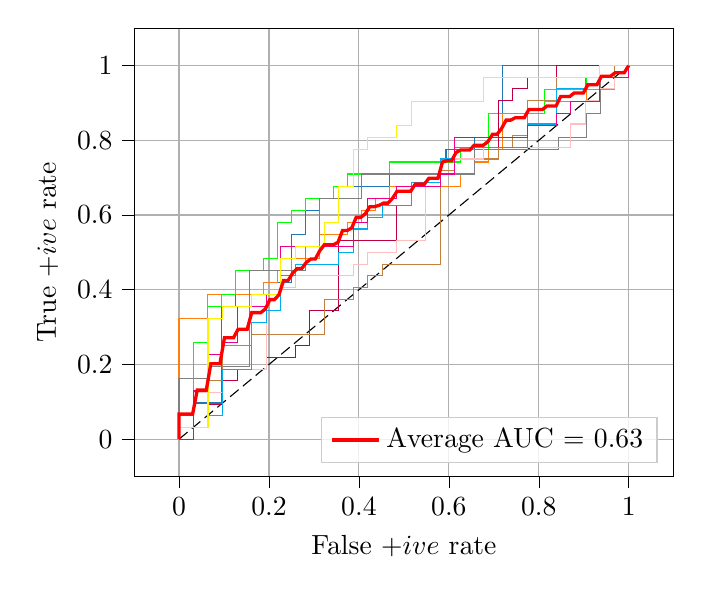
\begin{tikzpicture}
  \begin{axis}
    [
    ylabel={True $+ive$ rate},
    xlabel={False $+ive$ rate},
    tick align=outside,
    tick pos=left,
    ytick style={color=black},
    xtick style={color=black},
    grid style={gridgrey},
    xmajorgrids,
    ymajorgrids,
    legend cell align={left},
    legend columns=1,
    legend style={
      fill opacity=0.8,
      draw opacity=1,
      text opacity=1,
      at={(0.97,0.03)},
      anchor=south east,
      draw=legendgray,
    },
    ]

    \addplot[black, dashed, dash pattern=on 4pt off 2pt, forget plot] table {
      0 0
      1 1
    };


    \addplot[thin, color=steelblue, forget plot] table {
      0.0 0.0
      0.0 0.03225806451612903
      0.0 0.06451612903225806
      0.03125 0.06451612903225806
      0.03125 0.0967741935483871
      0.09375 0.0967741935483871
      0.09375 0.3548387096774194
      0.125 0.3548387096774194
      0.125 0.3870967741935484
      0.1875 0.3870967741935484
      0.1875 0.41935483870967744
      0.25 0.41935483870967744
      0.25 0.5483870967741935
      0.28125 0.5483870967741935
      0.28125 0.6129032258064516
      0.3125 0.6129032258064516
      0.3125 0.6451612903225806
      0.34375 0.6451612903225806
      0.34375 0.6774193548387096
      0.46875 0.6774193548387096
      0.46875 0.7419354838709677
      0.59375 0.7419354838709677
      0.59375 0.7741935483870968
      0.65625 0.7741935483870968
      0.65625 0.8064516129032258
      0.6875 0.8064516129032258
      0.6875 0.8709677419354839
      0.71875 0.8709677419354839
      0.71875 1.0
      1.0 1.0
    };


    \addplot[thin, color=darkorange, forget plot] table {
      0.0 0.0
      0.0 0.03225806451612903
      0.0 0.3225806451612903
      0.0625 0.3225806451612903
      0.0625 0.3870967741935484
      0.1875 0.3870967741935484
      0.1875 0.41935483870967744
      0.21875 0.41935483870967744
      0.21875 0.45161290322580644
      0.25 0.45161290322580644
      0.25 0.4838709677419355
      0.3125 0.4838709677419355
      0.3125 0.5483870967741935
      0.375 0.5483870967741935
      0.375 0.5806451612903226
      0.40625 0.5806451612903226
      0.40625 0.6129032258064516
      0.4375 0.6129032258064516
      0.4375 0.6451612903225806
      0.46875 0.6451612903225806
      0.46875 0.6774193548387096
      0.625 0.6774193548387096
      0.625 0.7096774193548387
      0.65625 0.7096774193548387
      0.65625 0.7419354838709677
      0.6875 0.7419354838709677
      0.6875 0.7741935483870968
      0.71875 0.7741935483870968
      0.71875 0.8709677419354839
      0.8125 0.8709677419354839
      0.8125 0.9032258064516129
      0.90625 0.9032258064516129
      0.90625 0.9354838709677419
      0.96875 0.9354838709677419
      0.96875 0.967741935483871
      1.0 0.967741935483871
      1.0 1.0
    };


    \addplot[thin, color=green, forget plot] table {
      0.0 0.0
      0.0 0.03225806451612903
      0.03125 0.03225806451612903
      0.03125 0.25806451612903225
      0.0625 0.25806451612903225
      0.0625 0.3548387096774194
      0.09375 0.3548387096774194
      0.09375 0.3870967741935484
      0.125 0.3870967741935484
      0.125 0.45161290322580644
      0.1875 0.45161290322580644
      0.1875 0.4838709677419355
      0.21875 0.4838709677419355
      0.21875 0.5806451612903226
      0.25 0.5806451612903226
      0.25 0.6129032258064516
      0.28125 0.6129032258064516
      0.28125 0.6451612903225806
      0.34375 0.6451612903225806
      0.34375 0.6774193548387096
      0.375 0.6774193548387096
      0.375 0.7096774193548387
      0.46875 0.7096774193548387
      0.46875 0.7419354838709677
      0.625 0.7419354838709677
      0.625 0.7741935483870968
      0.6875 0.7741935483870968
      0.6875 0.8709677419354839
      0.8125 0.8709677419354839
      0.8125 0.9354838709677419
      0.90625 0.9354838709677419
      0.90625 0.967741935483871
      1.0 0.967741935483871
      1.0 1.0
    };


    \addplot[thin, color=gray, forget plot] table {
      0.0 0.0
      0.0 0.03225806451612903
      0.0 0.16129032258064516
      0.0625 0.16129032258064516
      0.0625 0.1935483870967742
      0.15625 0.1935483870967742
      0.15625 0.45161290322580644
      0.28125 0.45161290322580644
      0.28125 0.5161290322580645
      0.3125 0.5161290322580645
      0.3125 0.6451612903225806
      0.40625 0.6451612903225806
      0.40625 0.7096774193548387
      0.65625 0.7096774193548387
      0.65625 0.7741935483870968
      0.84375 0.7741935483870968
      0.84375 0.8064516129032258
      0.90625 0.8064516129032258
      0.90625 0.8709677419354839
      0.9375 0.8709677419354839
      0.9375 0.967741935483871
      1.0 0.967741935483871
      1.0 1.0
    };


    \addplot[thin, color=purple, forget plot] table {
      0.0 0.0
      0.03225806451612903 0.0
      0.03225806451612903 0.03125
      0.06451612903225806 0.03125
      0.06451612903225806 0.09375
      0.0967741935483871 0.09375
      0.0967741935483871 0.15625
      0.12903225806451613 0.15625
      0.12903225806451613 0.1875
      0.1935483870967742 0.1875
      0.1935483870967742 0.21875
      0.25806451612903225 0.21875
      0.25806451612903225 0.25
      0.2903225806451613 0.25
      0.2903225806451613 0.34375
      0.3548387096774194 0.34375
      0.3548387096774194 0.53125
      0.4838709677419355 0.53125
      0.4838709677419355 0.625
      0.5161290322580645 0.625
      0.5161290322580645 0.6875
      0.5806451612903226 0.6875
      0.5806451612903226 0.71875
      0.6129032258064516 0.71875
      0.6129032258064516 0.78125
      0.7096774193548387 0.78125
      0.7096774193548387 0.90625
      0.7419354838709677 0.90625
      0.7419354838709677 0.9375
      0.7741935483870968 0.9375
      0.7741935483870968 0.96875
      0.8387096774193549 0.96875
      0.8387096774193549 1.0
      1.0 1.0
    };


    \addplot[thin, color=brown, forget plot] table {
      0.0 0.0
      0.03225806451612903 0.0
      0.03225806451612903 0.125
      0.06451612903225806 0.125
      0.06451612903225806 0.15625
      0.0967741935483871 0.15625
      0.0967741935483871 0.25
      0.16129032258064516 0.25
      0.16129032258064516 0.28125
      0.3225806451612903 0.28125
      0.3225806451612903 0.375
      0.3870967741935484 0.375
      0.3870967741935484 0.40625
      0.41935483870967744 0.40625
      0.41935483870967744 0.4375
      0.45161290322580644 0.4375
      0.45161290322580644 0.46875
      0.5806451612903226 0.46875
      0.5806451612903226 0.71875
      0.6129032258064516 0.71875
      0.6129032258064516 0.75
      0.7096774193548387 0.75
      0.7096774193548387 0.78125
      0.7419354838709677 0.78125
      0.7419354838709677 0.8125
      0.7741935483870968 0.8125
      0.7741935483870968 0.90625
      0.8387096774193549 0.90625
      0.8387096774193549 0.96875
      0.967741935483871 0.96875
      0.967741935483871 1.0
      1.0 1.0
    };


    \addplot[thin, color=pink, forget plot] table {
      0.0 0.0
      0.0 0.03125
      0.03225806451612903 0.03125
      0.03225806451612903 0.125
      0.0967741935483871 0.125
      0.0967741935483871 0.1875
      0.1935483870967742 0.1875
      0.1935483870967742 0.34375
      0.22580645161290322 0.34375
      0.22580645161290322 0.40625
      0.25806451612903225 0.40625
      0.25806451612903225 0.4375
      0.3870967741935484 0.4375
      0.3870967741935484 0.46875
      0.41935483870967744 0.46875
      0.41935483870967744 0.5
      0.4838709677419355 0.5
      0.4838709677419355 0.53125
      0.5483870967741935 0.53125
      0.5483870967741935 0.6875
      0.5806451612903226 0.6875
      0.5806451612903226 0.75
      0.6774193548387096 0.75
      0.6774193548387096 0.78125
      0.8709677419354839 0.78125
      0.8709677419354839 0.84375
      0.9032258064516129 0.84375
      0.9032258064516129 0.90625
      0.9354838709677419 0.90625
      0.9354838709677419 0.9375
      0.967741935483871 0.9375
      0.967741935483871 0.96875
      1.0 0.96875
      1.0 1.0
    };


    \addplot[thin, color=cyan, forget plot] table {
      0.0 0.0
      0.0 0.03125
      0.06451612903225806 0.03125
      0.06451612903225806 0.0625
      0.0967741935483871 0.0625
      0.0967741935483871 0.1875
      0.16129032258064516 0.1875
      0.16129032258064516 0.3125
      0.1935483870967742 0.3125
      0.1935483870967742 0.34375
      0.22580645161290322 0.34375
      0.22580645161290322 0.4375
      0.25806451612903225 0.4375
      0.25806451612903225 0.46875
      0.3548387096774194 0.46875
      0.3548387096774194 0.5
      0.3870967741935484 0.5
      0.3870967741935484 0.5625
      0.41935483870967744 0.5625
      0.41935483870967744 0.59375
      0.45161290322580644 0.59375
      0.45161290322580644 0.625
      0.5161290322580645 0.625
      0.5161290322580645 0.6875
      0.5806451612903226 0.6875
      0.5806451612903226 0.75
      0.6129032258064516 0.75
      0.6129032258064516 0.78125
      0.7741935483870968 0.78125
      0.7741935483870968 0.84375
      0.8387096774193549 0.84375
      0.8387096774193549 0.9375
      0.9032258064516129 0.9375
      0.9032258064516129 0.96875
      1.0 0.96875
      1.0 1.0
    };


    \addplot[thin, color=magenta, forget plot] table {
      0.0 0.0
      0.03225806451612903 0.0
      0.03225806451612903 0.12903225806451613
      0.06451612903225806 0.12903225806451613
      0.06451612903225806 0.22580645161290322
      0.0967741935483871 0.22580645161290322
      0.0967741935483871 0.25806451612903225
      0.12903225806451613 0.25806451612903225
      0.12903225806451613 0.3548387096774194
      0.1935483870967742 0.3548387096774194
      0.1935483870967742 0.3870967741935484
      0.22580645161290322 0.3870967741935484
      0.22580645161290322 0.5161290322580645
      0.3870967741935484 0.5161290322580645
      0.3870967741935484 0.5806451612903226
      0.41935483870967744 0.5806451612903226
      0.41935483870967744 0.6451612903225806
      0.4838709677419355 0.6451612903225806
      0.4838709677419355 0.6774193548387096
      0.5806451612903226 0.6774193548387096
      0.5806451612903226 0.7096774193548387
      0.6129032258064516 0.7096774193548387
      0.6129032258064516 0.8064516129032258
      0.7741935483870968 0.8064516129032258
      0.7741935483870968 0.8387096774193549
      0.8387096774193549 0.8387096774193549
      0.8387096774193549 0.8709677419354839
      0.8709677419354839 0.8709677419354839
      0.8709677419354839 0.9032258064516129
      0.9354838709677419 0.9032258064516129
      0.9354838709677419 0.967741935483871
      1.0 0.967741935483871
      1.0 1.0
    };


    \addplot[thin, color=yellow, forget plot] table {
      0.0 0.0
      0.0 0.03225806451612903
      0.06451612903225806 0.03225806451612903
      0.06451612903225806 0.3225806451612903
      0.0967741935483871 0.3225806451612903
      0.0967741935483871 0.3548387096774194
      0.16129032258064516 0.3548387096774194
      0.16129032258064516 0.3870967741935484
      0.22580645161290322 0.3870967741935484
      0.22580645161290322 0.4838709677419355
      0.25806451612903225 0.4838709677419355
      0.25806451612903225 0.5161290322580645
      0.3225806451612903 0.5161290322580645
      0.3225806451612903 0.5806451612903226
      0.3548387096774194 0.5806451612903226
      0.3548387096774194 0.6774193548387096
      0.3870967741935484 0.6774193548387096
      0.3870967741935484 0.7741935483870968
      0.41935483870967744 0.7741935483870968
      0.41935483870967744 0.8064516129032258
      0.4838709677419355 0.8064516129032258
      0.4838709677419355 0.8387096774193549
      0.5161290322580645 0.8387096774193549
      0.5161290322580645 0.9032258064516129
      0.6774193548387096 0.9032258064516129
      0.6774193548387096 0.967741935483871
      0.9354838709677419 0.967741935483871
      0.9354838709677419 1.0
      1.0 1.0
    };

    \addlegendentry{Average AUC = $0.63$}
    \addplot[very thick, red] table {
      0 0
      0.0 0.06754032258064516
      0.010101010101010102 0.06754032258064516
      0.020202020202020204 0.06754032258064516
      0.030303030303030304 0.06754032258064516
      0.04040404040404041 0.13125
      0.05050505050505051 0.13125
      0.06060606060606061 0.13125
      0.07070707070707072 0.20181451612903226
      0.08080808080808081 0.20181451612903226
      0.09090909090909091 0.20181451612903226
      0.10101010101010102 0.27167338709677413
      0.11111111111111112 0.27167338709677413
      0.12121212121212122 0.27167338709677413
      0.13131313131313133 0.29415322580645165
      0.14141414141414144 0.29415322580645165
      0.15151515151515152 0.29415322580645165
      0.16161616161616163 0.3388104838709678
      0.17171717171717174 0.3388104838709678
      0.18181818181818182 0.3388104838709678
      0.19191919191919193 0.3484879032258065
      0.20202020202020204 0.3735887096774194
      0.21212121212121213 0.3735887096774194
      0.22222222222222224 0.386491935483871
      0.23232323232323235 0.4246975806451613
      0.24242424242424243 0.4246975806451613
      0.25252525252525254 0.4440524193548387
      0.26262626262626265 0.4566532258064516
      0.27272727272727276 0.4566532258064516
      0.2828282828282829 0.472782258064516
      0.29292929292929293 0.48215725806451604
      0.30303030303030304 0.48215725806451604
      0.31313131313131315 0.5047379032258064
      0.32323232323232326 0.5205645161290323
      0.33333333333333337 0.5205645161290323
      0.3434343434343435 0.5205645161290323
      0.3535353535353536 0.5270161290322581
      0.36363636363636365 0.5585685483870968
      0.37373737373737376 0.5585685483870968
      0.38383838383838387 0.5650201612903226
      0.393939393939394 0.5936491935483872
      0.4040404040404041 0.5936491935483872
      0.4141414141414142 0.6033266129032259
      0.42424242424242425 0.6223790322580646
      0.43434343434343436 0.6223790322580646
      0.4444444444444445 0.6256048387096775
      0.4545454545454546 0.6318548387096775
      0.4646464646464647 0.6318548387096775
      0.4747474747474748 0.644758064516129
      0.48484848484848486 0.6637096774193549
      0.494949494949495 0.6637096774193549
      0.5050505050505051 0.6637096774193549
      0.5151515151515152 0.6637096774193549
      0.5252525252525253 0.6826612903225807
      0.5353535353535354 0.6826612903225807
      0.5454545454545455 0.6826612903225807
      0.5555555555555556 0.6982862903225807
      0.5656565656565657 0.6982862903225807
      0.5757575757575758 0.6982862903225807
      0.5858585858585859 0.7421370967741936
      0.595959595959596 0.7453629032258065
      0.6060606060606061 0.7453629032258065
      0.6161616161616162 0.7675403225806452
      0.6262626262626263 0.773991935483871
      0.6363636363636365 0.773991935483871
      0.6464646464646465 0.773991935483871
      0.6565656565656566 0.7868951612903226
      0.6666666666666667 0.7868951612903226
      0.6767676767676768 0.7868951612903226
      0.686868686868687 0.7964717741935484
      0.696969696969697 0.8158266129032258
      0.7070707070707072 0.8158266129032258
      0.7171717171717172 0.8314516129032258
      0.7272727272727273 0.8540322580645162
      0.7373737373737375 0.8540322580645162
      0.7474747474747475 0.8602822580645162
      0.7575757575757577 0.8602822580645162
      0.7676767676767677 0.8602822580645162
      0.7777777777777778 0.8822580645161292
      0.787878787878788 0.8822580645161292
      0.797979797979798 0.8822580645161292
      0.8080808080808082 0.8822580645161292
      0.8181818181818182 0.8919354838709678
      0.8282828282828284 0.8919354838709678
      0.8383838383838385 0.8919354838709678
      0.8484848484848485 0.9171370967741936
      0.8585858585858587 0.9171370967741936
      0.8686868686868687 0.9171370967741936
      0.8787878787878789 0.9266129032258064
      0.888888888888889 0.9266129032258064
      0.8989898989898991 0.9266129032258064
      0.9090909090909092 0.948891129032258
      0.9191919191919192 0.948891129032258
      0.9292929292929294 0.948891129032258
      0.9393939393939394 0.9713709677419355
      0.9494949494949496 0.9713709677419355
      0.9595959595959597 0.9713709677419355
      0.9696969696969697 0.9808467741935484
      0.9797979797979799 0.9808467741935484
      0.98989898989899 0.9808467741935484
      1.0 1.0
    };


  \end{axis}
\end{tikzpicture}
}
              \captionsetup{justification=centering}
              \caption{Without data leak}
            \end{subfigure}
            \caption{XGBoost results on \textbf{S\_628} dataset}\label{fig:xgb_s628}
        \end{figure}

        \begin{figure}[H]
            \centering
            \begin{subfigure}{0.45\textwidth}
              \centering
              \resizebox{\textwidth}{!}{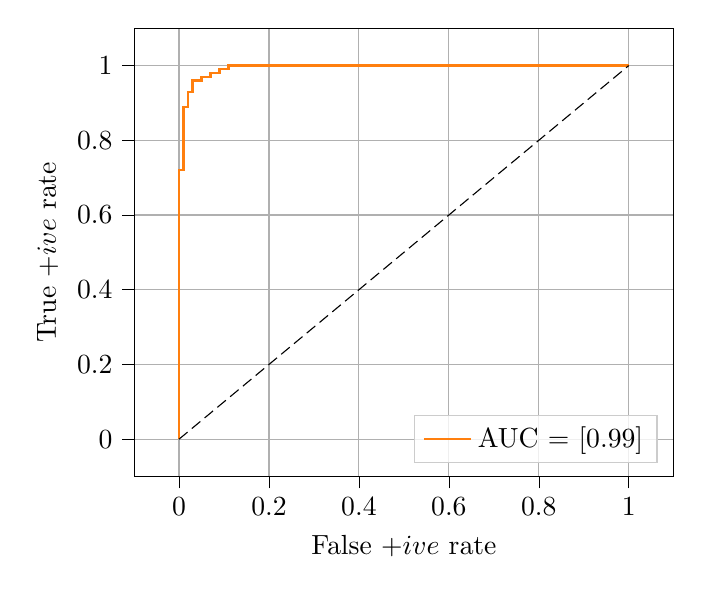
\begin{tikzpicture}
  \begin{axis}
    [
    ylabel={True $+ive$ rate},
    xlabel={False $+ive$ rate},
    tick align=outside,
    tick pos=left,
    ytick style={color=black},
    xtick style={color=black},
    grid style={gridgrey},
    xmajorgrids,
    ymajorgrids,
    legend cell align={left},
    legend columns=1,
    legend style={
      fill opacity=0.8,
      draw opacity=1,
      text opacity=1,
      at={(0.97,0.03)},
      anchor=south east,
      draw=legendgray,
    },
    ]
    \addlegendentry{AUC = $[0.99]$}
    \addplot[thick, darkorange] table {
      0.0 0.0
      0.0 0.01
      0.0 0.03
      0.0 0.05
      0.0 0.12
      0.0 0.14
      0.0 0.27
      0.0 0.29
      0.0 0.32
      0.0 0.34
      0.0 0.42
      0.0 0.46
      0.0 0.51
      0.0 0.53
      0.0 0.54
      0.0 0.56
      0.0 0.64
      0.0 0.66
      0.0 0.68
      0.0 0.7
      0.0 0.72
      0.01 0.72
      0.01 0.89
      0.02 0.89
      0.02 0.93
      0.03 0.93
      0.03 0.94
      0.03 0.96
      0.05 0.96
      0.05 0.97
      0.07 0.97
      0.07 0.98
      0.09 0.98
      0.09 0.99
      0.11 0.99
      0.11 1.0
      1.0 1.0
    };
    \addplot[black, dashed, dash pattern=on 4pt off 2pt] table {
      0 0
      1 1
    };
  \end{axis}
\end{tikzpicture}
}
              \captionsetup{justification=centering}
              \caption{With data leak}
            \end{subfigure}%
            \hspace{0.05\textwidth}
            \begin{subfigure}{0.45\textwidth}
              \centering
              \resizebox{\textwidth}{!}{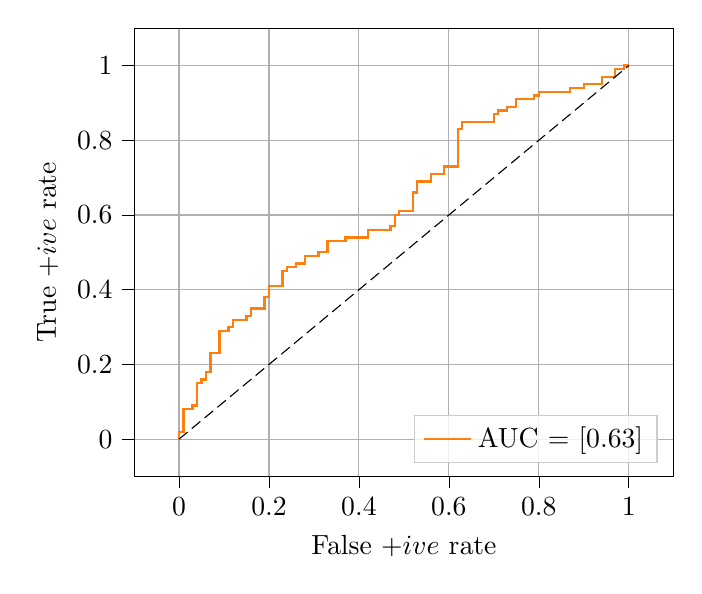
\begin{tikzpicture}
  \begin{axis}
    [
    ylabel={True $+ive$ rate},
    xlabel={False $+ive$ rate},
    tick align=outside,
    tick pos=left,
    ytick style={color=black},
    xtick style={color=black},
    grid style={gridgrey},
    xmajorgrids,
    ymajorgrids,
    legend cell align={left},
    legend columns=1,
    legend style={
      fill opacity=0.8,
      draw opacity=1,
      text opacity=1,
      at={(0.97,0.03)},
      anchor=south east,
      draw=legendgray,
    },
    ]
    \addlegendentry{AUC = $[0.63]$}
    \addplot[thick, darkorange] table {
      0.0 0.0
      0.0 0.01
      0.0 0.02
      0.01 0.02
      0.01 0.08
      0.03 0.08
      0.03 0.09
      0.04 0.09
      0.04 0.12
      0.04 0.14
      0.04 0.15
      0.05 0.15
      0.05 0.16
      0.06 0.16
      0.06 0.18
      0.07 0.18
      0.07 0.2
      0.07 0.23
      0.09 0.23
      0.09 0.25
      0.09 0.27
      0.09 0.29
      0.11 0.29
      0.11 0.3
      0.12 0.3
      0.12 0.32
      0.15 0.32
      0.15 0.33
      0.16 0.33
      0.16 0.35
      0.19 0.35
      0.19 0.36
      0.19 0.38
      0.2 0.38
      0.2 0.4
      0.2 0.41
      0.23 0.41
      0.23 0.43
      0.23 0.45
      0.24 0.45
      0.24 0.46
      0.26 0.46
      0.26 0.47
      0.28 0.47
      0.28 0.49
      0.31 0.49
      0.31 0.5
      0.33 0.5
      0.33 0.53
      0.37 0.53
      0.37 0.54
      0.42 0.54
      0.42 0.56
      0.47 0.56
      0.47 0.57
      0.48 0.57
      0.48 0.58
      0.48 0.6
      0.49 0.6
      0.49 0.61
      0.52 0.61
      0.52 0.66
      0.53 0.66
      0.53 0.69
      0.56 0.69
      0.56 0.71
      0.59 0.71
      0.59 0.73
      0.62 0.73
      0.62 0.83
      0.63 0.83
      0.63 0.85
      0.7 0.85
      0.7 0.87
      0.71 0.87
      0.71 0.88
      0.73 0.88
      0.73 0.89
      0.75 0.89
      0.75 0.91
      0.79 0.91
      0.79 0.92
      0.8 0.92
      0.8 0.93
      0.87 0.93
      0.87 0.94
      0.9 0.94
      0.9 0.95
      0.94 0.95
      0.94 0.97
      0.97 0.97
      0.97 0.99
      0.99 0.99
      0.99 1.0
      1.0 1.0
    };
    \addplot[black, dashed, dash pattern=on 4pt off 2pt] table {
      0 0
      1 1
    };
  \end{axis}
\end{tikzpicture}
}
              \captionsetup{justification=centering}
              \caption{Without data leak}
            \end{subfigure}
            \caption{XGBoost results on \textbf{S\_200} dataset}\label{fig:xgb_s200}
        \end{figure}

      \paragraph{Mus musculus}
        \noindent
        \begin{table}[H]
            \centering
            \begin{tabular}{lcc}
              \toprule
              \textbf{Metric} & \textbf{Data Leak} & \textbf{Fixed} \\
              \midrule
              Accuracy        & 99\%               & 61\%           \\
              MCC             & 0.98               & 0.23           \\
              Sensitivity     & 98\%               & 61\%           \\
              Specificity     & 99\%               & 62\%           \\
              \bottomrule
            \end{tabular}
            \caption{Results for M\_944 dataset}
            \label{tab:xgb_pstnpss_mm}
        \end{table}

        \begin{figure}[H]
            \centering
            \begin{subfigure}{0.47\textwidth}
              \centering
              \resizebox{\textwidth}{!}{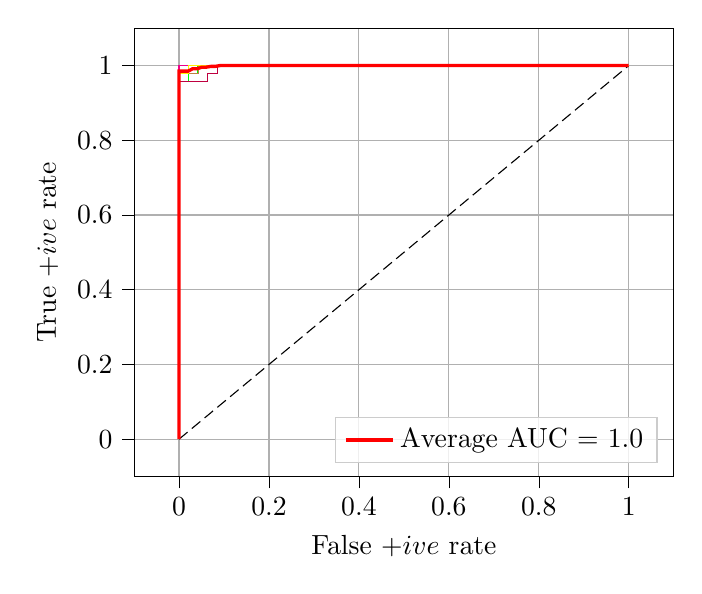
\begin{tikzpicture}
  \begin{axis}
    [
    ylabel={True $+ive$ rate},
    xlabel={False $+ive$ rate},
    tick align=outside,
    tick pos=left,
    ytick style={color=black},
    xtick style={color=black},
    grid style={gridgrey},
    xmajorgrids,
    ymajorgrids,
    legend cell align={left},
    legend columns=1,
    legend style={
      fill opacity=0.8,
      draw opacity=1,
      text opacity=1,
      at={(0.97,0.03)},
      anchor=south east,
      draw=legendgray,
    },
    ]

    \addplot[black, dashed, dash pattern=on 4pt off 2pt, forget plot] table {
      0 0
      1 1
    };


    \addplot[thin, color=steelblue, forget plot] table {
      0.0 0.0
      0.0 0.020833333333333332
      0.0 1.0
      1.0 1.0
    };


    \addplot[thin, color=darkorange, forget plot] table {
      0.0 0.0
      0.0 0.020833333333333332
      0.0 1.0
      1.0 1.0
    };


    \addplot[thin, color=green, forget plot] table {
      0.0 0.0
      0.0 0.02127659574468085
      0.0 0.9574468085106383
      0.020833333333333332 0.9574468085106383
      0.020833333333333332 0.9787234042553191
      0.041666666666666664 0.9787234042553191
      0.041666666666666664 1.0
      1.0 1.0
    };


    \addplot[thin, color=gray, forget plot] table {
      0.0 0.0
      0.0 0.02127659574468085
      0.0 0.9787234042553191
      0.020833333333333332 0.9787234042553191
      0.020833333333333332 1.0
      1.0 1.0
    };


    \addplot[thin, color=purple, forget plot] table {
      0.0 0.0
      0.0 0.02127659574468085
      0.0 0.9574468085106383
      0.06382978723404255 0.9574468085106383
      0.06382978723404255 0.9787234042553191
      0.0851063829787234 0.9787234042553191
      0.0851063829787234 1.0
      1.0 1.0
    };


    \addplot[thin, color=brown, forget plot] table {
      0.0 0.0
      0.0 0.02127659574468085
      0.0 0.9787234042553191
      0.0425531914893617 0.9787234042553191
      0.0425531914893617 1.0
      1.0 1.0
    };


    \addplot[thin, color=pink, forget plot] table {
      0.0 0.0
      0.0 0.02127659574468085
      0.0 1.0
      1.0 1.0
    };


    \addplot[thin, color=cyan, forget plot] table {
      0.0 0.0
      0.0 0.02127659574468085
      0.0 1.0
      1.0 1.0
    };


    \addplot[thin, color=magenta, forget plot] table {
      0.0 0.0
      0.0 0.02127659574468085
      0.0 1.0
      1.0 1.0
    };


    \addplot[thin, color=yellow, forget plot] table {
      0.0 0.0
      0.0 0.02127659574468085
      0.0 0.9787234042553191
      0.02127659574468085 0.9787234042553191
      0.02127659574468085 1.0
      1.0 1.0
    };

    \addlegendentry{Average AUC = $1.0$}
    \addplot[very thick, red] table {
      0 0
      0.0 0.9851063829787234
      0.010101010101010102 0.9851063829787234
      0.020202020202020204 0.9851063829787234
      0.030303030303030304 0.9914893617021278
      0.04040404040404041 0.9914893617021278
      0.05050505050505051 0.9957446808510639
      0.06060606060606061 0.9957446808510639
      0.07070707070707072 0.997872340425532
      0.08080808080808081 0.997872340425532
      0.09090909090909091 1.0
      0.10101010101010102 1.0
      0.11111111111111112 1.0
      0.12121212121212122 1.0
      0.13131313131313133 1.0
      0.14141414141414144 1.0
      0.15151515151515152 1.0
      0.16161616161616163 1.0
      0.17171717171717174 1.0
      0.18181818181818182 1.0
      0.19191919191919193 1.0
      0.20202020202020204 1.0
      0.21212121212121213 1.0
      0.22222222222222224 1.0
      0.23232323232323235 1.0
      0.24242424242424243 1.0
      0.25252525252525254 1.0
      0.26262626262626265 1.0
      0.27272727272727276 1.0
      0.2828282828282829 1.0
      0.29292929292929293 1.0
      0.30303030303030304 1.0
      0.31313131313131315 1.0
      0.32323232323232326 1.0
      0.33333333333333337 1.0
      0.3434343434343435 1.0
      0.3535353535353536 1.0
      0.36363636363636365 1.0
      0.37373737373737376 1.0
      0.38383838383838387 1.0
      0.393939393939394 1.0
      0.4040404040404041 1.0
      0.4141414141414142 1.0
      0.42424242424242425 1.0
      0.43434343434343436 1.0
      0.4444444444444445 1.0
      0.4545454545454546 1.0
      0.4646464646464647 1.0
      0.4747474747474748 1.0
      0.48484848484848486 1.0
      0.494949494949495 1.0
      0.5050505050505051 1.0
      0.5151515151515152 1.0
      0.5252525252525253 1.0
      0.5353535353535354 1.0
      0.5454545454545455 1.0
      0.5555555555555556 1.0
      0.5656565656565657 1.0
      0.5757575757575758 1.0
      0.5858585858585859 1.0
      0.595959595959596 1.0
      0.6060606060606061 1.0
      0.6161616161616162 1.0
      0.6262626262626263 1.0
      0.6363636363636365 1.0
      0.6464646464646465 1.0
      0.6565656565656566 1.0
      0.6666666666666667 1.0
      0.6767676767676768 1.0
      0.686868686868687 1.0
      0.696969696969697 1.0
      0.7070707070707072 1.0
      0.7171717171717172 1.0
      0.7272727272727273 1.0
      0.7373737373737375 1.0
      0.7474747474747475 1.0
      0.7575757575757577 1.0
      0.7676767676767677 1.0
      0.7777777777777778 1.0
      0.787878787878788 1.0
      0.797979797979798 1.0
      0.8080808080808082 1.0
      0.8181818181818182 1.0
      0.8282828282828284 1.0
      0.8383838383838385 1.0
      0.8484848484848485 1.0
      0.8585858585858587 1.0
      0.8686868686868687 1.0
      0.8787878787878789 1.0
      0.888888888888889 1.0
      0.8989898989898991 1.0
      0.9090909090909092 1.0
      0.9191919191919192 1.0
      0.9292929292929294 1.0
      0.9393939393939394 1.0
      0.9494949494949496 1.0
      0.9595959595959597 1.0
      0.9696969696969697 1.0
      0.9797979797979799 1.0
      0.98989898989899 1.0
      1.0 1.0
    };


  \end{axis}
\end{tikzpicture}
}
              \captionsetup{justification=centering}
              \caption{With data leak}
            \end{subfigure}%
            \hspace{0.05\textwidth}
            \begin{subfigure}{0.47\textwidth}
              \centering
              \resizebox{\textwidth}{!}{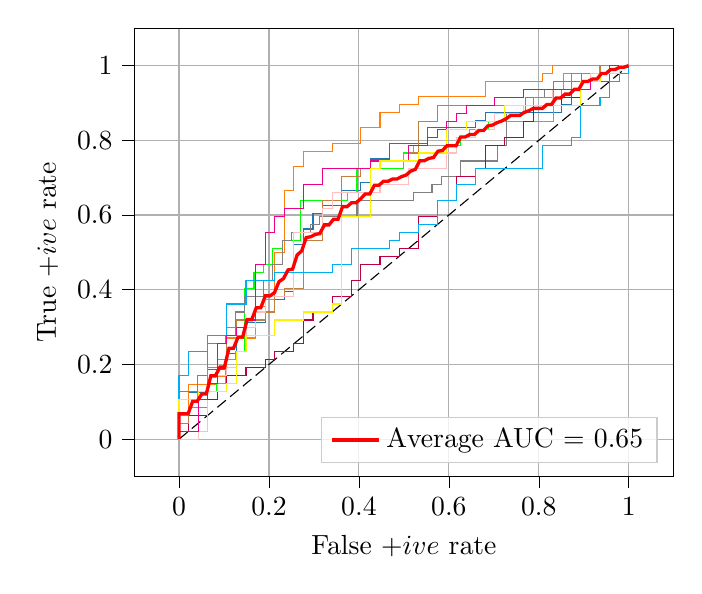
\begin{tikzpicture}
  \begin{axis}
    [
    ylabel={True $+ive$ rate},
    xlabel={False $+ive$ rate},
    tick align=outside,
    tick pos=left,
    ytick style={color=black},
    xtick style={color=black},
    grid style={gridgrey},
    xmajorgrids,
    ymajorgrids,
    legend cell align={left},
    legend columns=1,
    legend style={
      fill opacity=0.8,
      draw opacity=1,
      text opacity=1,
      at={(0.97,0.03)},
      anchor=south east,
      draw=legendgray,
    },
    ]

    \addplot[black, dashed, dash pattern=on 4pt off 2pt, forget plot] table {
      0 0
      1 1
    };


    \addplot[thin, color=steelblue, forget plot] table {
      0.0 0.0
      0.0 0.020833333333333332
      0.02127659574468085 0.020833333333333332
      0.02127659574468085 0.125
      0.06382978723404255 0.125
      0.06382978723404255 0.1875
      0.10638297872340426 0.1875
      0.10638297872340426 0.22916666666666666
      0.1276595744680851 0.22916666666666666
      0.1276595744680851 0.2708333333333333
      0.14893617021276595 0.2708333333333333
      0.14893617021276595 0.3125
      0.19148936170212766 0.3125
      0.19148936170212766 0.375
      0.23404255319148937 0.375
      0.23404255319148937 0.3958333333333333
      0.2553191489361702 0.3958333333333333
      0.2553191489361702 0.5208333333333334
      0.2765957446808511 0.5208333333333334
      0.2765957446808511 0.5625
      0.2978723404255319 0.5625
      0.2978723404255319 0.6041666666666666
      0.3191489361702128 0.6041666666666666
      0.3191489361702128 0.625
      0.3617021276595745 0.625
      0.3617021276595745 0.6666666666666666
      0.40425531914893614 0.6666666666666666
      0.40425531914893614 0.6875
      0.425531914893617 0.6875
      0.425531914893617 0.75
      0.46808510638297873 0.75
      0.46808510638297873 0.7916666666666666
      0.5531914893617021 0.7916666666666666
      0.5531914893617021 0.8333333333333334
      0.6595744680851063 0.8333333333333334
      0.6595744680851063 0.8541666666666666
      0.6808510638297872 0.8541666666666666
      0.6808510638297872 0.875
      0.851063829787234 0.875
      0.851063829787234 0.8958333333333334
      0.8723404255319149 0.8958333333333334
      0.8723404255319149 0.9583333333333334
      0.9574468085106383 0.9583333333333334
      0.9574468085106383 0.9791666666666666
      0.9787234042553191 0.9791666666666666
      0.9787234042553191 1.0
      1.0 1.0
    };


    \addplot[thin, color=darkorange, forget plot] table {
      0.0 0.0
      0.0 0.020833333333333332
      0.0 0.0625
      0.02127659574468085 0.0625
      0.02127659574468085 0.14583333333333334
      0.0851063829787234 0.14583333333333334
      0.0851063829787234 0.16666666666666666
      0.10638297872340426 0.16666666666666666
      0.10638297872340426 0.2708333333333333
      0.1702127659574468 0.2708333333333333
      0.1702127659574468 0.3541666666666667
      0.19148936170212766 0.3541666666666667
      0.19148936170212766 0.375
      0.2127659574468085 0.375
      0.2127659574468085 0.5
      0.23404255319148937 0.5
      0.23404255319148937 0.6666666666666666
      0.2553191489361702 0.6666666666666666
      0.2553191489361702 0.7291666666666666
      0.2765957446808511 0.7291666666666666
      0.2765957446808511 0.7708333333333334
      0.3404255319148936 0.7708333333333334
      0.3404255319148936 0.7916666666666666
      0.40425531914893614 0.7916666666666666
      0.40425531914893614 0.8333333333333334
      0.44680851063829785 0.8333333333333334
      0.44680851063829785 0.875
      0.48936170212765956 0.875
      0.48936170212765956 0.8958333333333334
      0.5319148936170213 0.8958333333333334
      0.5319148936170213 0.9166666666666666
      0.6808510638297872 0.9166666666666666
      0.6808510638297872 0.9583333333333334
      0.8085106382978723 0.9583333333333334
      0.8085106382978723 0.9791666666666666
      0.8297872340425532 0.9791666666666666
      0.8297872340425532 1.0
      1.0 1.0
    };


    \addplot[thin, color=green, forget plot] table {
      0.0 0.0
      0.0 0.02127659574468085
      0.0 0.10638297872340426
      0.041666666666666664 0.10638297872340426
      0.041666666666666664 0.1276595744680851
      0.08333333333333333 0.1276595744680851
      0.08333333333333333 0.14893617021276595
      0.10416666666666667 0.14893617021276595
      0.10416666666666667 0.2127659574468085
      0.125 0.2127659574468085
      0.125 0.23404255319148937
      0.14583333333333334 0.23404255319148937
      0.14583333333333334 0.40425531914893614
      0.16666666666666666 0.40425531914893614
      0.16666666666666666 0.44680851063829785
      0.1875 0.44680851063829785
      0.1875 0.46808510638297873
      0.20833333333333334 0.46808510638297873
      0.20833333333333334 0.5106382978723404
      0.22916666666666666 0.5106382978723404
      0.22916666666666666 0.5319148936170213
      0.2708333333333333 0.5319148936170213
      0.2708333333333333 0.6382978723404256
      0.375 0.6382978723404256
      0.375 0.6595744680851063
      0.3958333333333333 0.6595744680851063
      0.3958333333333333 0.723404255319149
      0.5 0.723404255319149
      0.5 0.7659574468085106
      0.5208333333333334 0.7659574468085106
      0.5208333333333334 0.7872340425531915
      0.625 0.7872340425531915
      0.625 0.8085106382978723
      0.6458333333333334 0.8085106382978723
      0.6458333333333334 0.8297872340425532
      0.6875 0.8297872340425532
      0.6875 0.851063829787234
      0.8333333333333334 0.851063829787234
      0.8333333333333334 0.9361702127659575
      0.8541666666666666 0.9361702127659575
      0.8541666666666666 0.9787234042553191
      1.0 0.9787234042553191
      1.0 1.0
    };


    \addplot[thin, color=gray, forget plot] table {
      0.0 0.0
      0.0 0.02127659574468085
      0.0 0.1276595744680851
      0.041666666666666664 0.1276595744680851
      0.041666666666666664 0.1702127659574468
      0.0625 0.1702127659574468
      0.0625 0.2553191489361702
      0.10416666666666667 0.2553191489361702
      0.10416666666666667 0.2765957446808511
      0.125 0.2765957446808511
      0.125 0.3404255319148936
      0.14583333333333334 0.3404255319148936
      0.14583333333333334 0.3829787234042553
      0.1875 0.3829787234042553
      0.1875 0.425531914893617
      0.20833333333333334 0.425531914893617
      0.20833333333333334 0.46808510638297873
      0.22916666666666666 0.46808510638297873
      0.22916666666666666 0.5319148936170213
      0.25 0.5319148936170213
      0.25 0.5531914893617021
      0.2916666666666667 0.5531914893617021
      0.2916666666666667 0.574468085106383
      0.3125 0.574468085106383
      0.3125 0.5957446808510638
      0.3958333333333333 0.5957446808510638
      0.3958333333333333 0.6382978723404256
      0.5208333333333334 0.6382978723404256
      0.5208333333333334 0.6595744680851063
      0.5625 0.6595744680851063
      0.5625 0.6808510638297872
      0.5833333333333334 0.6808510638297872
      0.5833333333333334 0.7021276595744681
      0.625 0.7021276595744681
      0.625 0.7446808510638298
      0.7083333333333334 0.7446808510638298
      0.7083333333333334 0.7872340425531915
      0.7291666666666666 0.7872340425531915
      0.7291666666666666 0.8723404255319149
      0.7708333333333334 0.8723404255319149
      0.7708333333333334 0.9148936170212766
      0.8125 0.9148936170212766
      0.8125 0.9361702127659575
      0.8333333333333334 0.9361702127659575
      0.8333333333333334 0.9574468085106383
      0.8958333333333334 0.9574468085106383
      0.8958333333333334 0.9787234042553191
      0.9375 0.9787234042553191
      0.9375 1.0
      1.0 1.0
    };


    \addplot[thin, color=purple, forget plot] table {
      0.0 0.0
      0.0 0.02127659574468085
      0.02127659574468085 0.02127659574468085
      0.02127659574468085 0.06382978723404255
      0.06382978723404255 0.06382978723404255
      0.06382978723404255 0.10638297872340426
      0.0851063829787234 0.10638297872340426
      0.0851063829787234 0.1276595744680851
      0.10638297872340426 0.1276595744680851
      0.10638297872340426 0.1702127659574468
      0.14893617021276595 0.1702127659574468
      0.14893617021276595 0.19148936170212766
      0.19148936170212766 0.19148936170212766
      0.19148936170212766 0.2127659574468085
      0.2127659574468085 0.2127659574468085
      0.2127659574468085 0.23404255319148937
      0.2553191489361702 0.23404255319148937
      0.2553191489361702 0.2553191489361702
      0.2765957446808511 0.2553191489361702
      0.2765957446808511 0.3191489361702128
      0.2978723404255319 0.3191489361702128
      0.2978723404255319 0.3404255319148936
      0.3404255319148936 0.3404255319148936
      0.3404255319148936 0.3829787234042553
      0.3829787234042553 0.3829787234042553
      0.3829787234042553 0.425531914893617
      0.40425531914893614 0.425531914893617
      0.40425531914893614 0.46808510638297873
      0.44680851063829785 0.46808510638297873
      0.44680851063829785 0.48936170212765956
      0.48936170212765956 0.48936170212765956
      0.48936170212765956 0.5106382978723404
      0.5319148936170213 0.5106382978723404
      0.5319148936170213 0.5957446808510638
      0.574468085106383 0.5957446808510638
      0.574468085106383 0.6382978723404256
      0.6170212765957447 0.6382978723404256
      0.6170212765957447 0.7021276595744681
      0.6595744680851063 0.7021276595744681
      0.6595744680851063 0.723404255319149
      0.6808510638297872 0.723404255319149
      0.6808510638297872 0.7872340425531915
      0.723404255319149 0.7872340425531915
      0.723404255319149 0.8085106382978723
      0.7659574468085106 0.8085106382978723
      0.7659574468085106 0.851063829787234
      0.7872340425531915 0.851063829787234
      0.7872340425531915 0.8936170212765957
      0.851063829787234 0.8936170212765957
      0.851063829787234 0.9148936170212766
      0.8936170212765957 0.9148936170212766
      0.8936170212765957 0.9361702127659575
      0.9148936170212766 0.9361702127659575
      0.9148936170212766 0.9574468085106383
      0.9361702127659575 0.9574468085106383
      0.9361702127659575 1.0
      1.0 1.0
    };


    \addplot[thin, color=brown, forget plot] table {
      0.0 0.0
      0.0 0.02127659574468085
      0.0 0.0425531914893617
      0.02127659574468085 0.0425531914893617
      0.02127659574468085 0.0851063829787234
      0.06382978723404255 0.0851063829787234
      0.06382978723404255 0.19148936170212766
      0.0851063829787234 0.19148936170212766
      0.0851063829787234 0.2127659574468085
      0.10638297872340426 0.2127659574468085
      0.10638297872340426 0.2978723404255319
      0.1276595744680851 0.2978723404255319
      0.1276595744680851 0.3191489361702128
      0.19148936170212766 0.3191489361702128
      0.19148936170212766 0.3404255319148936
      0.2127659574468085 0.3404255319148936
      0.2127659574468085 0.3829787234042553
      0.23404255319148937 0.3829787234042553
      0.23404255319148937 0.40425531914893614
      0.2765957446808511 0.40425531914893614
      0.2765957446808511 0.5319148936170213
      0.3191489361702128 0.5319148936170213
      0.3191489361702128 0.6382978723404256
      0.3617021276595745 0.6382978723404256
      0.3617021276595745 0.7021276595744681
      0.40425531914893614 0.7021276595744681
      0.40425531914893614 0.723404255319149
      0.425531914893617 0.723404255319149
      0.425531914893617 0.7446808510638298
      0.5106382978723404 0.7446808510638298
      0.5106382978723404 0.7659574468085106
      0.5319148936170213 0.7659574468085106
      0.5319148936170213 0.851063829787234
      0.574468085106383 0.851063829787234
      0.574468085106383 0.8936170212765957
      0.7872340425531915 0.8936170212765957
      0.7872340425531915 0.9148936170212766
      0.851063829787234 0.9148936170212766
      0.851063829787234 0.9361702127659575
      0.8723404255319149 0.9361702127659575
      0.8723404255319149 0.9787234042553191
      0.9361702127659575 0.9787234042553191
      0.9361702127659575 1.0
      1.0 1.0
    };


    \addplot[thin, color=pink, forget plot] table {
      0.0 0.0
      0.02127659574468085 0.0
      0.0425531914893617 0.0
      0.0425531914893617 0.02127659574468085
      0.06382978723404255 0.02127659574468085
      0.06382978723404255 0.1276595744680851
      0.0851063829787234 0.1276595744680851
      0.0851063829787234 0.1702127659574468
      0.10638297872340426 0.1702127659574468
      0.10638297872340426 0.19148936170212766
      0.1276595744680851 0.19148936170212766
      0.1276595744680851 0.23404255319148937
      0.14893617021276595 0.23404255319148937
      0.14893617021276595 0.2978723404255319
      0.1702127659574468 0.2978723404255319
      0.1702127659574468 0.3404255319148936
      0.19148936170212766 0.3404255319148936
      0.19148936170212766 0.3829787234042553
      0.2553191489361702 0.3829787234042553
      0.2553191489361702 0.5531914893617021
      0.3191489361702128 0.5531914893617021
      0.3191489361702128 0.6170212765957447
      0.3404255319148936 0.6170212765957447
      0.3404255319148936 0.6595744680851063
      0.44680851063829785 0.6595744680851063
      0.44680851063829785 0.6808510638297872
      0.5106382978723404 0.6808510638297872
      0.5106382978723404 0.723404255319149
      0.5957446808510638 0.723404255319149
      0.5957446808510638 0.7659574468085106
      0.6170212765957447 0.7659574468085106
      0.6170212765957447 0.8085106382978723
      0.6595744680851063 0.8085106382978723
      0.6595744680851063 0.8297872340425532
      0.7021276595744681 0.8297872340425532
      0.7021276595744681 0.8723404255319149
      0.7659574468085106 0.8723404255319149
      0.7659574468085106 0.8936170212765957
      0.8297872340425532 0.8936170212765957
      0.8297872340425532 0.9361702127659575
      0.8936170212765957 0.9361702127659575
      0.8936170212765957 0.9574468085106383
      0.9148936170212766 0.9574468085106383
      0.9148936170212766 0.9787234042553191
      0.9574468085106383 0.9787234042553191
      0.9574468085106383 1.0
      1.0 1.0
    };


    \addplot[thin, color=cyan, forget plot] table {
      0.0 0.0
      0.0 0.02127659574468085
      0.0 0.1702127659574468
      0.02127659574468085 0.1702127659574468
      0.02127659574468085 0.23404255319148937
      0.06382978723404255 0.23404255319148937
      0.06382978723404255 0.2765957446808511
      0.10638297872340426 0.2765957446808511
      0.10638297872340426 0.3617021276595745
      0.14893617021276595 0.3617021276595745
      0.14893617021276595 0.425531914893617
      0.2127659574468085 0.425531914893617
      0.2127659574468085 0.44680851063829785
      0.3404255319148936 0.44680851063829785
      0.3404255319148936 0.46808510638297873
      0.3829787234042553 0.46808510638297873
      0.3829787234042553 0.5106382978723404
      0.46808510638297873 0.5106382978723404
      0.46808510638297873 0.5319148936170213
      0.48936170212765956 0.5319148936170213
      0.48936170212765956 0.5531914893617021
      0.5319148936170213 0.5531914893617021
      0.5319148936170213 0.574468085106383
      0.574468085106383 0.574468085106383
      0.574468085106383 0.6382978723404256
      0.6170212765957447 0.6382978723404256
      0.6170212765957447 0.6808510638297872
      0.6595744680851063 0.6808510638297872
      0.6595744680851063 0.723404255319149
      0.8085106382978723 0.723404255319149
      0.8085106382978723 0.7872340425531915
      0.8723404255319149 0.7872340425531915
      0.8723404255319149 0.8085106382978723
      0.8936170212765957 0.8085106382978723
      0.8936170212765957 0.8936170212765957
      0.9361702127659575 0.8936170212765957
      0.9361702127659575 0.9148936170212766
      0.9574468085106383 0.9148936170212766
      0.9574468085106383 0.9574468085106383
      0.9787234042553191 0.9574468085106383
      0.9787234042553191 0.9787234042553191
      1.0 0.9787234042553191
      1.0 1.0
    };


    \addplot[thin, color=magenta, forget plot] table {
      0.0 0.0
      0.0 0.02127659574468085
      0.0425531914893617 0.02127659574468085
      0.0425531914893617 0.10638297872340426
      0.06382978723404255 0.10638297872340426
      0.06382978723404255 0.14893617021276595
      0.0851063829787234 0.14893617021276595
      0.0851063829787234 0.2553191489361702
      0.10638297872340426 0.2553191489361702
      0.10638297872340426 0.2765957446808511
      0.1276595744680851 0.2765957446808511
      0.1276595744680851 0.2978723404255319
      0.14893617021276595 0.2978723404255319
      0.14893617021276595 0.3191489361702128
      0.1702127659574468 0.3191489361702128
      0.1702127659574468 0.46808510638297873
      0.19148936170212766 0.46808510638297873
      0.19148936170212766 0.5531914893617021
      0.2127659574468085 0.5531914893617021
      0.2127659574468085 0.5957446808510638
      0.23404255319148937 0.5957446808510638
      0.23404255319148937 0.6170212765957447
      0.2765957446808511 0.6170212765957447
      0.2765957446808511 0.6808510638297872
      0.3191489361702128 0.6808510638297872
      0.3191489361702128 0.723404255319149
      0.425531914893617 0.723404255319149
      0.425531914893617 0.7446808510638298
      0.5106382978723404 0.7446808510638298
      0.5106382978723404 0.7872340425531915
      0.5531914893617021 0.7872340425531915
      0.5531914893617021 0.8085106382978723
      0.574468085106383 0.8085106382978723
      0.574468085106383 0.8297872340425532
      0.5957446808510638 0.8297872340425532
      0.5957446808510638 0.851063829787234
      0.6170212765957447 0.851063829787234
      0.6170212765957447 0.8723404255319149
      0.6382978723404256 0.8723404255319149
      0.6382978723404256 0.8936170212765957
      0.7021276595744681 0.8936170212765957
      0.7021276595744681 0.9148936170212766
      0.7659574468085106 0.9148936170212766
      0.7659574468085106 0.9361702127659575
      0.9148936170212766 0.9361702127659575
      0.9148936170212766 0.9574468085106383
      0.9361702127659575 0.9574468085106383
      0.9361702127659575 0.9787234042553191
      0.9574468085106383 0.9787234042553191
      0.9574468085106383 1.0
      1.0 1.0
    };


    \addplot[thin, color=yellow, forget plot] table {
      0.0 0.0
      0.0 0.02127659574468085
      0.0 0.10638297872340426
      0.0425531914893617 0.10638297872340426
      0.0425531914893617 0.1276595744680851
      0.10638297872340426 0.1276595744680851
      0.10638297872340426 0.14893617021276595
      0.1276595744680851 0.14893617021276595
      0.1276595744680851 0.23404255319148937
      0.14893617021276595 0.23404255319148937
      0.14893617021276595 0.2765957446808511
      0.2127659574468085 0.2765957446808511
      0.2127659574468085 0.3191489361702128
      0.2765957446808511 0.3191489361702128
      0.2765957446808511 0.3404255319148936
      0.3404255319148936 0.3404255319148936
      0.3404255319148936 0.3617021276595745
      0.3617021276595745 0.3617021276595745
      0.3617021276595745 0.5957446808510638
      0.425531914893617 0.5957446808510638
      0.425531914893617 0.723404255319149
      0.44680851063829785 0.723404255319149
      0.44680851063829785 0.7446808510638298
      0.5319148936170213 0.7446808510638298
      0.5319148936170213 0.7659574468085106
      0.5957446808510638 0.7659574468085106
      0.5957446808510638 0.8297872340425532
      0.6382978723404256 0.8297872340425532
      0.6382978723404256 0.851063829787234
      0.723404255319149 0.851063829787234
      0.723404255319149 0.8936170212765957
      0.8936170212765957 0.8936170212765957
      0.8936170212765957 0.9574468085106383
      0.9361702127659575 0.9574468085106383
      0.9361702127659575 0.9787234042553191
      0.9787234042553191 0.9787234042553191
      0.9787234042553191 1.0
      1.0 1.0
    };

    \addlegendentry{Average AUC = $0.65$}
    \addplot[very thick, red] table {
      0 0
      0.0 0.06790780141843972
      0.010101010101010102 0.06790780141843972
      0.020202020202020204 0.06790780141843972
      0.030303030303030304 0.10155141843971631
      0.04040404040404041 0.10155141843971631
      0.05050505050505051 0.12070035460992908
      0.06060606060606061 0.12070035460992908
      0.07070707070707072 0.16950354609929077
      0.08080808080808081 0.16950354609929077
      0.09090909090909091 0.19286347517730495
      0.10101010101010102 0.19286347517730495
      0.11111111111111112 0.24361702127659574
      0.12121212121212122 0.24361702127659574
      0.13131313131313133 0.27331560283687945
      0.14141414141414144 0.27331560283687945
      0.15151515151515152 0.3200354609929078
      0.16161616161616163 0.3200354609929078
      0.17171717171717174 0.3517730496453901
      0.18181818181818182 0.3517730496453901
      0.19191919191919193 0.38351063829787235
      0.20202020202020204 0.38351063829787235
      0.21212121212121213 0.3920212765957447
      0.22222222222222224 0.4215425531914893
      0.23232323232323235 0.4300531914893617
      0.24242424242424243 0.45305851063829783
      0.25252525252525254 0.45518617021276586
      0.26262626262626265 0.49308510638297876
      0.27272727272727276 0.5037234042553191
      0.2828282828282829 0.5397163120567375
      0.29292929292929293 0.5418439716312057
      0.30303030303030304 0.5481382978723404
      0.31313131313131315 0.5502659574468084
      0.32323232323232326 0.5736258865248227
      0.33333333333333337 0.5736258865248227
      0.3434343434343435 0.5884751773049647
      0.3535353535353536 0.5884751773049647
      0.36363636363636365 0.6224290780141845
      0.37373737373737376 0.6224290780141845
      0.38383838383838387 0.6330673758865248
      0.393939393939394 0.6330673758865248
      0.4040404040404041 0.6437056737588653
      0.4141414141414142 0.6563386524822695
      0.42424242424242425 0.6563386524822695
      0.43434343434343436 0.6796099290780141
      0.4444444444444445 0.6796099290780141
      0.4545454545454546 0.6901595744680852
      0.4646464646464647 0.6901595744680852
      0.4747474747474748 0.6964539007092199
      0.48484848484848486 0.6964539007092199
      0.494949494949495 0.7027925531914894
      0.5050505050505051 0.7070478723404255
      0.5151515151515152 0.7176861702127659
      0.5252525252525253 0.7219414893617022
      0.5353535353535354 0.7453014184397164
      0.5454545454545455 0.7453014184397164
      0.5555555555555556 0.751595744680851
      0.5656565656565657 0.7537234042553191
      0.5757575757575758 0.7707446808510638
      0.5858585858585859 0.7728723404255319
      0.595959595959596 0.7856382978723404
      0.6060606060606061 0.7856382978723404
      0.6161616161616162 0.7856382978723404
      0.6262626262626263 0.8090425531914894
      0.6363636363636365 0.8090425531914894
      0.6464646464646465 0.8154255319148935
      0.6565656565656566 0.8154255319148935
      0.6666666666666667 0.8260195035460992
      0.6767676767676768 0.8260195035460992
      0.686868686868687 0.8386524822695035
      0.696969696969697 0.8407801418439715
      0.7070707070707072 0.847163120567376
      0.7171717171717172 0.851418439716312
      0.7272727272727273 0.8578014184397164
      0.7373737373737375 0.8663120567375888
      0.7474747474747475 0.8663120567375888
      0.7575757575757577 0.8663120567375888
      0.7676767676767677 0.874822695035461
      0.7777777777777778 0.8790780141843971
      0.787878787878788 0.8854609929078014
      0.797979797979798 0.8854609929078014
      0.8080808080808082 0.8854609929078014
      0.8181818181818182 0.896054964539007
      0.8282828282828284 0.896054964539007
      0.8383838383838385 0.9130319148936172
      0.8484848484848485 0.9130319148936172
      0.8585858585858587 0.9236258865248226
      0.8686868686868687 0.9236258865248226
      0.8787878787878789 0.936258865248227
      0.888888888888889 0.936258865248227
      0.8989898989898991 0.9575354609929079
      0.9090909090909092 0.9575354609929079
      0.9191919191919192 0.9639184397163122
      0.9292929292929294 0.9639184397163122
      0.9393939393939394 0.9788120567375888
      0.9494949494949496 0.9788120567375888
      0.9595959595959597 0.9894060283687942
      0.9696969696969697 0.9894060283687942
      0.9797979797979799 0.9957446808510639
      0.98989898989899 0.9957446808510639
      1.0 1.0
    };


  \end{axis}
\end{tikzpicture}
}
              \captionsetup{justification=centering}
              \caption{Without data leak}
            \end{subfigure}
            \caption{XGBoost results on \textbf{H\_944} dataset}\label{fig:xgb_m944}
        \end{figure}

    \subsubsection{Porpoise}
      This study~\cite{li_porpoise_2021} uses stacked ensemble along with combination of different encoding schemes and feeds different feature sub sects to each predictor in the stacked model.
      However, the way they utilize PSTNPss is not described clearly, based on the provided code it is clear that they used external data for calculation the positive and negative matrices and then evaluated the performance on the same dataset, ideally the creation of dataset should be done by using the benchmark training set only because that way the results would be unbiased and will be comparable to other past researches.
      If we are to incorporate additional data then other models performance should also be checked with additional data to make the comparison fair.

      This following code snippet is from the official repository provided by the Authors,
      \begin{lstlisting}[caption={Porpoise PSTNPss implementation \(lines 39\textminus{61}\)},label={lst:porpoise-pstnpss}]
if typ == 'H':
    matrix_po = np.fromfile(father_path+'/'+'H_po.bin', dtype=float)
    matrix_po = matrix_po.reshape(19, 64)
    matrix_ne = np.fromfile(father_path + '/' + 'H_ne.bin', dtype=float)
    matrix_ne = matrix_ne.reshape(19, 64)
    positive_number = 4327
    negative_number = 3732

elif typ == 'S':
    matrix_po = np.fromfile(father_path + '/' + 'S_po.bin', dtype=float)
    matrix_po = matrix_po.reshape(29, 64)
    matrix_ne = np.fromfile(father_path + '/' + 'S_ne.bin', dtype=float)
    matrix_ne = matrix_ne.reshape(29, 64)
    positive_number = 1147
    negative_number = 1147

elif typ == 'M':
    matrix_po = np.fromfile(father_path + '/' + 'M_po.bin', dtype=float)
    matrix_po = matrix_po.reshape(19, 64)
    matrix_ne = np.fromfile(father_path + '/' + 'M_ne.bin', dtype=float)
    matrix_ne = matrix_ne.reshape(19, 64)
    positive_number = 3174
    negative_number = 3174
      \end{lstlisting}

      We can clearly see that we have six pre-calculated matrices (from .bin files), two for each species, and we do not know the source samples that were used in this calculation, after that we can see the number of positive and negative samples that are much higher compared to our dataset and in case of Homo Sapines, the number do not match it seems like the number of positive samples use is much higher then negative and hence it will be a bit biased.
      Since all the other models from past works are solely trained using the available data hence, we re-evaluated the performance using the standard implementation and here are the results.

      \paragraph{Homo sapiens}
        \noindent
        \begin{table}[H]
            \centering
            \begin{minipage}{0.45\textwidth}
              \centering
              \begin{tabular}{lcc}
                \toprule
                \textbf{Metric} & \textbf{Original} & \textbf{Fixed} \\
                \midrule
                Accuracy        & 73\%              & 57\%           \\
                MCC             & 0.58              & 0.14           \\
                Sensitivity     & 89\%              & 62\%           \\
                Specificity     & 68\%              & 52\%           \\
                \bottomrule
              \end{tabular}
              \caption{Results for H\_990 dataset}
            \end{minipage}%
            \hfill
            \begin{minipage}{0.45\textwidth}
              \centering
              \begin{tabular}{lcc}
                \toprule
                \textbf{Metric} & \textbf{Original} & \textbf{Fixed} \\
                \midrule
                Accuracy        & 77\%              & 63\%           \\
                MCC             & 0.55              & 0.27           \\
                Sensitivity     & 82\%              & 73\%           \\
                Specificity     & 72\%              & 53\%           \\
                \bottomrule
              \end{tabular}
              \caption{Results for H\_200 dataset}
            \end{minipage}\label{tab:porpoise_pstnpss_hs}
        \end{table}

        \begin{figure}[H]
            \centering
            \begin{subfigure}{0.47\textwidth}
              \centering
              \resizebox{\textwidth}{!}{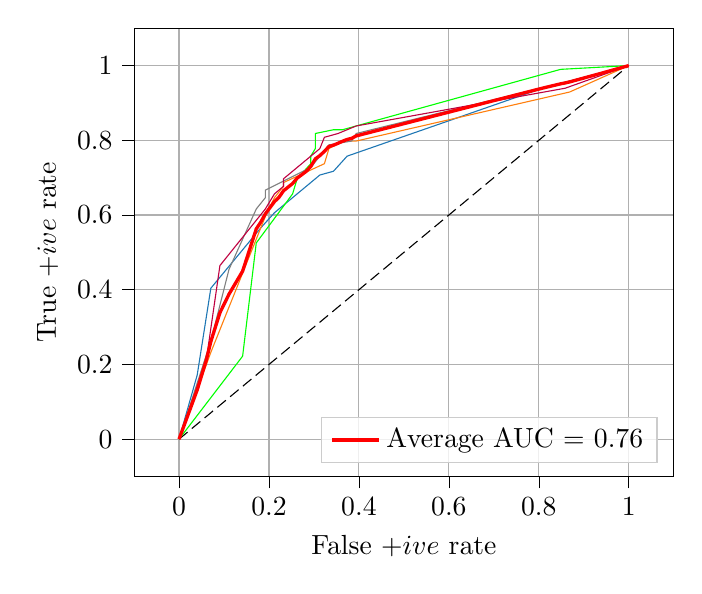
\begin{tikzpicture}
  \begin{axis}
    [
    ylabel={True $+ive$ rate},
    xlabel={False $+ive$ rate},
    tick align=outside,
    tick pos=left,
    ytick style={color=black},
    xtick style={color=black},
    grid style={gridgrey},
    xmajorgrids,
    ymajorgrids,
    legend cell align={left},
    legend columns=1,
    legend style={
      fill opacity=0.8,
      draw opacity=1,
      text opacity=1,
      at={(0.97,0.03)},
      anchor=south east,
      draw=legendgray,
    },
    ]

    \addplot[black, dashed, dash pattern=on 4pt off 2pt, forget plot] table {
      0 0
      1 1
    };


    \addplot[thin, color=steelblue, forget plot] table {
      0.0 0.0
      0.04040404040404041 0.1717171717171717
      0.0707070707070707 0.40404040404040403
      0.18181818181818182 0.5656565656565656
      0.21212121212121213 0.6060606060606061
      0.2222222222222222 0.6161616161616161
      0.24242424242424243 0.6363636363636364
      0.30303030303030304 0.696969696969697
      0.31313131313131315 0.7070707070707071
      0.3434343434343434 0.7171717171717171
      0.37373737373737376 0.7575757575757576
      0.8080808080808081 0.9393939393939394
      1.0 1.0
    };


    \addplot[thin, color=darkorange, forget plot] table {
      0.0 0.0
      0.0707070707070707 0.23232323232323232
      0.12121212121212122 0.3838383838383838
      0.1919191919191919 0.5959595959595959
      0.21212121212121213 0.6464646464646465
      0.23232323232323232 0.6767676767676768
      0.23232323232323232 0.6868686868686869
      0.32323232323232326 0.7373737373737373
      0.3333333333333333 0.7777777777777778
      0.36363636363636365 0.797979797979798
      0.3939393939393939 0.797979797979798
      0.8686868686868687 0.9292929292929293
      1.0 1.0
    };


    \addplot[thin, color=green, forget plot] table {
      0.0 0.0
      0.1414141414141414 0.2222222222222222
      0.1717171717171717 0.5252525252525253
      0.25252525252525254 0.6565656565656566
      0.26262626262626265 0.696969696969697
      0.29292929292929293 0.7373737373737373
      0.29292929292929293 0.7575757575757576
      0.30303030303030304 0.7777777777777778
      0.30303030303030304 0.8181818181818182
      0.3434343434343434 0.8282828282828283
      0.36363636363636365 0.8282828282828283
      0.8484848484848485 0.98989898989899
      1.0 1.0
    };


    \addplot[thin, color=gray, forget plot] table {
      0.0 0.0
      0.0707070707070707 0.26262626262626265
      0.1111111111111111 0.45454545454545453
      0.1717171717171717 0.6161616161616161
      0.1919191919191919 0.6464646464646465
      0.1919191919191919 0.6666666666666666
      0.29292929292929293 0.7272727272727273
      0.3333333333333333 0.7878787878787878
      0.3838383838383838 0.797979797979798
      0.3939393939393939 0.8181818181818182
      0.9393939393939394 0.9797979797979798
      1.0 1.0
    };


    \addplot[thin, color=purple, forget plot] table {
      0.0 0.0
      0.06060606060606061 0.21212121212121213
      0.09090909090909091 0.46464646464646464
      0.1919191919191919 0.6161616161616161
      0.21212121212121213 0.6565656565656566
      0.23232323232323232 0.6767676767676768
      0.23232323232323232 0.696969696969697
      0.31313131313131315 0.7777777777777778
      0.32323232323232326 0.8080808080808081
      0.35353535353535354 0.8181818181818182
      0.3939393939393939 0.8383838383838383
      0.8585858585858586 0.9393939393939394
      1.0 1.0
    };

    \addlegendentry{Average AUC = $0.76$}
    \addplot[very thick, red] table {
      0 0
      0.0 0.0
      0.010101010101010102 0.03297258297258297
      0.020202020202020204 0.06594516594516595
      0.030303030303030304 0.09891774891774892
      0.04040404040404041 0.1318903318903319
      0.05050505050505051 0.1717652717652718
      0.06060606060606061 0.21164021164021163
      0.07070707070707072 0.26127946127946133
      0.08080808080808081 0.2998841226113954
      0.09090909090909091 0.3384887839433294
      0.10101010101010102 0.36328873147054963
      0.11111111111111112 0.38808867899776994
      0.12121212121212122 0.4086798723162359
      0.13131313131313133 0.42927106563470196
      0.14141414141414144 0.4498622589531681
      0.15151515151515152 0.4874808692990511
      0.16161616161616163 0.5250994796449342
      0.17171717171717174 0.5627180899908172
      0.18181818181818182 0.581060606060606
      0.19191919191919193 0.6031986531986533
      0.20202020202020204 0.6194781144781146
      0.21212121212121213 0.6357575757575757
      0.22222222222222224 0.6473232323232324
      0.23232323232323235 0.664949494949495
      0.24242424242424243 0.6746071829405162
      0.25252525252525254 0.6842648709315375
      0.26262626262626265 0.6987205387205387
      0.27272727272727276 0.7077890011223346
      0.2828282828282829 0.7168574635241302
      0.29292929292929293 0.7299663299663302
      0.30303030303030304 0.750280583613917
      0.31313131313131315 0.7589786756453423
      0.32323232323232326 0.7703703703703704
      0.33333333333333337 0.7833333333333334
      0.3434343434343435 0.7869360269360269
      0.3535353535353536 0.7920538720538721
      0.36363636363636365 0.7975084175084175
      0.37373737373737376 0.8022895622895622
      0.38383838383838387 0.8052227703390494
      0.393939393939394 0.8117923420249001
      0.4040404040404041 0.8149079406710035
      0.4141414141414142 0.8180235393171067
      0.42424242424242425 0.8211391379632099
      0.43434343434343436 0.8242547366093131
      0.4444444444444445 0.8273703352554163
      0.4545454545454546 0.8304859339015195
      0.4646464646464647 0.8336015325476229
      0.4747474747474748 0.836717131193726
      0.48484848484848486 0.8398327298398293
      0.494949494949495 0.8429483284859325
      0.5050505050505051 0.8460639271320357
      0.5151515151515152 0.8491795257781389
      0.5252525252525253 0.852295124424242
      0.5353535353535354 0.8554107230703453
      0.5454545454545455 0.8585263217164485
      0.5555555555555556 0.8616419203625518
      0.5656565656565657 0.864757519008655
      0.5757575757575758 0.8678731176547583
      0.5858585858585859 0.8709887163008615
      0.595959595959596 0.8741043149469647
      0.6060606060606061 0.8772199135930678
      0.6161616161616162 0.8803355122391713
      0.6262626262626263 0.8834511108852745
      0.6363636363636365 0.8865667095313776
      0.6464646464646465 0.8896823081774808
      0.6565656565656566 0.8927979068235843
      0.6666666666666667 0.8959135054696873
      0.6767676767676768 0.8990291041157906
      0.686868686868687 0.9021447027618936
      0.696969696969697 0.9052603014079971
      0.7070707070707072 0.9083759000541003
      0.7171717171717172 0.9114914987002034
      0.7272727272727273 0.9146070973463066
      0.7373737373737375 0.9177226959924099
      0.7474747474747475 0.9208382946385132
      0.7575757575757577 0.9239538932846164
      0.7676767676767677 0.9270694919307196
      0.7777777777777778 0.9301850905768229
      0.787878787878788 0.9333006892229261
      0.797979797979798 0.9364162878690292
      0.8080808080808082 0.9395318865151324
      0.8181818181818182 0.9424397777319861
      0.8282828282828284 0.9453476689488397
      0.8383838383838385 0.9482555601656932
      0.8484848484848485 0.9511634513825469
      0.8585858585858587 0.9535326220606798
      0.8686868686868687 0.9563284192523959
      0.8787878787878789 0.9596532382497296
      0.888888888888889 0.9629780572470631
      0.8989898989898991 0.9663028762443968
      0.9090909090909092 0.9696276952417303
      0.9191919191919192 0.972952514239064
      0.9292929292929294 0.9762773332363975
      0.9393939393939394 0.979602152233731
      0.9494949494949496 0.9830017935281093
      0.9595959595959597 0.9864014348224874
      0.9696969696969697 0.9898010761168654
      0.9797979797979799 0.9932007174112438
      0.98989898989899 0.9966003587056219
      1.0 1.0
    };


  \end{axis}
\end{tikzpicture}
}
              \captionsetup{justification=centering}
              \caption{With data leak}
            \end{subfigure}%
            \hspace{0.05\textwidth}
            \begin{subfigure}{0.47\textwidth}
              \centering
              \resizebox{\textwidth}{!}{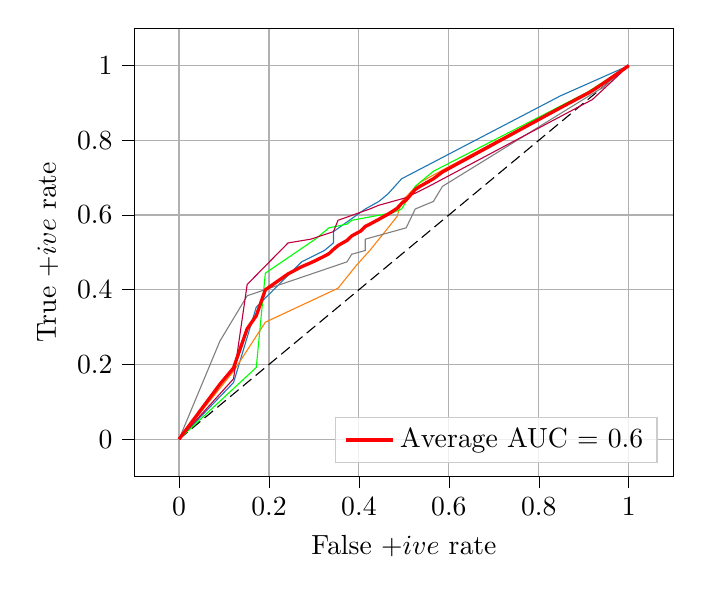
\begin{tikzpicture}
  \begin{axis}
    [
    ylabel={True $+ive$ rate},
    xlabel={False $+ive$ rate},
    tick align=outside,
    tick pos=left,
    ytick style={color=black},
    xtick style={color=black},
    grid style={gridgrey},
    xmajorgrids,
    ymajorgrids,
    legend cell align={left},
    legend columns=1,
    legend style={
      fill opacity=0.8,
      draw opacity=1,
      text opacity=1,
      at={(0.97,0.03)},
      anchor=south east,
      draw=legendgray,
    },
    ]

    \addplot[black, dashed, dash pattern=on 4pt off 2pt, forget plot] table {
      0 0
      1 1
    };


    \addplot[thin, color=steelblue, forget plot] table {
      0.0 0.0
      0.12121212121212122 0.15151515151515152
      0.1717171717171717 0.35353535353535354
      0.2727272727272727 0.47474747474747475
      0.32323232323232326 0.5050505050505051
      0.3434343434343434 0.5252525252525253
      0.3434343434343434 0.5555555555555556
      0.41414141414141414 0.6161616161616161
      0.4444444444444444 0.6363636363636364
      0.46464646464646464 0.6565656565656566
      0.494949494949495 0.696969696969697
      0.8484848484848485 0.9191919191919192
      1.0 1.0
    };


    \addplot[thin, color=darkorange, forget plot] table {
      0.0 0.0
      0.12121212121212122 0.18181818181818182
      0.1919191919191919 0.31313131313131315
      0.35353535353535354 0.40404040404040403
      0.3939393939393939 0.46464646464646464
      0.42424242424242425 0.5050505050505051
      0.48484848484848486 0.5959595959595959
      0.494949494949495 0.6363636363636364
      0.5353535353535354 0.6868686868686869
      0.5656565656565656 0.7070707070707071
      0.9090909090909091 0.9292929292929293
      1.0 1.0
    };


    \addplot[thin, color=green, forget plot] table {
      0.0 0.0
      0.1717171717171717 0.1919191919191919
      0.1919191919191919 0.4444444444444444
      0.30303030303030304 0.5353535353535354
      0.3333333333333333 0.5656565656565656
      0.37373737373737376 0.5757575757575758
      0.3838383838383838 0.5858585858585859
      0.47474747474747475 0.6060606060606061
      0.494949494949495 0.6161616161616161
      0.5252525252525253 0.6767676767676768
      0.5656565656565656 0.7171717171717171
      0.9090909090909091 0.9292929292929293
      1.0 1.0
    };


    \addplot[thin, color=gray, forget plot] table {
      0.0 0.0
      0.09090909090909091 0.26262626262626265
      0.15151515151515152 0.3838383838383838
      0.37373737373737376 0.47474747474747475
      0.3838383838383838 0.494949494949495
      0.41414141414141414 0.5050505050505051
      0.41414141414141414 0.5353535353535354
      0.5050505050505051 0.5656565656565656
      0.5252525252525253 0.6161616161616161
      0.5656565656565656 0.6363636363636364
      0.5858585858585859 0.6767676767676768
      0.9393939393939394 0.9393939393939394
      1.0 1.0
    };


    \addplot[thin, color=purple, forget plot] table {
      0.0 0.0
      0.12121212121212122 0.16161616161616163
      0.15151515151515152 0.41414141414141414
      0.24242424242424243 0.5252525252525253
      0.29292929292929293 0.5353535353535354
      0.3434343434343434 0.5555555555555556
      0.35353535353535354 0.5858585858585859
      0.42424242424242425 0.6161616161616161
      0.4444444444444444 0.6262626262626263
      0.5050505050505051 0.6464646464646465
      0.5555555555555556 0.6767676767676768
      0.9191919191919192 0.9090909090909091
      1.0 1.0
    };

    \addlegendentry{Average AUC = $0.6$}
    \addplot[very thick, red] table {
      0 0
      0.0 0.0
      0.010101010101010102 0.016343170264738895
      0.020202020202020204 0.03268634052947779
      0.030303030303030304 0.049029510794216684
      0.04040404040404041 0.06537268105895558
      0.05050505050505051 0.08171585132369448
      0.06060606060606061 0.09805902158843337
      0.07070707070707072 0.11440219185317228
      0.08080808080808081 0.13074536211791116
      0.09090909090909091 0.14708853238265004
      0.10101010101010102 0.1616359675183205
      0.11111111111111112 0.17618340265399088
      0.12121212121212122 0.19073083778966132
      0.13131313131313133 0.2256967433438022
      0.14141414141414144 0.26066264889794305
      0.15151515151515152 0.29562855445208386
      0.16161616161616163 0.3130146212142647
      0.17171717171717174 0.3304006879764457
      0.18181818181818182 0.3651248414884779
      0.19191919191919193 0.39984899500051013
      0.20202020202020204 0.4083580757065605
      0.21212121212121213 0.4168671564126109
      0.22222222222222224 0.4253762371186614
      0.23232323232323235 0.4338853178247118
      0.24242424242424243 0.4423943985307622
      0.25252525252525254 0.44883838383838387
      0.26262626262626265 0.45528236914600556
      0.27272727272727276 0.46172635445362725
      0.2828282828282829 0.46695821854912767
      0.29292929292929293 0.4721900826446281
      0.30303030303030304 0.47782598714416896
      0.31313131313131315 0.4838292011019284
      0.32323232323232326 0.4898324150596879
      0.33333333333333337 0.496643709825528
      0.3434343434343435 0.5080004591368229
      0.3535353535353536 0.5182605273514366
      0.36363636363636365 0.5252197297651844
      0.37373737373737376 0.5321789321789322
      0.38383838383838387 0.5438672438672438
      0.393939393939394 0.5506172839506174
      0.4040404040404041 0.5570306236972904
      0.4141414141414142 0.5695045695045695
      0.42424242424242425 0.5755331088664422
      0.43434343434343436 0.5820426487093153
      0.4444444444444445 0.5885521885521886
      0.4545454545454546 0.5953984287317622
      0.4646464646464647 0.6022446689113357
      0.4747474747474748 0.6097643097643098
      0.48484848484848486 0.6178451178451179
      0.494949494949495 0.6309764309764311
      0.5050505050505051 0.6401587301587301
      0.5151515151515152 0.6542568542568543
      0.5252525252525253 0.6683549783549785
      0.5353535353535354 0.6763924963924964
      0.5454545454545455 0.6832515632515633
      0.5555555555555556 0.6901106301106302
      0.5656565656565657 0.6970482603815938
      0.5757575757575758 0.7062041516943478
      0.5858585858585859 0.7153600430071018
      0.595959595959596 0.7219762517801736
      0.6060606060606061 0.7285924605532449
      0.6161616161616162 0.7352086693263165
      0.6262626262626263 0.7418248780993879
      0.6363636363636365 0.7484410868724595
      0.6464646464646465 0.7550572956455309
      0.6565656565656566 0.7616735044186024
      0.6666666666666667 0.7682897131916742
      0.6767676767676768 0.7749059219647456
      0.686868686868687 0.7815221307378171
      0.696969696969697 0.7881383395108885
      0.7070707070707072 0.7947545482839601
      0.7171717171717172 0.8013707570570316
      0.7272727272727273 0.8079869658301032
      0.7373737373737375 0.8146031746031748
      0.7474747474747475 0.8212193833762461
      0.7575757575757577 0.8278355921493177
      0.7676767676767677 0.8344518009223894
      0.7777777777777778 0.8410680096954607
      0.787878787878788 0.8476842184685323
      0.797979797979798 0.8543004272416036
      0.8080808080808082 0.8609166360146752
      0.8181818181818182 0.8675328447877467
      0.8282828282828284 0.8741490535608184
      0.8383838383838385 0.8807652623338897
      0.8484848484848485 0.8873814711069613
      0.8585858585858587 0.8938052796876328
      0.8686868686868687 0.900229088268304
      0.8787878787878789 0.9066528968489752
      0.888888888888889 0.9130767054296467
      0.8989898989898991 0.9195005140103181
      0.9090909090909092 0.9259243225909893
      0.9191919191919192 0.9329357062690397
      0.9292929292929294 0.9409291325957995
      0.9393939393939394 0.9489225589225591
      0.9494949494949496 0.9574354657687992
      0.9595959595959597 0.9659483726150395
      0.9696969696969697 0.9744612794612795
      0.9797979797979799 0.9829741863075198
      0.98989898989899 0.9914870931537598
      1.0 1.0
    };


  \end{axis}
\end{tikzpicture}
}
              \captionsetup{justification=centering}
              \caption{Without data leak}
            \end{subfigure}
            \caption{Porpoise results on \textbf{H\_990} dataset}\label{fig:porpoise_h990}
        \end{figure}

        \begin{figure}[H]
            \centering
            \begin{subfigure}{0.45\textwidth}
              \centering
              \resizebox{\textwidth}{!}{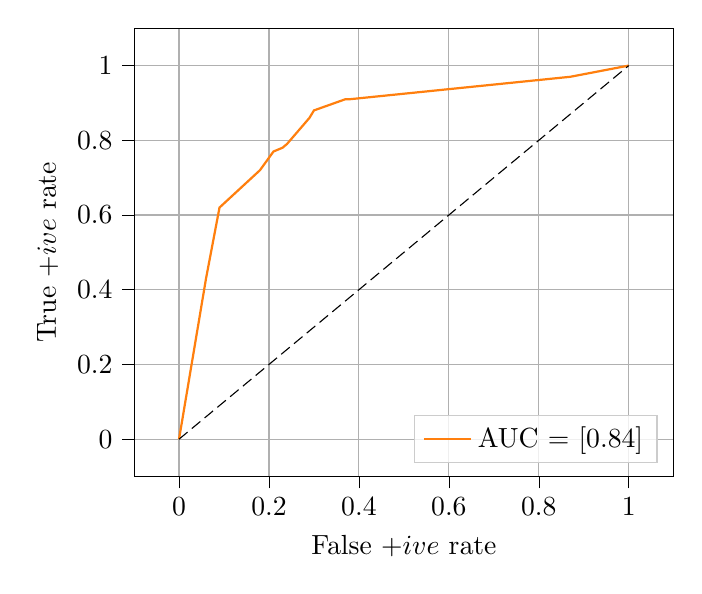
\begin{tikzpicture}
  \begin{axis}
    [
    ylabel={True $+ive$ rate},
    xlabel={False $+ive$ rate},
    tick align=outside,
    tick pos=left,
    ytick style={color=black},
    xtick style={color=black},
    grid style={gridgrey},
    xmajorgrids,
    ymajorgrids,
    legend cell align={left},
    legend columns=1,
    legend style={
      fill opacity=0.8,
      draw opacity=1,
      text opacity=1,
      at={(0.97,0.03)},
      anchor=south east,
      draw=legendgray,
    },
    ]
    \addlegendentry{AUC = $[0.84]$}
    \addplot[thick, darkorange] table {
      0.0 0.0
      0.06 0.43
      0.09 0.62
      0.18 0.72
      0.21 0.77
      0.23 0.78
      0.24 0.79
      0.29 0.86
      0.3 0.88
      0.37 0.91
      0.38 0.91
      0.87 0.97
      1.0 1.0
    };
    \addplot[black, dashed, dash pattern=on 4pt off 2pt] table {
      0 0
      1 1
    };
  \end{axis}
\end{tikzpicture}
}
              \captionsetup{justification=centering}
              \caption{With data leak}
            \end{subfigure}%
            \hspace{0.05\textwidth}
            \begin{subfigure}{0.45\textwidth}
              \centering
              \resizebox{\textwidth}{!}{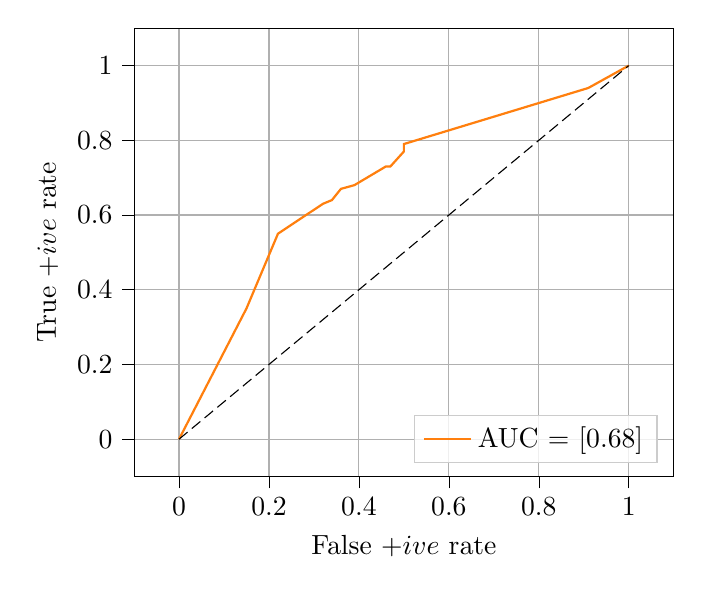
\begin{tikzpicture}
  \begin{axis}
    [
    ylabel={True $+ive$ rate},
    xlabel={False $+ive$ rate},
    tick align=outside,
    tick pos=left,
    ytick style={color=black},
    xtick style={color=black},
    grid style={gridgrey},
    xmajorgrids,
    ymajorgrids,
    legend cell align={left},
    legend columns=1,
    legend style={
      fill opacity=0.8,
      draw opacity=1,
      text opacity=1,
      at={(0.97,0.03)},
      anchor=south east,
      draw=legendgray,
    },
    ]
    \addlegendentry{AUC = $[0.68]$}
    \addplot[thick, darkorange] table {
      0.0 0.0
      0.15 0.35
      0.22 0.55
      0.32 0.63
      0.34 0.64
      0.36 0.67
      0.39 0.68
      0.46 0.73
      0.47 0.73
      0.5 0.77
      0.5 0.79
      0.91 0.94
      1.0 1.0
    };
    \addplot[black, dashed, dash pattern=on 4pt off 2pt] table {
      0 0
      1 1
    };
  \end{axis}
\end{tikzpicture}
}
              \captionsetup{justification=centering}
              \caption{Without data leak}
            \end{subfigure}
            \caption{Porpoise results on \textbf{H\_200} dataset}\label{fig:porpoise_h200}
        \end{figure}

      \paragraph{Saccharomyces cerevisiae}
        \noindent
        \begin{table}[H]
            \centering
            \begin{minipage}{0.45\textwidth}
              \centering
              \begin{tabular}{lcc}
                \toprule
                \textbf{Metric} & \textbf{Original} & \textbf{Fixed} \\
                \midrule
                Accuracy        & 82\%              & 65\%           \\
                MCC             & 0.63              & 0.31           \\
                Sensitivity     & 81\%              & 67\%           \\
                Specificity     & 82\%              & 64\%           \\
                \bottomrule
              \end{tabular}
              \caption{Results for S\_628 dataset}
            \end{minipage}%
            \hfill
            \begin{minipage}{0.45\textwidth}
              \centering
              \begin{tabular}{lcc}
                \toprule
                \textbf{Metric} & \textbf{Original} & \textbf{Fixed} \\
                \midrule
                Accuracy        & 83\%              & 68\%           \\
                MCC             & 0.67              & 0.35           \\
                Sensitivity     & 88\%              & 71\%           \\
                Specificity     & 79\%              & 64\%           \\
                \bottomrule
              \end{tabular}
              \caption{Results for S\_200 dataset}
            \end{minipage}\label{tab:porpoise_pstnpss_sc}
        \end{table}

        \begin{figure}[H]
            \centering
            \begin{subfigure}{0.47\textwidth}
              \centering
              \resizebox{\textwidth}{!}{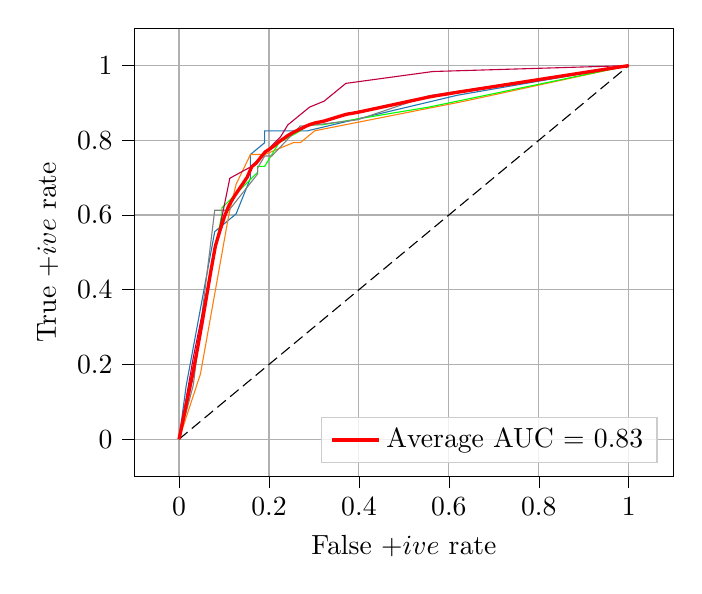
\begin{tikzpicture}
  \begin{axis}
    [
    ylabel={True $+ive$ rate},
    xlabel={False $+ive$ rate},
    tick align=outside,
    tick pos=left,
    ytick style={color=black},
    xtick style={color=black},
    grid style={gridgrey},
    xmajorgrids,
    ymajorgrids,
    legend cell align={left},
    legend columns=1,
    legend style={
      fill opacity=0.8,
      draw opacity=1,
      text opacity=1,
      at={(0.97,0.03)},
      anchor=south east,
      draw=legendgray,
    },
    ]

    \addplot[black, dashed, dash pattern=on 4pt off 2pt, forget plot] table {
      0 0
      1 1
    };


    \addplot[thin, color=steelblue, forget plot] table {
      0.0 0.0
      0.015873015873015872 0.14285714285714285
      0.07936507936507936 0.5555555555555556
      0.12698412698412698 0.6031746031746031
      0.15873015873015872 0.6984126984126984
      0.15873015873015872 0.7142857142857143
      0.15873015873015872 0.7619047619047619
      0.19047619047619047 0.7936507936507936
      0.19047619047619047 0.8253968253968254
      0.2222222222222222 0.8253968253968254
      0.2857142857142857 0.8253968253968254
      0.6190476190476191 0.9206349206349206
      1.0 1.0
    };


    \addplot[thin, color=darkorange, forget plot] table {
      0.0 0.0
      0.047619047619047616 0.1746031746031746
      0.1111111111111111 0.6031746031746031
      0.12698412698412698 0.6825396825396826
      0.15873015873015872 0.7619047619047619
      0.19047619047619047 0.7619047619047619
      0.25396825396825395 0.7936507936507936
      0.2698412698412698 0.7936507936507936
      0.30158730158730157 0.8253968253968254
      0.6349206349206349 0.9047619047619048
      1.0 1.0
    };


    \addplot[thin, color=green, forget plot] table {
      0.0 0.0
      0.015873015873015872 0.07936507936507936
      0.09523809523809523 0.6031746031746031
      0.09523809523809523 0.6190476190476191
      0.1746031746031746 0.7142857142857143
      0.1746031746031746 0.7301587301587301
      0.19047619047619047 0.7301587301587301
      0.2222222222222222 0.7936507936507936
      0.2698412698412698 0.8253968253968254
      0.2857142857142857 0.8412698412698413
      0.31746031746031744 0.8412698412698413
      0.5555555555555556 0.8888888888888888
      1.0 1.0
    };


    \addplot[thin, color=gray, forget plot] table {
      0.0 0.0
      0.031746031746031744 0.14516129032258066
      0.07936507936507936 0.6129032258064516
      0.1111111111111111 0.6129032258064516
      0.1746031746031746 0.7096774193548387
      0.1746031746031746 0.7258064516129032
      0.19047619047619047 0.7580645161290323
      0.20634920634920634 0.7580645161290323
      0.2698412698412698 0.8387096774193549
      0.2857142857142857 0.8387096774193549
      0.3968253968253968 0.8548387096774194
      0.5555555555555556 0.9193548387096774
      1.0 1.0
    };


    \addplot[thin, color=purple, forget plot] table {
      0.0 0.0
      0.03225806451612903 0.2222222222222222
      0.11290322580645161 0.6984126984126984
      0.16129032258064516 0.7301587301587301
      0.22580645161290322 0.8095238095238095
      0.24193548387096775 0.8412698412698413
      0.25806451612903225 0.8571428571428571
      0.2903225806451613 0.8888888888888888
      0.3225806451612903 0.9047619047619048
      0.3387096774193548 0.9206349206349206
      0.3709677419354839 0.9523809523809523
      0.5645161290322581 0.9841269841269841
      1.0 1.0
    };

    \addlegendentry{Average AUC = $0.83$}
    \addplot[very thick, red] table {
      0 0
      0.0 0.0
      0.010101010101010102 0.05884471959740778
      0.020202020202020204 0.11691021841559476
      0.030303030303030304 0.1739367561948207
      0.04040404040404041 0.23845086812828753
      0.05050505050505051 0.30587503297180724
      0.06060606060606061 0.3777484522645813
      0.07070707070707072 0.4496218715573555
      0.08080808080808081 0.5170731896538349
      0.09090909090909091 0.5579919005725457
      0.10101010101010102 0.5958514484320936
      0.11111111111111112 0.6258610684417136
      0.12121212121212122 0.6466923717461353
      0.13131313131313133 0.6652095282919656
      0.14141414141414144 0.6831494842605954
      0.15151515151515152 0.7010894402292253
      0.16161616161616163 0.7291678174473873
      0.17171717171717174 0.739176609929298
      0.18181818181818182 0.7545873481357352
      0.19191919191919193 0.7693938876734575
      0.20202020202020204 0.7769295618757983
      0.21212121212121213 0.7859315117379634
      0.22222222222222224 0.7960331683449964
      0.23232323232323235 0.8044032232204275
      0.24242424242424243 0.8132061785287592
      0.25252525252525254 0.8201171986118222
      0.26262626262626265 0.8261624178290845
      0.27272727272727276 0.8320997998417352
      0.2828282828282829 0.838128339203608
      0.29292929292929293 0.8430790976105875
      0.30303030303030304 0.8467439370665177
      0.31313131313131315 0.8490894609174179
      0.32323232323232326 0.851729998396665
      0.33333333333333337 0.8554736303123398
      0.3434343434343435 0.8592172622280149
      0.3535353535353536 0.8629608941436897
      0.36363636363636365 0.8667045260593648
      0.37373737373737376 0.8699938797429837
      0.38383838383838387 0.8720807322241015
      0.393939393939394 0.874167584705219
      0.4040404040404041 0.8766314794988631
      0.4141414141414142 0.8792461912175173
      0.42424242424242425 0.8818609029361717
      0.43434343434343436 0.8844756146548262
      0.4444444444444445 0.8870903263734805
      0.4545454545454546 0.8897050380921347
      0.4646464646464647 0.8923197498107891
      0.4747474747474748 0.8949344615294436
      0.48484848484848486 0.8975491732480979
      0.494949494949495 0.9001638849667524
      0.5050505050505051 0.9027785966854067
      0.5151515151515152 0.9053933084040612
      0.5252525252525253 0.9080080201227154
      0.5353535353535354 0.9106227318413698
      0.5454545454545455 0.9132374435600242
      0.5555555555555556 0.9158521552786786
      0.5656565656565657 0.9180842340838359
      0.5757575757575758 0.9200876892035794
      0.5858585858585859 0.9220911443233227
      0.595959595959596 0.9240945994430663
      0.6060606060606061 0.9260980545628097
      0.6161616161616162 0.9281015096825531
      0.6262626262626263 0.92999330397635
      0.6363636363636365 0.9318470066171484
      0.6464646464646465 0.9337401453222276
      0.6565656565656566 0.9356332840273067
      0.6666666666666667 0.9375264227323861
      0.6767676767676768 0.9394195614374652
      0.686868686868687 0.9413127001425444
      0.696969696969697 0.9432058388476235
      0.7070707070707072 0.9450989775527029
      0.7171717171717172 0.9469921162577821
      0.7272727272727273 0.9488852549628615
      0.7373737373737375 0.9507783936679406
      0.7474747474747475 0.9526715323730197
      0.7575757575757577 0.954564671078099
      0.7676767676767677 0.9564578097831783
      0.7777777777777778 0.9583509484882573
      0.787878787878788 0.9602440871933366
      0.797979797979798 0.9621372258984158
      0.8080808080808082 0.9640303646034949
      0.8181818181818182 0.9659235033085742
      0.8282828282828284 0.9678166420136535
      0.8383838383838385 0.9697097807187326
      0.8484848484848485 0.9716029194238118
      0.8585858585858587 0.9734960581288912
      0.8686868686868687 0.9753891968339703
      0.8787878787878789 0.9772823355390494
      0.888888888888889 0.9791754742441288
      0.8989898989898991 0.9810686129492078
      0.9090909090909092 0.9829617516542871
      0.9191919191919192 0.9848548903593664
      0.9292929292929294 0.9867480290644455
      0.9393939393939394 0.9886411677695248
      0.9494949494949496 0.9905343064746039
      0.9595959595959597 0.9924274451796832
      0.9696969696969697 0.9943205838847625
      0.9797979797979799 0.9962137225898416
      0.98989898989899 0.9981068612949209
      1.0 1.0
    };


  \end{axis}
\end{tikzpicture}
}
              \captionsetup{justification=centering}
              \caption{With data leak}
            \end{subfigure}%
            \hspace{0.05\textwidth}
            \begin{subfigure}{0.47\textwidth}
              \centering
              \resizebox{\textwidth}{!}{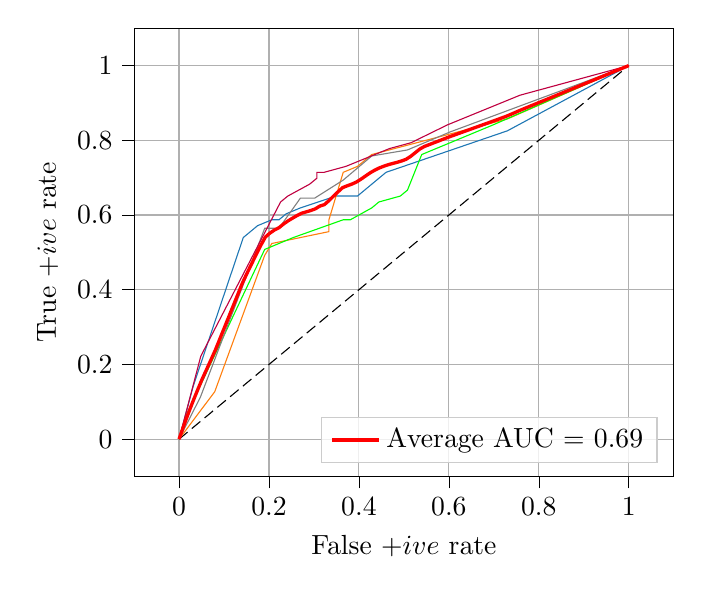
\begin{tikzpicture}
  \begin{axis}
    [
    ylabel={True $+ive$ rate},
    xlabel={False $+ive$ rate},
    tick align=outside,
    tick pos=left,
    ytick style={color=black},
    xtick style={color=black},
    grid style={gridgrey},
    xmajorgrids,
    ymajorgrids,
    legend cell align={left},
    legend columns=1,
    legend style={
      fill opacity=0.8,
      draw opacity=1,
      text opacity=1,
      at={(0.97,0.03)},
      anchor=south east,
      draw=legendgray,
    },
    ]

    \addplot[black, dashed, dash pattern=on 4pt off 2pt, forget plot] table {
      0 0
      1 1
    };


    \addplot[thin, color=steelblue, forget plot] table {
      0.0 0.0
      0.031746031746031744 0.14285714285714285
      0.14285714285714285 0.5396825396825397
      0.1746031746031746 0.5714285714285714
      0.20634920634920634 0.5873015873015873
      0.2222222222222222 0.5873015873015873
      0.23809523809523808 0.6031746031746031
      0.2698412698412698 0.6190476190476191
      0.3492063492063492 0.6507936507936508
      0.3968253968253968 0.6507936507936508
      0.4603174603174603 0.7142857142857143
      0.7301587301587301 0.8253968253968254
      1.0 1.0
    };


    \addplot[thin, color=darkorange, forget plot] table {
      0.0 0.0
      0.07936507936507936 0.12698412698412698
      0.19047619047619047 0.49206349206349204
      0.20634920634920634 0.5238095238095238
      0.3333333333333333 0.5555555555555556
      0.3333333333333333 0.5873015873015873
      0.36507936507936506 0.7142857142857143
      0.3968253968253968 0.7301587301587301
      0.42857142857142855 0.7619047619047619
      0.7301587301587301 0.8571428571428571
      1.0 1.0
    };


    \addplot[thin, color=green, forget plot] table {
      0.0 0.0
      0.015873015873015872 0.06349206349206349
      0.19047619047619047 0.5079365079365079
      0.25396825396825395 0.5396825396825397
      0.36507936507936506 0.5873015873015873
      0.38095238095238093 0.5873015873015873
      0.42857142857142855 0.6190476190476191
      0.4444444444444444 0.6349206349206349
      0.49206349206349204 0.6507936507936508
      0.5079365079365079 0.6666666666666666
      0.5396825396825397 0.7619047619047619
      0.6984126984126984 0.8412698412698413
      1.0 1.0
    };


    \addplot[thin, color=gray, forget plot] table {
      0.0 0.0
      0.047619047619047616 0.11290322580645161
      0.19047619047619047 0.5645161290322581
      0.2222222222222222 0.5645161290322581
      0.2698412698412698 0.6451612903225806
      0.30158730158730157 0.6451612903225806
      0.36507936507936506 0.6935483870967742
      0.4126984126984127 0.7419354838709677
      0.42857142857142855 0.7580645161290323
      0.5079365079365079 0.7741935483870968
      0.6031746031746031 0.8225806451612904
      1.0 1.0
    };


    \addplot[thin, color=purple, forget plot] table {
      0.0 0.0
      0.04838709677419355 0.2222222222222222
      0.22580645161290322 0.6349206349206349
      0.24193548387096775 0.6507936507936508
      0.2903225806451613 0.6825396825396826
      0.3064516129032258 0.6984126984126984
      0.3064516129032258 0.7142857142857143
      0.3225806451612903 0.7142857142857143
      0.3709677419354839 0.7301587301587301
      0.46774193548387094 0.7777777777777778
      0.5161290322580645 0.7936507936507936
      0.5967741935483871 0.8412698412698413
      0.7580645161290323 0.9206349206349206
      1.0 1.0
    };

    \addlegendentry{Average AUC = $0.69$}
    \addplot[very thick, red] table {
      0 0
      0.0 0.0
      0.010101010101010102 0.03447183905965269
      0.020202020202020204 0.0676843314054132
      0.030303030303030304 0.09921769479931748
      0.04040404040404041 0.12914314229959162
      0.05050505050505051 0.15829672094160296
      0.06060606060606061 0.1849720578417688
      0.07070707070707072 0.2116473947419346
      0.08080808080808081 0.23880922927145526
      0.09090909090909091 0.26889004957710444
      0.10101010101010102 0.29897086988275373
      0.11111111111111112 0.32905169018840297
      0.12121212121212122 0.3591325104940522
      0.13131313131313133 0.3892133307997015
      0.14141414141414144 0.41929415110535073
      0.15151515151515152 0.444922281244024
      0.16161616161616163 0.4698082963548681
      0.17171717171717174 0.49469431146571213
      0.18181818181818182 0.5188588258550555
      0.19191919191919193 0.5408610143703008
      0.20202020202020204 0.5516208493725601
      0.21212121212121213 0.5597832817774167
      0.22222222222222224 0.5659976622342213
      0.23232323232323235 0.5759044619259674
      0.24242424242424243 0.5843842935240785
      0.25252525252525254 0.5916562794698995
      0.26262626262626265 0.5988045795777491
      0.27272727272727276 0.6048970282150006
      0.2828282828282829 0.6084013839415785
      0.29292929292929293 0.6120767620614012
      0.30303030303030304 0.6164637709107755
      0.31313131313131315 0.6240302963805269
      0.32323232323232326 0.6277915736005854
      0.33333333333333337 0.6385220133453621
      0.3434343434343435 0.65047900431669
      0.3535353535353536 0.6620896749416976
      0.36363636363636365 0.6732385851049446
      0.37373737373737376 0.6781155125241146
      0.38383838383838387 0.6825572675035041
      0.393939393939394 0.6879610234448945
      0.4040404040404041 0.695529281550787
      0.4141414141414142 0.7039633405224803
      0.42424242424242425 0.7123973994941737
      0.43434343434343436 0.7194879890069478
      0.4444444444444445 0.7255709764255321
      0.4545454545454546 0.7303071624973153
      0.4646464646464647 0.7345340539421568
      0.4747474747474748 0.7378520745434869
      0.48484848484848486 0.7410685505988279
      0.494949494949495 0.7446698270389694
      0.5050505050505051 0.7492331044411118
      0.5151515151515152 0.7571222674272045
      0.5252525252525253 0.766820647347962
      0.5353535353535354 0.7765703339866927
      0.5454545454545455 0.7834340177394208
      0.5555555555555556 0.7881331993276465
      0.5656565656565657 0.7928323809158725
      0.5757575757575758 0.7975315625040982
      0.5858585858585859 0.8022307440923241
      0.595959595959596 0.8069299256805499
      0.6060606060606061 0.8114111364701596
      0.6161616161616162 0.8157883373708135
      0.6262626262626263 0.8201655382714673
      0.6363636363636365 0.824542739172121
      0.6464646464646465 0.8289199400727746
      0.6565656565656566 0.8332971409734287
      0.6666666666666667 0.8376743418740823
      0.6767676767676768 0.8420515427747359
      0.686868686868687 0.8464287436753898
      0.696969696969697 0.8508059445760434
      0.7070707070707072 0.8552287139433183
      0.7171717171717172 0.8596590780550301
      0.7272727272727273 0.8640894421667417
      0.7373737373737375 0.8691675933039494
      0.7474747474747475 0.8745048592513556
      0.7575757575757577 0.8798421251987616
      0.7676767676767677 0.8848640686086229
      0.7777777777777778 0.8898699786691175
      0.787878787878788 0.8948758887296122
      0.797979797979798 0.8998817987901069
      0.8080808080808082 0.9048877088506015
      0.8181818181818182 0.9098936189110962
      0.8282828282828284 0.9148995289715909
      0.8383838383838385 0.9199054390320855
      0.8484848484848485 0.9249113490925801
      0.8585858585858587 0.9299172591530749
      0.8686868686868687 0.9349231692135695
      0.8787878787878789 0.9399290792740642
      0.888888888888889 0.9449349893345589
      0.8989898989898991 0.9499408993950536
      0.9090909090909092 0.9549468094555481
      0.9191919191919192 0.9599527195160429
      0.9292929292929294 0.9649586295765376
      0.9393939393939394 0.969964539637032
      0.9494949494949496 0.9749704496975268
      0.9595959595959597 0.9799763597580216
      0.9696969696969697 0.9849822698185161
      0.9797979797979799 0.9899881798790107
      0.98989898989899 0.9949940899395054
      1.0 1.0
    };


  \end{axis}
\end{tikzpicture}
}
              \captionsetup{justification=centering}
              \caption{Without data leak}
            \end{subfigure}
            \caption{Porpoise results on \textbf{S\_628} dataset}\label{fig:porpoise_s628}
        \end{figure}

        \begin{figure}[H]
            \centering
            \begin{subfigure}{0.45\textwidth}
              \centering
              \resizebox{\textwidth}{!}{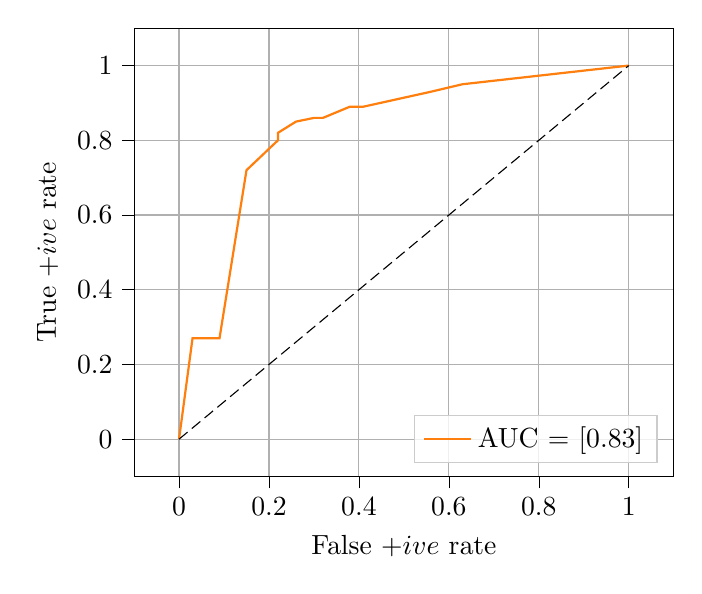
\begin{tikzpicture}
  \begin{axis}
    [
    ylabel={True $+ive$ rate},
    xlabel={False $+ive$ rate},
    tick align=outside,
    tick pos=left,
    ytick style={color=black},
    xtick style={color=black},
    grid style={gridgrey},
    xmajorgrids,
    ymajorgrids,
    legend cell align={left},
    legend columns=1,
    legend style={
      fill opacity=0.8,
      draw opacity=1,
      text opacity=1,
      at={(0.97,0.03)},
      anchor=south east,
      draw=legendgray,
    },
    ]
    \addlegendentry{AUC = $[0.83]$}
    \addplot[thick, darkorange] table {
      0.0 0.0
      0.03 0.27
      0.09 0.27
      0.15 0.72
      0.22 0.8
      0.22 0.82
      0.26 0.85
      0.3 0.86
      0.32 0.86
      0.38 0.89
      0.41 0.89
      0.56 0.93
      0.63 0.95
      1.0 1.0
    };
    \addplot[black, dashed, dash pattern=on 4pt off 2pt] table {
      0 0
      1 1
    };
  \end{axis}
\end{tikzpicture}
}
              \captionsetup{justification=centering}
              \caption{With data leak}
            \end{subfigure}%
            \hspace{0.05\textwidth}
            \begin{subfigure}{0.45\textwidth}
              \centering
              \resizebox{\textwidth}{!}{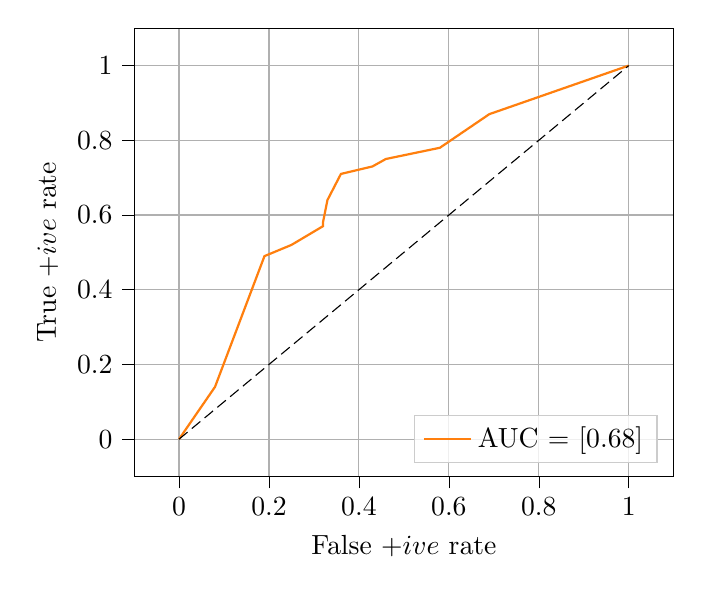
\begin{tikzpicture}
  \begin{axis}
    [
    ylabel={True $+ive$ rate},
    xlabel={False $+ive$ rate},
    tick align=outside,
    tick pos=left,
    ytick style={color=black},
    xtick style={color=black},
    grid style={gridgrey},
    xmajorgrids,
    ymajorgrids,
    legend cell align={left},
    legend columns=1,
    legend style={
      fill opacity=0.8,
      draw opacity=1,
      text opacity=1,
      at={(0.97,0.03)},
      anchor=south east,
      draw=legendgray,
    },
    ]
    \addlegendentry{AUC = $[0.68]$}
    \addplot[thick, darkorange] table {
      0.0 0.0
      0.08 0.14
      0.19 0.49
      0.25 0.52
      0.32 0.57
      0.32 0.58
      0.33 0.64
      0.36 0.71
      0.43 0.73
      0.46 0.75
      0.58 0.78
      0.69 0.87
      1.0 1.0
    };
    \addplot[black, dashed, dash pattern=on 4pt off 2pt] table {
      0 0
      1 1
    };
  \end{axis}
\end{tikzpicture}
}
              \captionsetup{justification=centering}
              \caption{Without data leak}
            \end{subfigure}
            \caption{Porpoise results on \textbf{S\_200} dataset}\label{fig:porpoise_s200}
        \end{figure}

      \paragraph{Mus musculus}
        \noindent
        \begin{table}[H]
            \centering
            \begin{tabular}{lcc}
              \toprule
              \textbf{Metric} & \textbf{Original} & \textbf{Fixed} \\
              \midrule
              Accuracy        & 78\%              & 61\%           \\
              MCC             & 0.44              & 0.23           \\
              Sensitivity     & 78\%              & 66\%           \\
              Specificity     & 78\%              & 57\%           \\
              \bottomrule
            \end{tabular}
            \caption{Results for M\_944 dataset}
            \label{tab:porpoise_pstnpss_mm}
        \end{table}

        \begin{figure}[H]
            \centering
            \begin{subfigure}{0.47\textwidth}
              \centering
              \resizebox{\textwidth}{!}{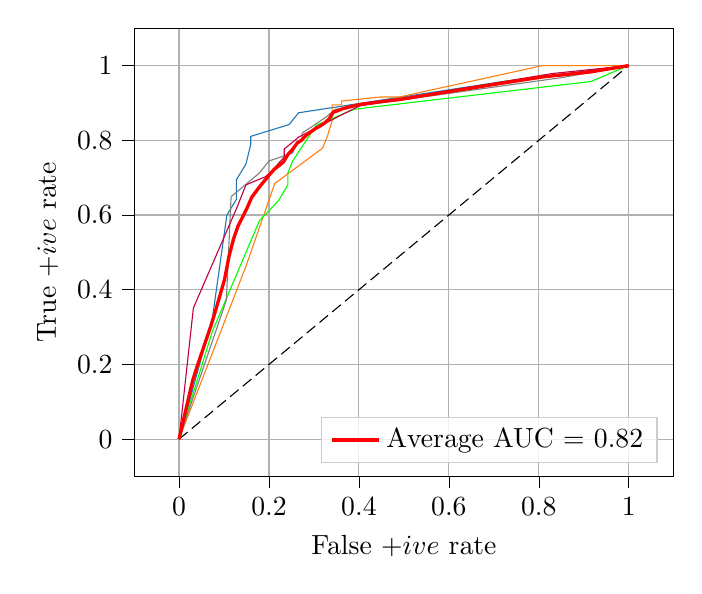
\begin{tikzpicture}
  \begin{axis}
    [
    ylabel={True $+ive$ rate},
    xlabel={False $+ive$ rate},
    tick align=outside,
    tick pos=left,
    ytick style={color=black},
    xtick style={color=black},
    grid style={gridgrey},
    xmajorgrids,
    ymajorgrids,
    legend cell align={left},
    legend columns=1,
    legend style={
      fill opacity=0.8,
      draw opacity=1,
      text opacity=1,
      at={(0.97,0.03)},
      anchor=south east,
      draw=legendgray,
    },
    ]

    \addplot[black, dashed, dash pattern=on 4pt off 2pt, forget plot] table {
      0 0
      1 1
    };


    \addplot[thin, color=steelblue, forget plot] table {
      0.0 0.0
      0.07446808510638298 0.3263157894736842
      0.10638297872340426 0.6
      0.1276595744680851 0.6421052631578947
      0.1276595744680851 0.6947368421052632
      0.14893617021276595 0.7368421052631579
      0.1595744680851064 0.7894736842105263
      0.1595744680851064 0.8105263157894737
      0.24468085106382978 0.8421052631578947
      0.26595744680851063 0.8736842105263158
      0.723404255319149 0.9578947368421052
      1.0 1.0
    };


    \addplot[thin, color=darkorange, forget plot] table {
      0.0 0.0
      0.14893617021276595 0.4631578947368421
      0.2127659574468085 0.6842105263157895
      0.3191489361702128 0.7789473684210526
      0.32978723404255317 0.8105263157894737
      0.3404255319148936 0.8526315789473684
      0.3404255319148936 0.8947368421052632
      0.3617021276595745 0.8947368421052632
      0.3617021276595745 0.9052631578947369
      0.44680851063829785 0.9157894736842105
      0.48936170212765956 0.9157894736842105
      0.8085106382978723 1.0
      1.0 1.0
    };


    \addplot[thin, color=green, forget plot] table {
      0.0 0.0
      0.07368421052631578 0.2872340425531915
      0.17894736842105263 0.5851063829787234
      0.22105263157894736 0.6382978723404256
      0.24210526315789474 0.6808510638297872
      0.24210526315789474 0.7127659574468085
      0.25263157894736843 0.7446808510638298
      0.30526315789473685 0.8404255319148937
      0.3263157894736842 0.851063829787234
      0.3894736842105263 0.8829787234042553
      0.4631578947368421 0.8936170212765957
      0.9157894736842105 0.9574468085106383
      1.0 1.0
    };


    \addplot[thin, color=gray, forget plot] table {
      0.0 0.0
      0.10526315789473684 0.3723404255319149
      0.11578947368421053 0.648936170212766
      0.17894736842105263 0.7127659574468085
      0.2 0.7446808510638298
      0.25263157894736843 0.7659574468085106
      0.2631578947368421 0.7978723404255319
      0.2736842105263158 0.7978723404255319
      0.2736842105263158 0.8191489361702128
      0.3263157894736842 0.8617021276595744
      0.3473684210526316 0.8829787234042553
      0.8526315789473684 0.9680851063829787
      1.0 1.0
    };


    \addplot[thin, color=purple, forget plot] table {
      0.0 0.0
      0.031914893617021274 0.35106382978723405
      0.1276595744680851 0.6170212765957447
      0.14893617021276595 0.6808510638297872
      0.19148936170212766 0.7021276595744681
      0.20212765957446807 0.7127659574468085
      0.23404255319148937 0.7553191489361702
      0.23404255319148937 0.776595744680851
      0.26595744680851063 0.8085106382978723
      0.35106382978723405 0.8617021276595744
      0.40425531914893614 0.8936170212765957
      0.8297872340425532 0.9787234042553191
      1.0 1.0
    };

    \addlegendentry{Average AUC = $0.82$}
    \addplot[very thick, red] table {
      0 0
      0.0 0.0
      0.010101010101010102 0.0523780599144541
      0.020202020202020204 0.1047561198289082
      0.030303030303030304 0.1571341797433623
      0.04040404040404041 0.1955523093858294
      0.05050505050505051 0.2313198193564002
      0.06060606060606061 0.267087329326971
      0.07070707070707072 0.3028548392975418
      0.08080808080808081 0.34241746999492434
      0.09090909090909091 0.3844983024938232
      0.10101010101010102 0.42657913499272215
      0.11111111111111112 0.4890178954083397
      0.12121212121212122 0.5363089111129425
      0.13131313131313133 0.570647960972709
      0.14141414141414144 0.5947472485210448
      0.15151515151515152 0.6192704197631409
      0.16161616161616163 0.6473717578924745
      0.17171717171717174 0.6638861741717286
      0.18181818181818182 0.6797913061182937
      0.19191919191919193 0.6942049272116462
      0.20202020202020204 0.709136493716561
      0.21212121212121213 0.7229376067505966
      0.22222222222222224 0.7320576915100991
      0.23232323232323235 0.7422000030163524
      0.24242424242424243 0.7624863076453222
      0.25252525252525254 0.7757433234924835
      0.26262626262626265 0.7923310145124255
      0.27272727272727276 0.8008780283103963
      0.2828282828282829 0.8137205762934169
      0.29292929292929293 0.8224625440056441
      0.30303030303030304 0.8312045117178715
      0.31313131313131315 0.8378789960860196
      0.32323232323232326 0.8456637319048449
      0.33333333333333337 0.8569347075010635
      0.3434343434343435 0.8756668569862273
      0.3535353535353536 0.8793128047754472
      0.36363636363636365 0.8844110602627753
      0.37373737373737376 0.8876060727942287
      0.38383838383838387 0.8908010853256823
      0.393939393939394 0.8936737251943377
      0.4040404040404041 0.8961395614647001
      0.4141414141414142 0.8978145101356644
      0.42424242424242425 0.899472265597946
      0.43434343434343436 0.9011300210602275
      0.4444444444444445 0.9027877765225092
      0.4545454545454546 0.9042541444249823
      0.4646464646464647 0.9056610331901356
      0.4747474747474748 0.9070621385254579
      0.48484848484848486 0.9084632438607801
      0.494949494949495 0.9101592278067707
      0.5050505050505051 0.9120933829383008
      0.5151515151515152 0.9140275380698307
      0.5252525252525253 0.9159616932013609
      0.5353535353535354 0.917895848332891
      0.5454545454545455 0.9198300034644211
      0.5555555555555556 0.9217641585959511
      0.5656565656565657 0.9236983137274812
      0.5757575757575758 0.9256324688590112
      0.5858585858585859 0.9275666239905412
      0.595959595959596 0.9295007791220714
      0.6060606060606061 0.9314349342536014
      0.6161616161616162 0.9333690893851315
      0.6262626262626263 0.9353032445166616
      0.6363636363636365 0.9372373996481917
      0.6464646464646465 0.9391715547797217
      0.6565656565656566 0.9411057099112519
      0.6666666666666667 0.9430398650427818
      0.6767676767676768 0.9449740201743119
      0.686868686868687 0.9469081753058418
      0.696969696969697 0.9488423304373719
      0.7070707070707072 0.950776485568902
      0.7171717171717172 0.9527106407004322
      0.7272727272727273 0.954620144840359
      0.7373737373737375 0.9564899334938136
      0.7474747474747475 0.9583597221472686
      0.7575757575757577 0.9602295108007237
      0.7676767676767677 0.9620992994541785
      0.7777777777777778 0.9639690881076334
      0.787878787878788 0.9658388767610881
      0.797979797979798 0.967708665414543
      0.8080808080808082 0.969578454067998
      0.8181818181818182 0.9709378758952966
      0.8282828282828284 0.972274614752544
      0.8383838383838385 0.9734824045446718
      0.8484848484848485 0.9746676282504039
      0.8585858585858587 0.9759101626517446
      0.8686868686868687 0.9771926098589553
      0.8787878787878789 0.9784750570661661
      0.888888888888889 0.979757504273377
      0.8989898989898991 0.981039951480588
      0.9090909090909092 0.9823223986877988
      0.9191919191919192 0.9838527479736886
      0.9292929292929294 0.9858711544769776
      0.9393939393939394 0.9878895609802665
      0.9494949494949496 0.9899079674835554
      0.9595959595959597 0.9919263739868445
      0.9696969696969697 0.9939447804901332
      0.9797979797979799 0.9959631869934222
      0.98989898989899 0.997981593496711
      1.0 1.0
    };


  \end{axis}
\end{tikzpicture}
}
              \captionsetup{justification=centering}
              \caption{With data leak}
            \end{subfigure}%
            \hspace{0.05\textwidth}
            \begin{subfigure}{0.47\textwidth}
              \centering
              \resizebox{\textwidth}{!}{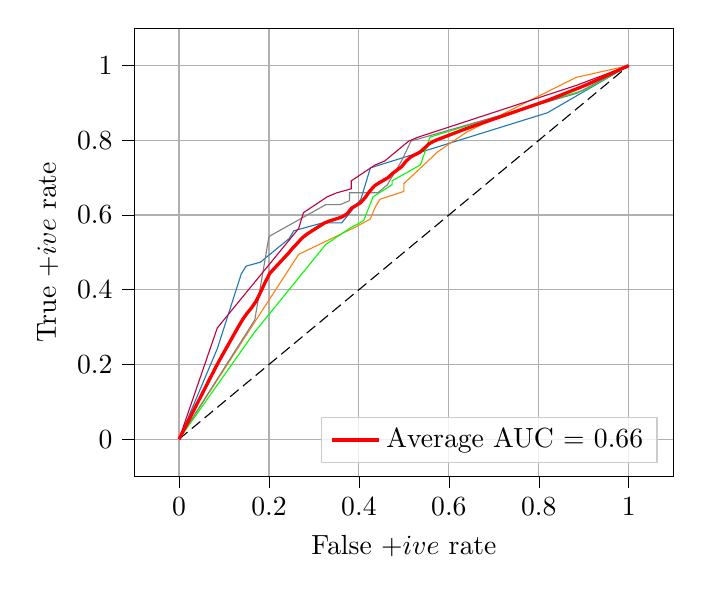
\begin{tikzpicture}
  \begin{axis}
    [
    ylabel={True $+ive$ rate},
    xlabel={False $+ive$ rate},
    tick align=outside,
    tick pos=left,
    ytick style={color=black},
    xtick style={color=black},
    grid style={gridgrey},
    xmajorgrids,
    ymajorgrids,
    legend cell align={left},
    legend columns=1,
    legend style={
      fill opacity=0.8,
      draw opacity=1,
      text opacity=1,
      at={(0.97,0.03)},
      anchor=south east,
      draw=legendgray,
    },
    ]

    \addplot[black, dashed, dash pattern=on 4pt off 2pt, forget plot] table {
      0 0
      1 1
    };


    \addplot[thin, color=steelblue, forget plot] table {
      0.0 0.0
      0.0851063829787234 0.24210526315789474
      0.13829787234042554 0.4421052631578947
      0.14893617021276595 0.4631578947368421
      0.18085106382978725 0.47368421052631576
      0.24468085106382978 0.5368421052631579
      0.2553191489361702 0.5578947368421052
      0.3191489361702128 0.5789473684210527
      0.3617021276595745 0.5789473684210527
      0.40425531914893614 0.6421052631578947
      0.425531914893617 0.7263157894736842
      0.8191489361702128 0.8736842105263158
      1.0 1.0
    };


    \addplot[thin, color=darkorange, forget plot] table {
      0.0 0.0
      0.18085106382978725 0.3368421052631579
      0.26595744680851063 0.49473684210526314
      0.39361702127659576 0.5684210526315789
      0.425531914893617 0.5894736842105263
      0.43617021276595747 0.6210526315789474
      0.44680851063829785 0.6421052631578947
      0.5 0.6631578947368421
      0.5 0.6842105263157895
      0.574468085106383 0.7684210526315789
      0.6382978723404256 0.8210526315789474
      0.8829787234042553 0.968421052631579
      1.0 1.0
    };


    \addplot[thin, color=green, forget plot] table {
      0.0 0.0
      0.16842105263157894 0.2872340425531915
      0.3263157894736842 0.5212765957446809
      0.37894736842105264 0.5638297872340425
      0.4105263157894737 0.5851063829787234
      0.43157894736842106 0.648936170212766
      0.47368421052631576 0.6808510638297872
      0.47368421052631576 0.6914893617021277
      0.5368421052631579 0.7340425531914894
      0.5578947368421052 0.8085106382978723
      0.9052631578947369 0.9361702127659575
      1.0 1.0
    };


    \addplot[thin, color=gray, forget plot] table {
      0.0 0.0
      0.16842105263157894 0.3191489361702128
      0.2 0.5425531914893617
      0.3263157894736842 0.6276595744680851
      0.35789473684210527 0.6276595744680851
      0.37894736842105264 0.6382978723404256
      0.37894736842105264 0.6595744680851063
      0.4421052631578947 0.6595744680851063
      0.4631578947368421 0.6808510638297872
      0.49473684210526314 0.7446808510638298
      0.5157894736842106 0.7978723404255319
      0.8842105263157894 0.925531914893617
      1.0 1.0
    };


    \addplot[thin, color=purple, forget plot] table {
      0.0 0.0
      0.0851063829787234 0.2978723404255319
      0.26595744680851063 0.5638297872340425
      0.2765957446808511 0.6063829787234043
      0.32978723404255317 0.648936170212766
      0.35106382978723405 0.6595744680851063
      0.3829787234042553 0.6702127659574468
      0.3829787234042553 0.6914893617021277
      0.43617021276595747 0.7340425531914894
      0.4574468085106383 0.7446808510638298
      0.5106382978723404 0.7978723404255319
      0.5319148936170213 0.8085106382978723
      0.8829787234042553 0.9468085106382979
      1.0 1.0
    };

    \addlegendentry{Average AUC = $0.66$}
    \addplot[very thick, red] table {
      0 0
      0.0 0.0
      0.010101010101010102 0.023853887834274504
      0.020202020202020204 0.04770777566854901
      0.030303030303030304 0.07156166350282352
      0.04040404040404041 0.09541555133709802
      0.05050505050505051 0.11926943917137253
      0.06060606060606061 0.14312332700564703
      0.07070707070707072 0.16697721483992153
      0.08080808080808081 0.19083110267419603
      0.09090909090909091 0.2133919747172003
      0.10101010101010102 0.2349950572851897
      0.11111111111111112 0.25659813985317903
      0.12121212121212122 0.2782012224211684
      0.13131313131313133 0.2998043049891578
      0.14141414141414144 0.3202973397102572
      0.15151515151515152 0.3374517247769175
      0.16161616161616163 0.35212515999420685
      0.17171717171717174 0.3700659316969178
      0.18181818181818182 0.3948783567178271
      0.19191919191919193 0.42088252371995216
      0.20202020202020204 0.44430054558274046
      0.21212121212121213 0.4573739868881823
      0.22222222222222224 0.47044742819362406
      0.23232323232323235 0.4835208694990659
      0.24242424242424243 0.4965943108045078
      0.25252525252525254 0.5112201178728417
      0.26262626262626265 0.523882430346102
      0.27272727272727276 0.537317520105874
      0.2828282828282829 0.5475974753130408
      0.29292929292929293 0.5554016084699176
      0.30303030303030304 0.5632057416267943
      0.31313131313131315 0.571009874783671
      0.32323232323232326 0.5785446476711874
      0.33333333333333337 0.5835784496702751
      0.3434343434343435 0.5873879519344245
      0.3535353535353536 0.5911150700736367
      0.36363636363636365 0.5957423054735485
      0.37373737373737376 0.6032343592701936
      0.38383838383838387 0.6186911669890394
      0.393939393939394 0.6258382254798829
      0.4040404040404041 0.6331465457109354
      0.4141414141414142 0.6470508745536743
      0.42424242424242425 0.6641204881966359
      0.43434343434343436 0.6776863914713859
      0.4444444444444445 0.685925920321217
      0.4545454545454546 0.6928134521572372
      0.4646464646464647 0.699973292747089
      0.4747474747474748 0.7112738310946598
      0.48484848484848486 0.7202944783325522
      0.494949494949495 0.7293366170812978
      0.5050505050505051 0.744331099616654
      0.5151515151515152 0.7554061963244496
      0.5252525252525253 0.7617964506878281
      0.5353535353535354 0.7678356026111295
      0.5454545454545455 0.7786657333099358
      0.5555555555555556 0.7903483606059194
      0.5656565656565657 0.7971104088033742
      0.5757575757575758 0.8023105574098143
      0.5858585858585859 0.8069709728449421
      0.595959595959596 0.81163138828007
      0.6060606060606061 0.8162918037151977
      0.6161616161616162 0.8209522191503258
      0.6262626262626263 0.8256126345854534
      0.6363636363636365 0.8302730500205813
      0.6464646464646465 0.8345704146578757
      0.6565656565656566 0.8387817935798939
      0.6666666666666667 0.842993172501912
      0.6767676767676768 0.8472045514239301
      0.686868686868687 0.8514159303459483
      0.696969696969697 0.8556273092679663
      0.7070707070707072 0.8598386881899845
      0.7171717171717172 0.8640500671120026
      0.7272727272727273 0.8682614460340206
      0.7373737373737375 0.8724728249560387
      0.7474747474747475 0.8766842038780569
      0.7575757575757577 0.880895582800075
      0.7676767676767677 0.8851069617220929
      0.7777777777777778 0.8893183406441112
      0.787878787878788 0.8935297195661291
      0.797979797979798 0.8977410984881473
      0.8080808080808082 0.9019524774101656
      0.8181818181818182 0.9061638563321835
      0.8282828282828284 0.9109672147935497
      0.8383838383838385 0.9158332534414348
      0.8484848484848485 0.9206992920893201
      0.8585858585858587 0.9255653307372054
      0.8686868686868687 0.9304313693850906
      0.8787878787878789 0.935297408032976
      0.888888888888889 0.9401196870889251
      0.8989898989898991 0.945035832996262
      0.9090909090909092 0.9501864317492705
      0.9191919191919192 0.9557212726660183
      0.9292929292929294 0.961256113582766
      0.9393939393939394 0.9667909544995137
      0.9494949494949496 0.9723257954162614
      0.9595959595959597 0.9778606363330091
      0.9696969696969697 0.9833954772497568
      0.9797979797979799 0.9889303181665046
      0.98989898989899 0.9944651590832523
      1.0 1.0
    };


  \end{axis}
\end{tikzpicture}
}
              \captionsetup{justification=centering}
              \caption{Without data leak}
            \end{subfigure}
            \caption{Porpoise results on \textbf{H\_944} dataset}\label{fig:porpoise_m944}
        \end{figure}

    \subsubsection{PseU-ST}
      This study~\cite{zhang_pseu-st_2023} takes a similar approach as Porpoise~\cite{li_porpoise_2021} however it takes different encoding schemes and different models, but the mistake is somewhat similar, firstly it is dependent on PSTNPss and we can see the different in performance, another mistake is the use of Best feature selection.
      Firstly the encoding is applied on the whole training set and feature selection is also done on the whole dataset instead of performing best feature selection on each k-fold.
      As mentioned in the earlier section, applying position specific propensity on the whole train dataset before k-fold adds label information which leads to unreliable results and performing feature selection on the whole dataset instead of each k-fold will also add some bias in the predictions

      \paragraph{Homo sapiens}
        \noindent
        \begin{table}[H]
            \centering
            \begin{minipage}{0.45\textwidth}
              \centering
              \begin{tabular}{lcc}
                \toprule
                \textbf{Metric} & \textbf{Original} & \textbf{Fixed} \\
                \midrule
                Accuracy        & 93\%              & 59\%           \\
                MCC             & 0.87              & 0.18           \\
                Sensitivity     & 94\%              & 58\%           \\
                Specificity     & 93\%              & 61\%           \\
                \bottomrule
              \end{tabular}
              \caption{Results for H\_990 dataset}
            \end{minipage}%
            \hfill
            \begin{minipage}{0.45\textwidth}
              \centering
              \begin{tabular}{lcc}
                \toprule
                \textbf{Metric} & \textbf{Original} & \textbf{Fixed} \\
                \midrule
                Accuracy        & 89\%              & 64\%           \\
                MCC             & 0.79              & 0.28           \\
                Sensitivity     & 98\%              & 65\%           \\
                Specificity     & 81\%              & 63\%           \\
                \bottomrule
              \end{tabular}
              \caption{Results for H\_200 dataset}
            \end{minipage}\label{tab:pseust_pstnpss_hs}
        \end{table}

        \begin{figure}[H]
            \centering
            \begin{subfigure}{0.47\textwidth}
              \centering
              \resizebox{\textwidth}{!}{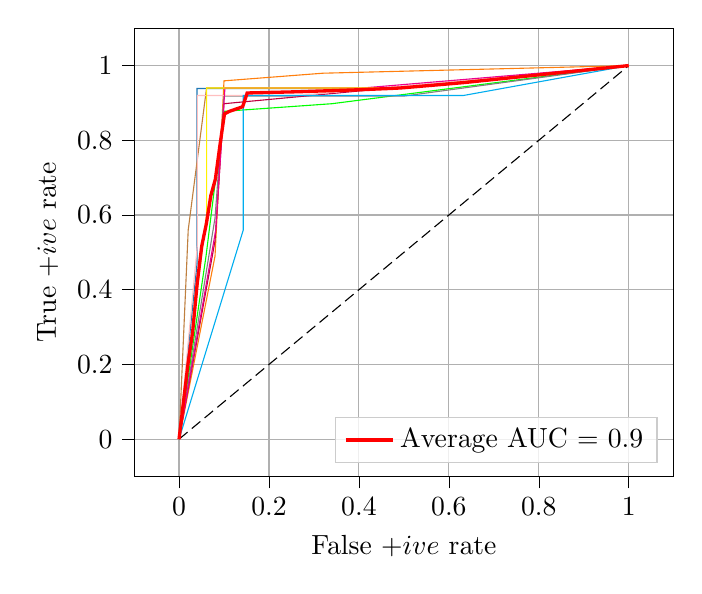
\begin{tikzpicture}
  \begin{axis}
    [
    ylabel={True $+ive$ rate},
    xlabel={False $+ive$ rate},
    tick align=outside,
    tick pos=left,
    ytick style={color=black},
    xtick style={color=black},
    grid style={gridgrey},
    xmajorgrids,
    ymajorgrids,
    legend cell align={left},
    legend columns=1,
    legend style={
      fill opacity=0.8,
      draw opacity=1,
      text opacity=1,
      at={(0.97,0.03)},
      anchor=south east,
      draw=legendgray,
    },
    ]

    \addplot[black, dashed, dash pattern=on 4pt off 2pt, forget plot] table {
      0 0
      1 1
    };


    \addplot[thin, color=steelblue, forget plot] table {
      0.0 0.0
      0.04 0.46938775510204084
      0.04 0.9387755102040817
      0.48 0.9387755102040817
      1.0 1.0
    };


    \addplot[thin, color=darkorange, forget plot] table {
      0.0 0.0
      0.08 0.4897959183673469
      0.1 0.9591836734693877
      0.32 0.9795918367346939
      1.0 1.0
    };


    \addplot[thin, color=green, forget plot] table {
      0.0 0.0
      0.06 0.4897959183673469
      0.1 0.8775510204081632
      0.34 0.8979591836734694
      1.0 1.0
    };


    \addplot[thin, color=gray, forget plot] table {
      0.0 0.0
      0.08 0.5918367346938775
      0.1 0.9183673469387755
      0.5 0.9183673469387755
      1.0 1.0
    };


    \addplot[thin, color=purple, forget plot] table {
      0.0 0.0
      0.08 0.5306122448979592
      0.1 0.8979591836734694
      0.46 0.9387755102040817
      1.0 1.0
    };


    \addplot[thin, color=brown, forget plot] table {
      0.0 0.0
      0.02040816326530612 0.56
      0.061224489795918366 0.94
      0.4897959183673469 0.94
      1.0 1.0
    };


    \addplot[thin, color=pink, forget plot] table {
      0.0 0.0
      0.04081632653061224 0.52
      0.04081632653061224 0.92
      0.2653061224489796 0.92
      1.0 1.0
    };


    \addplot[thin, color=cyan, forget plot] table {
      0.0 0.0
      0.14285714285714285 0.56
      0.14285714285714285 0.92
      0.6326530612244898 0.92
      1.0 1.0
    };


    \addplot[thin, color=magenta, forget plot] table {
      0.0 0.0
      0.08163265306122448 0.56
      0.10204081632653061 0.94
      0.40816326530612246 0.94
      1.0 1.0
    };


    \addplot[thin, color=yellow, forget plot] table {
      0.0 0.0
      0.061224489795918366 0.6
      0.061224489795918366 0.94
      0.4897959183673469 0.94
      1.0 1.0
    };

    \addlegendentry{Average AUC = $0.9$}
    \addplot[very thick, red] table {
      0 0
      0.0 0.0
      0.010101010101010102 0.10182931354359928
      0.020202020202020204 0.20365862708719856
      0.030303030303030304 0.28754854669140384
      0.04040404040404041 0.41752937538651824
      0.05050505050505051 0.5168488971346115
      0.06060606060606061 0.5757359307359307
      0.07070707070707072 0.6519550608122039
      0.08080808080808081 0.6960639043496186
      0.09090909090909091 0.7864044526901669
      0.10101010101010102 0.870889852972104
      0.11111111111111112 0.877062759110378
      0.12121212121212122 0.8813164733294604
      0.13131313131313133 0.8855701875485424
      0.14141414141414144 0.8898239017676246
      0.15151515151515152 0.9266836765927673
      0.16161616161616163 0.9269777948522536
      0.17171717171717174 0.9272719131117398
      0.18181818181818182 0.927566031371226
      0.19191919191919193 0.9278601496307124
      0.20202020202020204 0.9281542678901985
      0.21212121212121213 0.9284483861496847
      0.22222222222222224 0.9287425044091708
      0.23232323232323235 0.9290366226686573
      0.24242424242424243 0.9293307409281434
      0.25252525252525254 0.9296248591876296
      0.26262626262626265 0.9299189774471159
      0.27272727272727276 0.9302939037874103
      0.2828282828282829 0.930698010823552
      0.29292929292929293 0.9311021178596934
      0.30303030303030304 0.9315062248958352
      0.31313131313131315 0.9319103319319769
      0.32323232323232326 0.9322941553725865
      0.33333333333333337 0.9326348761726913
      0.3434343434343435 0.9329994908278584
      0.3535353535353536 0.933410487672265
      0.36363636363636365 0.9338214845166716
      0.37373737373737376 0.9342324813610782
      0.38383838383838387 0.9346434782054847
      0.393939393939394 0.9350544750498914
      0.4040404040404041 0.9354654718942979
      0.4141414141414142 0.9359370747993104
      0.42424242424242425 0.9364504749874998
      0.43434343434343436 0.936963875175689
      0.4444444444444445 0.9374772753638781
      0.4545454545454546 0.9379906755520674
      0.4646464646464647 0.9385040757402565
      0.4747474747474748 0.939017475928446
      0.48484848484848486 0.9395879618880066
      0.494949494949495 0.9403415028877653
      0.5050505050505051 0.9412938647492017
      0.5151515151515152 0.9423286838359528
      0.5252525252525253 0.9433635029227038
      0.5353535353535354 0.9443983220094548
      0.5454545454545455 0.9454331410962057
      0.5555555555555556 0.9464679601829568
      0.5656565656565657 0.9475027792697077
      0.5757575757575758 0.9485375983564589
      0.5858585858585859 0.9495724174432099
      0.595959595959596 0.9506072365299609
      0.6060606060606061 0.9516420556167118
      0.6161616161616162 0.9526768747034626
      0.6262626262626263 0.9537116937902136
      0.6363636363636365 0.9548273209577729
      0.6464646464646465 0.9560821175978347
      0.6565656565656566 0.9573369142378965
      0.6666666666666667 0.9585917108779585
      0.6767676767676768 0.9598465075180203
      0.686868686868687 0.9611013041580823
      0.696969696969697 0.9623561007981438
      0.7070707070707072 0.9636108974382059
      0.7171717171717172 0.9648656940782676
      0.7272727272727273 0.9661204907183297
      0.7373737373737375 0.9673752873583915
      0.7474747474747475 0.9686300839984534
      0.7575757575757577 0.9698848806385151
      0.7676767676767677 0.971139677278577
      0.7777777777777778 0.972394473918639
      0.787878787878788 0.9736492705587008
      0.797979797979798 0.9749040671987625
      0.8080808080808082 0.9761588638388246
      0.8181818181818182 0.9774136604788864
      0.8282828282828284 0.9786684571189482
      0.8383838383838385 0.9799232537590102
      0.8484848484848485 0.981178050399072
      0.8585858585858587 0.9824328470391339
      0.8686868686868687 0.9836876436791957
      0.8787878787878789 0.9849424403192575
      0.888888888888889 0.9861972369593193
      0.8989898989898991 0.9874520335993815
      0.9090909090909092 0.9887068302394431
      0.9191919191919192 0.9899616268795048
      0.9292929292929294 0.9912164235195668
      0.9393939393939394 0.9924712201596287
      0.9494949494949496 0.9937260167996905
      0.9595959595959597 0.9949808134397525
      0.9696969696969697 0.9962356100798143
      0.9797979797979799 0.9974904067198762
      0.98989898989899 0.9987452033599382
      1.0 1.0
    };


  \end{axis}
\end{tikzpicture}
}
              \captionsetup{justification=centering}
              \caption{With data leak}
            \end{subfigure}%
            \hspace{0.05\textwidth}
            \begin{subfigure}{0.47\textwidth}
              \centering
              \resizebox{\textwidth}{!}{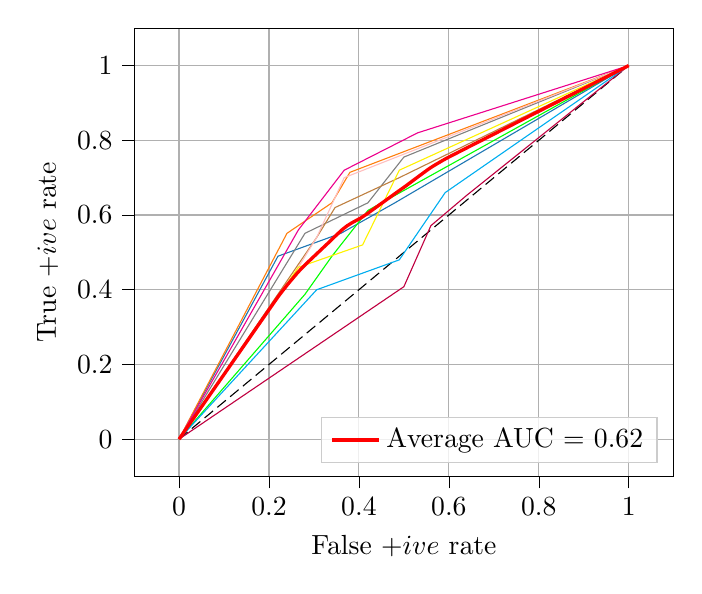
\begin{tikzpicture}
  \begin{axis}
    [
    ylabel={True $+ive$ rate},
    xlabel={False $+ive$ rate},
    tick align=outside,
    tick pos=left,
    ytick style={color=black},
    xtick style={color=black},
    grid style={gridgrey},
    xmajorgrids,
    ymajorgrids,
    legend cell align={left},
    legend columns=1,
    legend style={
      fill opacity=0.8,
      draw opacity=1,
      text opacity=1,
      at={(0.97,0.03)},
      anchor=south east,
      draw=legendgray,
    },
    ]

    \addplot[black, dashed, dash pattern=on 4pt off 2pt, forget plot] table {
      0 0
      1 1
    };


    \addplot[thin, color=steelblue, forget plot] table {
      0.0 0.0
      0.22 0.4897959183673469
      0.36 0.5510204081632653
      0.48 0.6326530612244898
      1.0 1.0
    };


    \addplot[thin, color=darkorange, forget plot] table {
      0.0 0.0
      0.24 0.5510204081632653
      0.34 0.6326530612244898
      0.38 0.7142857142857143
      1.0 1.0
    };


    \addplot[thin, color=green, forget plot] table {
      0.0 0.0
      0.28 0.3877551020408163
      0.34 0.4897959183673469
      0.42 0.6122448979591837
      1.0 1.0
    };


    \addplot[thin, color=gray, forget plot] table {
      0.0 0.0
      0.28 0.5510204081632653
      0.42 0.6326530612244898
      0.5 0.7551020408163265
      1.0 1.0
    };


    \addplot[thin, color=purple, forget plot] table {
      0.0 0.0
      0.5 0.40816326530612246
      0.56 0.5714285714285714
      0.64 0.6530612244897959
      1.0 1.0
    };


    \addplot[thin, color=brown, forget plot] table {
      0.0 0.0
      0.30612244897959184 0.54
      0.3469387755102041 0.62
      0.4897959183673469 0.7
      1.0 1.0
    };


    \addplot[thin, color=pink, forget plot] table {
      0.0 0.0
      0.24489795918367346 0.42
      0.30612244897959184 0.54
      0.3673469387755102 0.7
      1.0 1.0
    };


    \addplot[thin, color=cyan, forget plot] table {
      0.0 0.0
      0.30612244897959184 0.4
      0.4897959183673469 0.48
      0.5918367346938775 0.66
      1.0 1.0
    };


    \addplot[thin, color=magenta, forget plot] table {
      0.0 0.0
      0.2653061224489796 0.56
      0.3673469387755102 0.72
      0.5306122448979592 0.82
      1.0 1.0
    };


    \addplot[thin, color=yellow, forget plot] table {
      0.0 0.0
      0.2653061224489796 0.46
      0.40816326530612246 0.52
      0.4897959183673469 0.72
      1.0 1.0
    };

    \addlegendentry{Average AUC = $0.62$}
    \addplot[very thick, red] table {
      0 0
      0.0 0.0
      0.010101010101010102 0.017496607789928755
      0.020202020202020204 0.03499321557985751
      0.030303030303030304 0.05248982336978626
      0.04040404040404041 0.06998643115971502
      0.05050505050505051 0.08748303894964378
      0.06060606060606061 0.10497964673957252
      0.07070707070707072 0.12247625452950128
      0.08080808080808081 0.13997286231943004
      0.09090909090909091 0.1574694701093588
      0.10101010101010102 0.17496607789928756
      0.11111111111111112 0.1924626856892163
      0.12121212121212122 0.20995929347914505
      0.13131313131313133 0.22745590126907378
      0.14141414141414144 0.24495250905900257
      0.15151515151515152 0.2624491168489313
      0.16161616161616163 0.2799457246388601
      0.17171717171717174 0.2974423324287888
      0.18181818181818182 0.3149389402187176
      0.19191919191919193 0.33243554800864633
      0.20202020202020204 0.3499321557985751
      0.21212121212121213 0.3674287635885038
      0.22222222222222224 0.3845278097563812
      0.23232323232323235 0.4002173192642581
      0.24242424242424243 0.41554813984201744
      0.25252525252525254 0.42992998082793993
      0.26262626262626265 0.44437242787446873
      0.27272727272727276 0.45743705274317514
      0.2828282828282829 0.46970178755484876
      0.29292929292929293 0.48118906852784404
      0.30303030303030304 0.4926763495008393
      0.31313131313131315 0.5041483667252376
      0.32323232323232326 0.5156136499429017
      0.33333333333333337 0.5270789331605659
      0.3434343434343435 0.5389063410260689
      0.3535353535353536 0.5505131758138562
      0.36363636363636365 0.5617177371381452
      0.37373737373737376 0.5711017504163763
      0.38383838383838387 0.5787310147569091
      0.393939393939394 0.5853707923936693
      0.4040404040404041 0.5920105700304297
      0.4141414141414142 0.5998639118807542
      0.42424242424242425 0.6085904473136318
      0.43434343434343436 0.6173670460618789
      0.4444444444444445 0.6261436448101261
      0.4545454545454546 0.6349202435583733
      0.4646464646464647 0.6436968423066204
      0.4747474747474748 0.6524734410548676
      0.48484848484848486 0.6612627255300861
      0.494949494949495 0.6697850089287798
      0.5050505050505051 0.6784741142885812
      0.5151515151515152 0.6875995557990044
      0.5252525252525253 0.6967249973094275
      0.5353535353535354 0.705741852961265
      0.5454545454545455 0.7146359593816575
      0.5555555555555556 0.72353006580205
      0.5656565656565657 0.7314621712604414
      0.5757575757575758 0.738638418820118
      0.5858585858585859 0.7458146663797944
      0.595959595959596 0.7526070755556327
      0.6060606060606061 0.7588429190749052
      0.6161616161616162 0.7650787625941777
      0.6262626262626263 0.7713146061134499
      0.6363636363636365 0.7775504496327226
      0.6464646464646465 0.7837496454962997
      0.6565656565656566 0.789928227053548
      0.6666666666666667 0.7961068086107967
      0.6767676767676768 0.8022853901680455
      0.686868686868687 0.8084639717252939
      0.696969696969697 0.8146425532825425
      0.7070707070707072 0.8208211348397911
      0.7171717171717172 0.8269997163970398
      0.7272727272727273 0.8331782979542881
      0.7373737373737375 0.8393568795115369
      0.7474747474747475 0.8455354610687854
      0.7575757575757577 0.851714042626034
      0.7676767676767677 0.8578926241832827
      0.7777777777777778 0.8640712057405311
      0.787878787878788 0.8702497872977798
      0.797979797979798 0.8764283688550283
      0.8080808080808082 0.8826069504122771
      0.8181818181818182 0.8887855319695255
      0.8282828282828284 0.8949641135267742
      0.8383838383838385 0.9011426950840227
      0.8484848484848485 0.9073212766412713
      0.8585858585858587 0.9134998581985198
      0.8686868686868687 0.9196784397557684
      0.8787878787878789 0.9258570213130171
      0.888888888888889 0.9320356028702657
      0.8989898989898991 0.9382141844275141
      0.9090909090909092 0.9443927659847627
      0.9191919191919192 0.9505713475420112
      0.9292929292929294 0.95674992909926
      0.9393939393939394 0.9629285106565085
      0.9494949494949496 0.9691070922137573
      0.9595959595959597 0.9752856737710056
      0.9696969696969697 0.9814642553282542
      0.9797979797979799 0.9876428368855029
      0.98989898989899 0.9938214184427515
      1.0 1.0
    };


  \end{axis}
\end{tikzpicture}
}
              \captionsetup{justification=centering}
              \caption{Without data leak}
            \end{subfigure}
            \caption{PseU-ST results on \textbf{H\_990} dataset}\label{fig:pseu-st_h990}
        \end{figure}

        \begin{figure}[H]
            \centering
            \begin{subfigure}{0.45\textwidth}
              \centering
              \resizebox{\textwidth}{!}{\input{images/tikz/pseu-st_dl_h_200}}
              \captionsetup{justification=centering}
              \caption{With data leak}
            \end{subfigure}%
            \hspace{0.05\textwidth}
            \begin{subfigure}{0.45\textwidth}
              \centering
              \resizebox{\textwidth}{!}{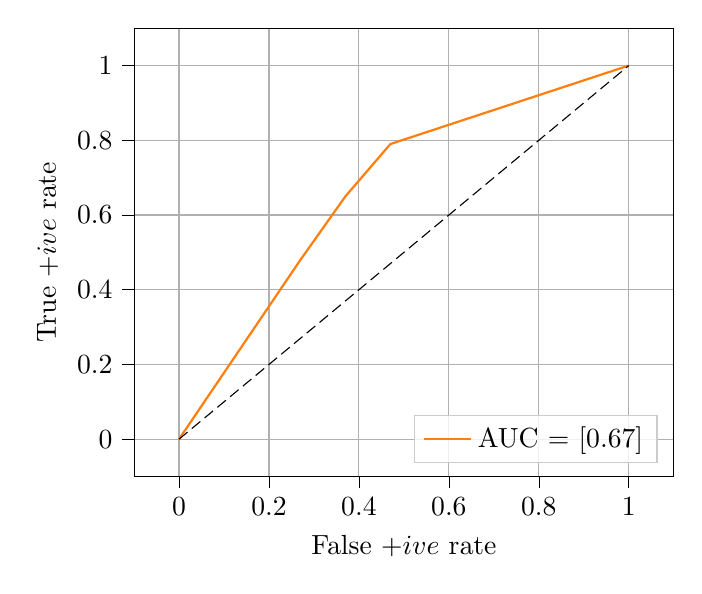
\begin{tikzpicture}
  \begin{axis}
    [
    ylabel={True $+ive$ rate},
    xlabel={False $+ive$ rate},
    tick align=outside,
    tick pos=left,
    ytick style={color=black},
    xtick style={color=black},
    grid style={gridgrey},
    xmajorgrids,
    ymajorgrids,
    legend cell align={left},
    legend columns=1,
    legend style={
      fill opacity=0.8,
      draw opacity=1,
      text opacity=1,
      at={(0.97,0.03)},
      anchor=south east,
      draw=legendgray,
    },
    ]
    \addlegendentry{AUC = $[0.67]$}
    \addplot[thick, darkorange] table {
      0.0 0.0
      0.27 0.48
      0.37 0.65
      0.47 0.79
      1.0 1.0
    };
    \addplot[black, dashed, dash pattern=on 4pt off 2pt] table {
      0 0
      1 1
    };
  \end{axis}
\end{tikzpicture}
}
              \captionsetup{justification=centering}
              \caption{Without data leak}
            \end{subfigure}
            \caption{PseU-ST results on \textbf{H\_200} dataset}\label{fig:pseu-st_h200}
        \end{figure}

      \paragraph{Saccharomyces cerevisiae}
        \noindent
        \begin{table}[H]
            \centering
            \begin{minipage}{0.45\textwidth}
              \centering
              \begin{tabular}{lcc}
                \toprule
                \textbf{Metric} & \textbf{Original} & \textbf{Fixed} \\
                \midrule
                Accuracy        & 88\%              & 65\%           \\
                MCC             & 0.75              & 0.31           \\
                Sensitivity     & 87\%              & 65\%           \\
                Specificity     & 89\%              & 66\%           \\
                \bottomrule
              \end{tabular}
              \caption{Results for S\_628 dataset}
            \end{minipage}%
            \hfill
            \begin{minipage}{0.45\textwidth}
              \centering
              \begin{tabular}{lcc}
                \toprule
                \textbf{Metric} & \textbf{Original} & \textbf{Fixed} \\
                \midrule
                Accuracy        & 83\%              & 69\%           \\
                MCC             & 0.67              & 0.39           \\
                Sensitivity     & 83\%              & 70\%           \\
                Specificity     & 84\%              & 69\%           \\
                \bottomrule
              \end{tabular}
              \caption{Results for S\_200 dataset}
            \end{minipage}\label{tab:pseu-st_pstnpss_sc}
        \end{table}

        \begin{figure}[H]
            \centering
            \begin{subfigure}{0.47\textwidth}
              \centering
              \resizebox{\textwidth}{!}{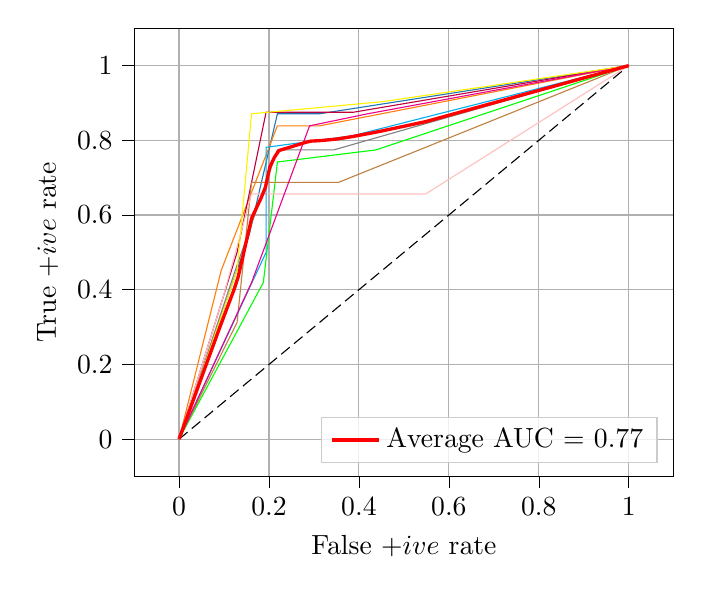
\begin{tikzpicture}
  \begin{axis}
    [
    ylabel={True $+ive$ rate},
    xlabel={False $+ive$ rate},
    tick align=outside,
    tick pos=left,
    ytick style={color=black},
    xtick style={color=black},
    grid style={gridgrey},
    xmajorgrids,
    ymajorgrids,
    legend cell align={left},
    legend columns=1,
    legend style={
      fill opacity=0.8,
      draw opacity=1,
      text opacity=1,
      at={(0.97,0.03)},
      anchor=south east,
      draw=legendgray,
    },
    ]

    \addplot[black, dashed, dash pattern=on 4pt off 2pt, forget plot] table {
      0 0
      1 1
    };


    \addplot[thin, color=steelblue, forget plot] table {
      0.0 0.0
      0.15625 0.5483870967741935
      0.21875 0.8709677419354839
      0.3125 0.8709677419354839
      1.0 1.0
    };


    \addplot[thin, color=darkorange, forget plot] table {
      0.0 0.0
      0.09375 0.45161290322580644
      0.21875 0.8387096774193549
      0.3125 0.8387096774193549
      1.0 1.0
    };


    \addplot[thin, color=green, forget plot] table {
      0.0 0.0
      0.1875 0.41935483870967744
      0.21875 0.7419354838709677
      0.4375 0.7741935483870968
      1.0 1.0
    };


    \addplot[thin, color=gray, forget plot] table {
      0.0 0.0
      0.125 0.45161290322580644
      0.21875 0.7741935483870968
      0.34375 0.7741935483870968
      1.0 1.0
    };


    \addplot[thin, color=purple, forget plot] table {
      0.0 0.0
      0.12903225806451613 0.5
      0.1935483870967742 0.875
      0.3870967741935484 0.875
      1.0 1.0
    };


    \addplot[thin, color=brown, forget plot] table {
      0.0 0.0
      0.12903225806451613 0.3125
      0.16129032258064516 0.6875
      0.3548387096774194 0.6875
      1.0 1.0
    };


    \addplot[thin, color=pink, forget plot] table {
      0.0 0.0
      0.0967741935483871 0.375
      0.16129032258064516 0.65625
      0.5483870967741935 0.65625
      1.0 1.0
    };


    \addplot[thin, color=cyan, forget plot] table {
      0.0 0.0
      0.1935483870967742 0.5
      0.1935483870967742 0.78125
      0.3870967741935484 0.8125
      1.0 1.0
    };


    \addplot[thin, color=magenta, forget plot] table {
      0.0 0.0
      0.16129032258064516 0.41935483870967744
      0.2903225806451613 0.8387096774193549
      0.41935483870967744 0.8709677419354839
      1.0 1.0
    };


    \addplot[thin, color=yellow, forget plot] table {
      0.0 0.0
      0.12903225806451613 0.45161290322580644
      0.16129032258064516 0.8709677419354839
      0.45161290322580644 0.9032258064516129
      1.0 1.0
    };

    \addlegendentry{Average AUC = $0.77$}
    \addplot[very thick, red] table {
      0 0
      0.0 0.0
      0.010101010101010102 0.03336520446399479
      0.020202020202020204 0.06673040892798958
      0.030303030303030304 0.10009561339198433
      0.04040404040404041 0.13346081785597916
      0.05050505050505051 0.16682602231997393
      0.06060606060606061 0.20019122678396867
      0.07070707070707072 0.23355643124796352
      0.08080808080808081 0.2669216357119583
      0.09090909090909091 0.30028684017595314
      0.10101010101010102 0.3326081717714782
      0.11111111111111112 0.3647248357228196
      0.12121212121212122 0.396841499674161
      0.13131313131313133 0.4335574155533834
      0.14141414141414144 0.4863494148473989
      0.15151515151515152 0.5391414141414141
      0.16161616161616163 0.5919000715035663
      0.17171717171717174 0.6178520192969119
      0.18181818181818182 0.6438039670902574
      0.19191919191919193 0.6733292829731001
      0.20202020202020204 0.728597919155715
      0.21212121212121213 0.7544000149342891
      0.22222222222222224 0.7726069579564203
      0.23232323232323235 0.7763140638980693
      0.24242424242424243 0.7800211698397181
      0.25252525252525254 0.7837282757813672
      0.26262626262626265 0.7874353817230163
      0.27272727272727276 0.7911424876646651
      0.2828282828282829 0.794849593606314
      0.29292929292929293 0.7977746858627235
      0.30303030303030304 0.7984514887740694
      0.31313131313131315 0.7991549512428667
      0.32323232323232326 0.8002583070734343
      0.33333333333333337 0.8013616629040016
      0.3434343434343435 0.802465018734569
      0.3535353535353536 0.803905074901837
      0.36363636363636365 0.8057821287339249
      0.37373737373737376 0.8077223138791444
      0.38383838383838387 0.8096624990243637
      0.393939393939394 0.811841087944171
      0.4040404040404041 0.814133202470925
      0.4141414141414142 0.8164253169976791
      0.42424242424242425 0.8187038548979532
      0.43434343434343436 0.8209679110633153
      0.4444444444444445 0.8234083340717113
      0.4545454545454546 0.8259480908290296
      0.4646464646464647 0.8285347002581218
      0.4747474747474748 0.8311213096872138
      0.48484848484848486 0.8337079191163058
      0.494949494949495 0.8362945285453979
      0.5050505050505051 0.8388811379744899
      0.5151515151515152 0.841467747403582
      0.5252525252525253 0.8440543568326742
      0.5353535353535354 0.8466409662617661
      0.5454545454545455 0.8492275756908582
      0.5555555555555556 0.852359820040585
      0.5656565656565657 0.8557152786760263
      0.5757575757575758 0.8590707373114675
      0.5858585858585859 0.8624261959469088
      0.595959595959596 0.86578165458235
      0.6060606060606061 0.8691371132177913
      0.6161616161616162 0.8724925718532326
      0.6262626262626263 0.8758480304886739
      0.6363636363636365 0.8792034891241152
      0.6464646464646465 0.8825589477595562
      0.6565656565656566 0.8859144063949975
      0.6666666666666667 0.8892698650304387
      0.6767676767676768 0.89262532366588
      0.686868686868687 0.8959807823013213
      0.696969696969697 0.8993362409367627
      0.7070707070707072 0.902691699572204
      0.7171717171717172 0.9060471582076449
      0.7272727272727273 0.9094026168430863
      0.7373737373737375 0.9127580754785276
      0.7474747474747475 0.9161135341139687
      0.7575757575757577 0.91946899274941
      0.7676767676767677 0.9228244513848514
      0.7777777777777778 0.9261799100202927
      0.787878787878788 0.9295353686557339
      0.797979797979798 0.932890827291175
      0.8080808080808082 0.9362462859266165
      0.8181818181818182 0.9396017445620577
      0.8282828282828284 0.9429572031974989
      0.8383838383838385 0.9463126618329399
      0.8484848484848485 0.9496681204683813
      0.8585858585858587 0.9530235791038224
      0.8686868686868687 0.9563790377392636
      0.8787878787878789 0.959734496374705
      0.888888888888889 0.9630899550101463
      0.8989898989898991 0.9664454136455876
      0.9090909090909092 0.9698008722810287
      0.9191919191919192 0.97315633091647
      0.9292929292929294 0.9765117895519113
      0.9393939393939394 0.9798672481873524
      0.9494949494949496 0.9832227068227937
      0.9595959595959597 0.986578165458235
      0.9696969696969697 0.9899336240936762
      0.9797979797979799 0.9932890827291174
      0.98989898989899 0.9966445413645587
      1.0 1.0
    };


  \end{axis}
\end{tikzpicture}
}
              \captionsetup{justification=centering}
              \caption{With data leak}
            \end{subfigure}%
            \hspace{0.05\textwidth}
            \begin{subfigure}{0.47\textwidth}
              \centering
              \resizebox{\textwidth}{!}{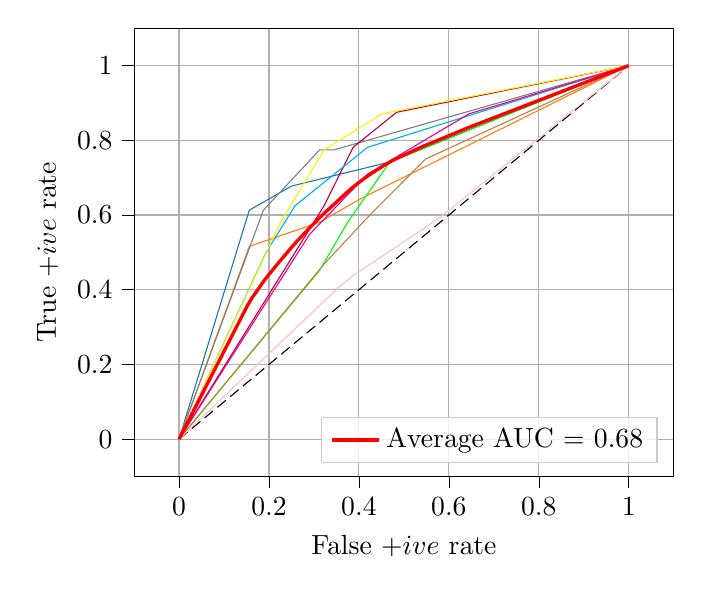
\begin{tikzpicture}
  \begin{axis}
    [
    ylabel={True $+ive$ rate},
    xlabel={False $+ive$ rate},
    tick align=outside,
    tick pos=left,
    ytick style={color=black},
    xtick style={color=black},
    grid style={gridgrey},
    xmajorgrids,
    ymajorgrids,
    legend cell align={left},
    legend columns=1,
    legend style={
      fill opacity=0.8,
      draw opacity=1,
      text opacity=1,
      at={(0.97,0.03)},
      anchor=south east,
      draw=legendgray,
    },
    ]

    \addplot[black, dashed, dash pattern=on 4pt off 2pt, forget plot] table {
      0 0
      1 1
    };


    \addplot[thin, color=steelblue, forget plot] table {
      0.0 0.0
      0.15625 0.6129032258064516
      0.25 0.6774193548387096
      0.46875 0.7419354838709677
      1.0 1.0
    };


    \addplot[thin, color=darkorange, forget plot] table {
      0.0 0.0
      0.15625 0.5161290322580645
      0.3125 0.5806451612903226
      0.40625 0.6451612903225806
      1.0 1.0
    };


    \addplot[thin, color=green, forget plot] table {
      0.0 0.0
      0.3125 0.45161290322580644
      0.375 0.5806451612903226
      0.46875 0.7419354838709677
      1.0 1.0
    };


    \addplot[thin, color=gray, forget plot] table {
      0.0 0.0
      0.1875 0.6129032258064516
      0.3125 0.7741935483870968
      0.34375 0.7741935483870968
      1.0 1.0
    };


    \addplot[thin, color=purple, forget plot] table {
      0.0 0.0
      0.3225806451612903 0.625
      0.3870967741935484 0.78125
      0.4838709677419355 0.875
      1.0 1.0
    };


    \addplot[thin, color=brown, forget plot] table {
      0.0 0.0
      0.3225806451612903 0.46875
      0.41935483870967744 0.59375
      0.5483870967741935 0.75
      1.0 1.0
    };


    \addplot[thin, color=pink, forget plot] table {
      0.0 0.0
      0.3548387096774194 0.40625
      0.3870967741935484 0.4375
      0.5806451612903226 0.59375
      1.0 1.0
    };


    \addplot[thin, color=cyan, forget plot] table {
      0.0 0.0
      0.1935483870967742 0.5
      0.25806451612903225 0.625
      0.41935483870967744 0.78125
      1.0 1.0
    };


    \addplot[thin, color=magenta, forget plot] table {
      0.0 0.0
      0.2903225806451613 0.5483870967741935
      0.41935483870967744 0.7096774193548387
      0.6451612903225806 0.8709677419354839
      1.0 1.0
    };


    \addplot[thin, color=yellow, forget plot] table {
      0.0 0.0
      0.22580645161290322 0.5806451612903226
      0.3225806451612903 0.7741935483870968
      0.45161290322580644 0.8709677419354839
      1.0 1.0
    };

    \addlegendentry{Average AUC = $0.68$}
    \addplot[very thick, red] table {
      0 0
      0.0 0.0
      0.010101010101010102 0.023756512225781533
      0.020202020202020204 0.047513024451563066
      0.030303030303030304 0.0712695366773446
      0.04040404040404041 0.09502604890312613
      0.05050505050505051 0.11878256112890768
      0.06060606060606061 0.1425390733546892
      0.07070707070707072 0.16629558558047075
      0.08080808080808081 0.19005209780625226
      0.09090909090909091 0.21380861003203377
      0.10101010101010102 0.23756512225781537
      0.11111111111111112 0.2613216344835968
      0.12121212121212122 0.2850781467093784
      0.13131313131313133 0.30883465893515993
      0.14141414141414144 0.3325911711609415
      0.15151515151515152 0.35634768338672296
      0.16161616161616163 0.3768175658742619
      0.17171717171717174 0.3943874809457043
      0.18181818181818182 0.41195739601714665
      0.19191919191919193 0.4286529763432867
      0.20202020202020204 0.44367727394975687
      0.21212121212121213 0.45859635270100824
      0.22222222222222224 0.47351543145225944
      0.23232323232323235 0.488062122734349
      0.24242424242424243 0.5024040009083998
      0.25252525252525254 0.5166465757573407
      0.26262626262626265 0.5301493214390331
      0.27272727272727276 0.5431154509591093
      0.2828282828282829 0.5560815804791857
      0.29292929292929293 0.5688811700477755
      0.30303030303030304 0.5812019572558429
      0.31313131313131315 0.5934977634711871
      0.32323232323232326 0.6053584388078523
      0.33333333333333337 0.616343082320905
      0.3434343434343435 0.6273277258339575
      0.3535353535353536 0.6386490696837106
      0.36363636363636365 0.6498263161569613
      0.37373737373737376 0.6609806057890735
      0.38383838383838387 0.6718307789880371
      0.393939393939394 0.6815327090024671
      0.4040404040404041 0.6907085447408028
      0.4141414141414142 0.6998129245502972
      0.42424242424242425 0.708306652837903
      0.43434343434343436 0.7161703610062411
      0.4444444444444445 0.7240340691745792
      0.4545454545454546 0.731746837201465
      0.4646464646464647 0.7390906404381334
      0.4747474747474748 0.7458084128779934
      0.48484848484848486 0.7520268257296058
      0.494949494949495 0.7575823597933398
      0.5050505050505051 0.7631378938570734
      0.5151515151515152 0.7686934279208073
      0.5252525252525253 0.7742489619845412
      0.5353535353535354 0.779804496048275
      0.5454545454545455 0.7853600301120087
      0.5555555555555556 0.7904443340170125
      0.5656565656565657 0.7953358619479901
      0.5757575757575758 0.800227389878968
      0.5858585858585859 0.8052030928941205
      0.595959595959596 0.8102577100506874
      0.6060606060606061 0.8153123272072543
      0.6161616161616162 0.8203669443638214
      0.6262626262626263 0.8254215615203883
      0.6363636363636365 0.8304761786769553
      0.6464646464646465 0.835485093735034
      0.6565656565656566 0.8401855196283188
      0.6666666666666667 0.8448859455216036
      0.6767676767676768 0.8495863714148884
      0.686868686868687 0.854286797308173
      0.696969696969697 0.8589872232014578
      0.7070707070707072 0.8636876490947426
      0.7171717171717172 0.8683880749880274
      0.7272727272727273 0.873088500881312
      0.7373737373737375 0.8777889267745967
      0.7474747474747475 0.8824893526678815
      0.7575757575757577 0.8871897785611663
      0.7676767676767677 0.891890204454451
      0.7777777777777778 0.8965906303477358
      0.787878787878788 0.9012910562410203
      0.797979797979798 0.9059914821343051
      0.8080808080808082 0.9106919080275901
      0.8181818181818182 0.9153923339208745
      0.8282828282828284 0.9200927598141595
      0.8383838383838385 0.9247931857074441
      0.8484848484848485 0.9294936116007289
      0.8585858585858587 0.9341940374940136
      0.8686868686868687 0.9388944633872984
      0.8787878787878789 0.9435948892805829
      0.888888888888889 0.948295315173868
      0.8989898989898991 0.9529957410671528
      0.9090909090909092 0.9576961669604375
      0.9191919191919192 0.9623965928537223
      0.9292929292929294 0.9670970187470068
      0.9393939393939394 0.9717974446402916
      0.9494949494949496 0.9764978705335764
      0.9595959595959597 0.9811982964268611
      0.9696969696969697 0.9858987223201456
      0.9797979797979799 0.9905991482134308
      0.98989898989899 0.9952995741067152
      1.0 1.0
    };


  \end{axis}
\end{tikzpicture}
}
              \captionsetup{justification=centering}
              \caption{Without data leak}
            \end{subfigure}
            \caption{PseU-ST results on \textbf{S\_628} dataset}\label{fig:pseu-st_s628}
        \end{figure}

        \begin{figure}[H]
            \centering
            \begin{subfigure}{0.45\textwidth}
              \centering
              \resizebox{\textwidth}{!}{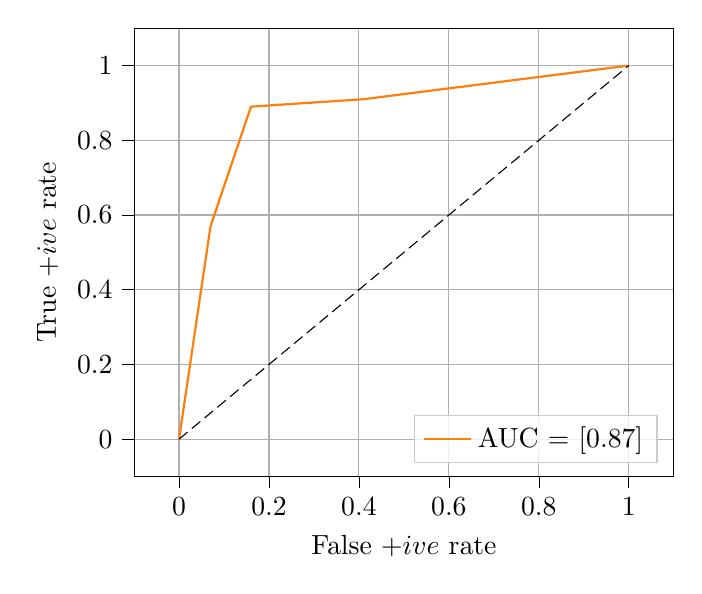
\begin{tikzpicture}
  \begin{axis}
    [
    ylabel={True $+ive$ rate},
    xlabel={False $+ive$ rate},
    tick align=outside,
    tick pos=left,
    ytick style={color=black},
    xtick style={color=black},
    grid style={gridgrey},
    xmajorgrids,
    ymajorgrids,
    legend cell align={left},
    legend columns=1,
    legend style={
      fill opacity=0.8,
      draw opacity=1,
      text opacity=1,
      at={(0.97,0.03)},
      anchor=south east,
      draw=legendgray,
    },
    ]
    \addlegendentry{AUC = $[0.87]$}
    \addplot[thick, darkorange] table {
      0.0 0.0
      0.07 0.57
      0.16 0.89
      0.41 0.91
      1.0 1.0
    };
    \addplot[black, dashed, dash pattern=on 4pt off 2pt] table {
      0 0
      1 1
    };
  \end{axis}
\end{tikzpicture}
}
              \captionsetup{justification=centering}
              \caption{With data leak}
            \end{subfigure}%
            \hspace{0.05\textwidth}
            \begin{subfigure}{0.45\textwidth}
              \centering
              \resizebox{\textwidth}{!}{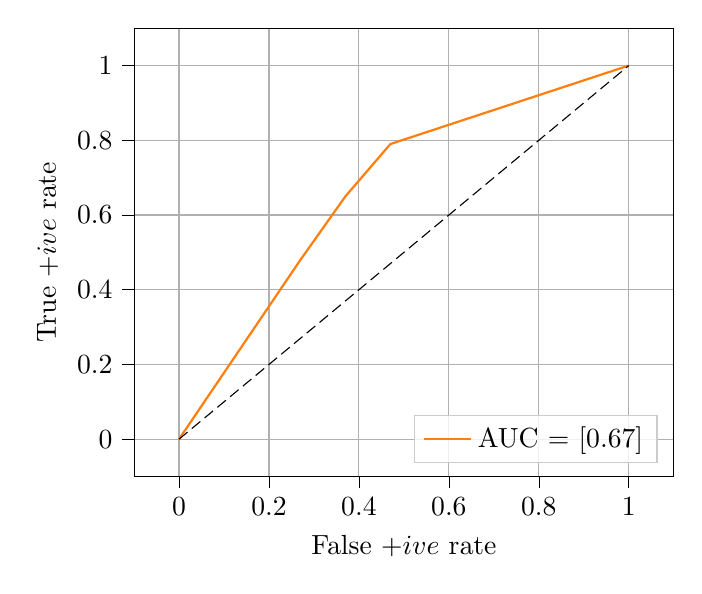
\begin{tikzpicture}
  \begin{axis}
    [
    ylabel={True $+ive$ rate},
    xlabel={False $+ive$ rate},
    tick align=outside,
    tick pos=left,
    ytick style={color=black},
    xtick style={color=black},
    grid style={gridgrey},
    xmajorgrids,
    ymajorgrids,
    legend cell align={left},
    legend columns=1,
    legend style={
      fill opacity=0.8,
      draw opacity=1,
      text opacity=1,
      at={(0.97,0.03)},
      anchor=south east,
      draw=legendgray,
    },
    ]
    \addlegendentry{AUC = $[0.67]$}
    \addplot[thick, darkorange] table {
      0.0 0.0
      0.27 0.48
      0.37 0.65
      0.47 0.79
      1.0 1.0
    };
    \addplot[black, dashed, dash pattern=on 4pt off 2pt] table {
      0 0
      1 1
    };
  \end{axis}
\end{tikzpicture}
}
              \captionsetup{justification=centering}
              \caption{Without data leak}
            \end{subfigure}
            \caption{PseU-ST results on \textbf{S\_200} dataset}\label{fig:pseu-st_s200}
        \end{figure}

      \paragraph{Mus musculus}
        \noindent
        \begin{table}[H]
            \centering
            \begin{tabular}{lcc}
              \toprule
              \textbf{Metric} & \textbf{Original} & \textbf{Fixed} \\
              \midrule
              Accuracy        & 90\%              & 67\%           \\
              MCC             & 0.79              & 0.35           \\
              Sensitivity     & 91\%              & 68\%           \\
              Specificity     & 89\%              & 67\%           \\
              \bottomrule
            \end{tabular}
            \caption{Results for M\_944 dataset}
            \label{tab:pseu-st_pstnpss_mm}
        \end{table}

        \begin{figure}[H]
            \centering
            \begin{subfigure}{0.47\textwidth}
              \centering
              \resizebox{\textwidth}{!}{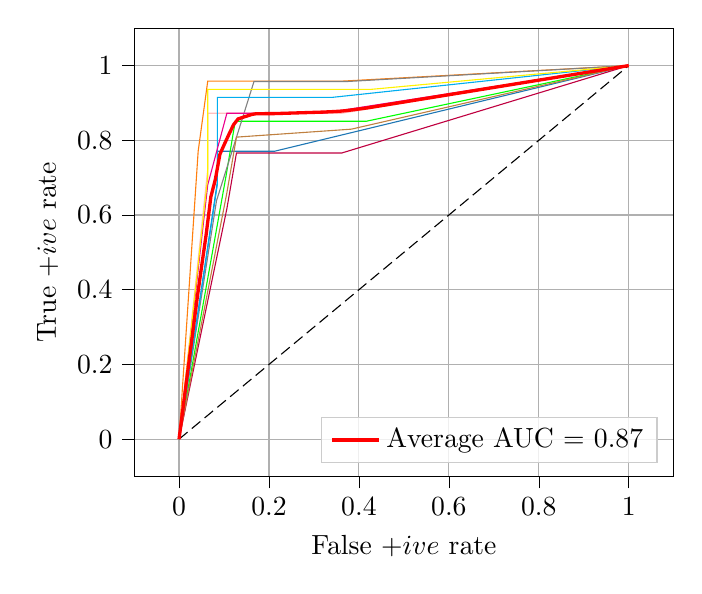
\begin{tikzpicture}
  \begin{axis}
    [
    ylabel={True $+ive$ rate},
    xlabel={False $+ive$ rate},
    tick align=outside,
    tick pos=left,
    ytick style={color=black},
    xtick style={color=black},
    grid style={gridgrey},
    xmajorgrids,
    ymajorgrids,
    legend cell align={left},
    legend columns=1,
    legend style={
      fill opacity=0.8,
      draw opacity=1,
      text opacity=1,
      at={(0.97,0.03)},
      anchor=south east,
      draw=legendgray,
    },
    ]

    \addplot[black, dashed, dash pattern=on 4pt off 2pt, forget plot] table {
      0 0
      1 1
    };


    \addplot[thin, color=steelblue, forget plot] table {
      0.0 0.0
      0.0851063829787234 0.6875
      0.0851063829787234 0.7708333333333334
      0.2127659574468085 0.7708333333333334
      1.0 1.0
    };


    \addplot[thin, color=darkorange, forget plot] table {
      0.0 0.0
      0.0425531914893617 0.7708333333333334
      0.06382978723404255 0.9583333333333334
      0.3617021276595745 0.9583333333333334
      1.0 1.0
    };


    \addplot[thin, color=green, forget plot] table {
      0.0 0.0
      0.10416666666666667 0.7021276595744681
      0.125 0.851063829787234
      0.4166666666666667 0.851063829787234
      1.0 1.0
    };


    \addplot[thin, color=gray, forget plot] table {
      0.0 0.0
      0.08333333333333333 0.6382978723404256
      0.16666666666666666 0.9574468085106383
      0.375 0.9574468085106383
      1.0 1.0
    };


    \addplot[thin, color=purple, forget plot] table {
      0.0 0.0
      0.10638297872340426 0.6170212765957447
      0.1276595744680851 0.7659574468085106
      0.3617021276595745 0.7659574468085106
      1.0 1.0
    };


    \addplot[thin, color=brown, forget plot] table {
      0.0 0.0
      0.10638297872340426 0.6595744680851063
      0.1276595744680851 0.8085106382978723
      0.3829787234042553 0.8297872340425532
      1.0 1.0
    };


    \addplot[thin, color=pink, forget plot] table {
      0.0 0.0
      0.06382978723404255 0.723404255319149
      0.06382978723404255 0.8723404255319149
      0.3617021276595745 0.8723404255319149
      1.0 1.0
    };


    \addplot[thin, color=cyan, forget plot] table {
      0.0 0.0
      0.0851063829787234 0.6808510638297872
      0.0851063829787234 0.9148936170212766
      0.3404255319148936 0.9148936170212766
      1.0 1.0
    };


    \addplot[thin, color=magenta, forget plot] table {
      0.0 0.0
      0.06382978723404255 0.6808510638297872
      0.10638297872340426 0.8723404255319149
      0.3191489361702128 0.8723404255319149
      1.0 1.0
    };


    \addplot[thin, color=yellow, forget plot] table {
      0.0 0.0
      0.06382978723404255 0.7021276595744681
      0.06382978723404255 0.9361702127659575
      0.425531914893617 0.9361702127659575
      1.0 1.0
    };

    \addlegendentry{Average AUC = $0.87$}
    \addplot[very thick, red] table {
      0 0
      0.0 0.0
      0.010101010101010102 0.09453808922558923
      0.020202020202020204 0.18907617845117847
      0.030303030303030304 0.28361426767676773
      0.04040404040404041 0.37815235690235693
      0.05050505050505051 0.46529356060606064
      0.06060606060606061 0.550435606060606
      0.07070707070707072 0.6482146598968408
      0.08080808080808081 0.6956673114119922
      0.09090909090909091 0.7626265312701483
      0.10101010101010102 0.7899701805286913
      0.11111111111111112 0.8164154846335698
      0.12121212121212122 0.8416465183752418
      0.13131313131313133 0.8572798015617165
      0.14141414141414144 0.8612324485994698
      0.15151515151515152 0.8651850956372232
      0.16161616161616163 0.8691377426749767
      0.17171717171717174 0.871156153735941
      0.18181818181818182 0.871240328820116
      0.19191919191919193 0.8713245039042912
      0.20202020202020204 0.8714086789884663
      0.21212121212121213 0.8714928540726413
      0.22222222222222224 0.8718523044320918
      0.23232323232323235 0.8722305235603109
      0.24242424242424243 0.8726087426885301
      0.25252525252525254 0.8729869618167492
      0.26262626262626265 0.8733651809449683
      0.27272727272727276 0.8737434000731874
      0.2828282828282829 0.8741216192014065
      0.29292929292929293 0.8744998383296256
      0.30303030303030304 0.8748780574578447
      0.31313131313131315 0.8752562765860639
      0.32323232323232326 0.8757110592216975
      0.33333333333333337 0.8762786722893108
      0.3434343434343435 0.8768851087313682
      0.3535353535353536 0.8775830574131878
      0.36363636363636365 0.8784032390629852
      0.37373737373737376 0.879739515466466
      0.38383838383838387 0.8811525190339811
      0.393939393939394 0.8827520417425276
      0.4040404040404041 0.8843515644510742
      0.4141414141414142 0.8859510871596207
      0.42424242424242425 0.8877440334658463
      0.43434343434343436 0.8896993600762958
      0.4444444444444445 0.8916690143606478
      0.4545454545454546 0.8936386686449996
      0.4646464646464647 0.8956083229293513
      0.4747474747474748 0.8975779772137035
      0.48484848484848486 0.8995476314980552
      0.494949494949495 0.901517285782407
      0.5050505050505051 0.9034869400667589
      0.5151515151515152 0.9054565943511108
      0.5252525252525253 0.9074262486354627
      0.5353535353535354 0.9093959029198142
      0.5454545454545455 0.9113655572041663
      0.5555555555555556 0.913335211488518
      0.5656565656565657 0.91530486577287
      0.5757575757575758 0.9172745200572219
      0.5858585858585859 0.9192441743415738
      0.595959595959596 0.9212138286259256
      0.6060606060606061 0.9231834829102775
      0.6161616161616162 0.9251531371946294
      0.6262626262626263 0.9271227914789811
      0.6363636363636365 0.929092445763333
      0.6464646464646465 0.931062100047685
      0.6565656565656566 0.9330317543320368
      0.6666666666666667 0.9350014086163887
      0.6767676767676768 0.9369710629007404
      0.686868686868687 0.9389407171850923
      0.696969696969697 0.9409103714694442
      0.7070707070707072 0.9428800257537961
      0.7171717171717172 0.9448496800381478
      0.7272727272727273 0.9468193343225
      0.7373737373737375 0.9487889886068517
      0.7474747474747475 0.9507586428912035
      0.7575757575757577 0.9527282971755552
      0.7676767676767677 0.9546979514599073
      0.7777777777777778 0.956667605744259
      0.787878787878788 0.9586372600286109
      0.797979797979798 0.9606069143129629
      0.8080808080808082 0.9625765685973148
      0.8181818181818182 0.9645462228816666
      0.8282828282828284 0.9665158771660185
      0.8383838383838385 0.9684855314503702
      0.8484848484848485 0.9704551857347221
      0.8585858585858587 0.972424840019074
      0.8686868686868687 0.9743944943034257
      0.8787878787878789 0.9763641485877776
      0.888888888888889 0.9783338028721296
      0.8989898989898991 0.9803034571564814
      0.9090909090909092 0.9822731114408331
      0.9191919191919192 0.984242765725185
      0.9292929292929294 0.9862124200095369
      0.9393939393939394 0.9881820742938888
      0.9494949494949496 0.9901517285782406
      0.9595959595959597 0.9921213828625925
      0.9696969696969697 0.9940910371469445
      0.9797979797979799 0.9960606914312964
      0.98989898989899 0.9980303457156483
      1.0 1.0
    };


  \end{axis}
\end{tikzpicture}
}
              \captionsetup{justification=centering}
              \caption{With data leak}
            \end{subfigure}%
            \hspace{0.05\textwidth}
            \begin{subfigure}{0.47\textwidth}
              \centering
              \resizebox{\textwidth}{!}{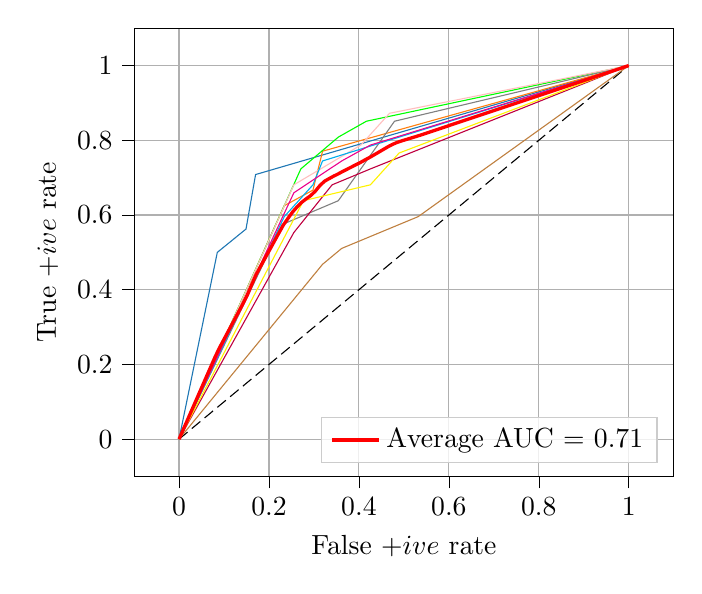
\begin{tikzpicture}
  \begin{axis}
    [
    ylabel={True $+ive$ rate},
    xlabel={False $+ive$ rate},
    tick align=outside,
    tick pos=left,
    ytick style={color=black},
    xtick style={color=black},
    grid style={gridgrey},
    xmajorgrids,
    ymajorgrids,
    legend cell align={left},
    legend columns=1,
    legend style={
      fill opacity=0.8,
      draw opacity=1,
      text opacity=1,
      at={(0.97,0.03)},
      anchor=south east,
      draw=legendgray,
    },
    ]

    \addplot[black, dashed, dash pattern=on 4pt off 2pt, forget plot] table {
      0 0
      1 1
    };


    \addplot[thin, color=steelblue, forget plot] table {
      0.0 0.0
      0.0851063829787234 0.5
      0.14893617021276595 0.5625
      0.1702127659574468 0.7083333333333334
      1.0 1.0
    };


    \addplot[thin, color=darkorange, forget plot] table {
      0.0 0.0
      0.23404255319148937 0.625
      0.2978723404255319 0.6666666666666666
      0.3191489361702128 0.7708333333333334
      1.0 1.0
    };


    \addplot[thin, color=green, forget plot] table {
      0.0 0.0
      0.2708333333333333 0.723404255319149
      0.3541666666666667 0.8085106382978723
      0.4166666666666667 0.851063829787234
      1.0 1.0
    };


    \addplot[thin, color=gray, forget plot] table {
      0.0 0.0
      0.22916666666666666 0.574468085106383
      0.3541666666666667 0.6382978723404256
      0.4791666666666667 0.851063829787234
      1.0 1.0
    };


    \addplot[thin, color=purple, forget plot] table {
      0.0 0.0
      0.2553191489361702 0.5531914893617021
      0.3404255319148936 0.6808510638297872
      0.425531914893617 0.723404255319149
      1.0 1.0
    };


    \addplot[thin, color=brown, forget plot] table {
      0.0 0.0
      0.3191489361702128 0.46808510638297873
      0.3617021276595745 0.5106382978723404
      0.5319148936170213 0.5957446808510638
      1.0 1.0
    };


    \addplot[thin, color=pink, forget plot] table {
      0.0 0.0
      0.2553191489361702 0.6808510638297872
      0.40425531914893614 0.7872340425531915
      0.46808510638297873 0.8723404255319149
      1.0 1.0
    };


    \addplot[thin, color=cyan, forget plot] table {
      0.0 0.0
      0.23404255319148937 0.5957446808510638
      0.2978723404255319 0.6808510638297872
      0.3191489361702128 0.7446808510638298
      1.0 1.0
    };


    \addplot[thin, color=magenta, forget plot] table {
      0.0 0.0
      0.2553191489361702 0.6595744680851063
      0.3617021276595745 0.7446808510638298
      0.425531914893617 0.7872340425531915
      1.0 1.0
    };


    \addplot[thin, color=yellow, forget plot] table {
      0.0 0.0
      0.2765957446808511 0.6382978723404256
      0.425531914893617 0.6808510638297872
      0.48936170212765956 0.7659574468085106
      1.0 1.0
    };

    \addlegendentry{Average AUC = $0.71$}
    \addplot[very thick, red] table {
      0 0
      0.0 0.0
      0.010101010101010102 0.027737106721632838
      0.020202020202020204 0.055474213443265676
      0.030303030303030304 0.08321132016489849
      0.04040404040404041 0.11094842688653135
      0.05050505050505051 0.13868553360816419
      0.06060606060606061 0.16642264032979698
      0.07070707070707072 0.19415974705142985
      0.08080808080808081 0.2218968537730627
      0.09090909090909091 0.24679305140378646
      0.10101010101010102 0.2695848719301331
      0.11111111111111112 0.29237669245647974
      0.12121212121212122 0.31516851298282633
      0.13131313131313133 0.33796033350917304
      0.14141414141414144 0.36075215403551963
      0.15151515151515152 0.38505912607701775
      0.16161616161616163 0.4137852900377079
      0.17171717171717174 0.4415331884367991
      0.18181818181818182 0.46369099791246804
      0.19191919191919193 0.48584880738813696
      0.20202020202020204 0.5080066168638059
      0.21212121212121213 0.5301644263394747
      0.22222222222222224 0.5523222358151436
      0.23232323232323235 0.5738499532680708
      0.24242424242424243 0.5912843519758413
      0.25252525252525254 0.60816344477692
      0.26262626262626265 0.6218256677653841
      0.27272727272727276 0.6339454576156703
      0.2828282828282829 0.6434510767666797
      0.29292929292929293 0.6521744993908115
      0.30303030303030304 0.6639461346376241
      0.31313131313131315 0.678638973647839
      0.32323232323232326 0.6902076493718228
      0.33333333333333337 0.6971722949897818
      0.3434343434343435 0.7038360594557956
      0.3535353535353536 0.7097906040636538
      0.36363636363636365 0.7164285787166439
      0.37373737373737376 0.7226030531188998
      0.38383838383838387 0.7287775275211557
      0.393939393939394 0.7349520019234116
      0.4040404040404041 0.7411264763256673
      0.4141414141414142 0.7479129470846005
      0.42424242424242425 0.7543903494493589
      0.43434343434343436 0.7614060061348773
      0.4444444444444445 0.7685161572411314
      0.4545454545454546 0.7756263083473854
      0.4646464646464647 0.7827364594536396
      0.4747474747474748 0.7891181916187089
      0.48484848484848486 0.7943193234542415
      0.494949494949495 0.798405690621818
      0.5050505050505051 0.8020971512774666
      0.5151515151515152 0.8057886119331155
      0.5252525252525253 0.8094800725887643
      0.5353535353535354 0.8132965747621045
      0.5454545454545455 0.8173553448759717
      0.5555555555555556 0.8214141149898389
      0.5656565656565657 0.8254728851037063
      0.5757575757575758 0.8295316552175738
      0.5858585858585859 0.8335904253314409
      0.595959595959596 0.8376491954453081
      0.6060606060606061 0.8417079655591755
      0.6161616161616162 0.845766735673043
      0.6262626262626263 0.8498255057869102
      0.6363636363636365 0.8538842759007773
      0.6464646464646465 0.8579430460146446
      0.6565656565656566 0.862001816128512
      0.6666666666666667 0.8660605862423794
      0.6767676767676768 0.8701193563562466
      0.686868686868687 0.8741781264701138
      0.696969696969697 0.8782368965839812
      0.7070707070707072 0.8822956666978484
      0.7171717171717172 0.8863544368117158
      0.7272727272727273 0.890413206925583
      0.7373737373737375 0.8944719770394503
      0.7474747474747475 0.8985307471533176
      0.7575757575757577 0.9025895172671851
      0.7676767676767677 0.9066482873810523
      0.7777777777777778 0.9107070574949196
      0.787878787878788 0.9147658276087869
      0.797979797979798 0.918824597722654
      0.8080808080808082 0.9228833678365213
      0.8181818181818182 0.9269421379503887
      0.8282828282828284 0.9310009080642561
      0.8383838383838385 0.9350596781781231
      0.8484848484848485 0.9391184482919905
      0.8585858585858587 0.9431772184058579
      0.8686868686868687 0.9472359885197251
      0.8787878787878789 0.9512947586335925
      0.888888888888889 0.9553535287474599
      0.8989898989898991 0.959412298861327
      0.9090909090909092 0.9634710689751944
      0.9191919191919192 0.9675298390890618
      0.9292929292929294 0.971588609202929
      0.9393939393939394 0.9756473793167961
      0.9494949494949496 0.9797061494306636
      0.9595959595959597 0.9837649195445307
      0.9696969696969697 0.9878236896583982
      0.9797979797979799 0.9918824597722654
      0.98989898989899 0.9959412298861328
      1.0 1.0
    };


  \end{axis}
\end{tikzpicture}
}
              \captionsetup{justification=centering}
              \caption{Without data leak}
            \end{subfigure}
            \caption{PseU-ST results on \textbf{H\_944} dataset}\label{fig:pseu-st_m944}
        \end{figure}

%\section{Conclusion}
%
%The results indicate that the improper use of position-specific encodings, as seen in Porpoise and similar studies, can lead to inflated performance metrics due to data leakage and bias. After correcting the encoding process to ensure that matrices are generated using only the training samples, we observe a significant decrease in performance across all metrics, highlighting the importance of proper encoding techniques for accurate model evaluation.



  \chapter{Conclusion}\label{ch:conclusion}
    In this study, we addressed the problem of pseudouridine (Ψ) prediction using machine learning (ML) and deep learning (DL) techniques. Through an extensive review of recent literature, covering approximately all the papers, we identified that several approaches adopted by existing studies contained fundamental flaws in their methodologies, particularly in terms of how encodings were applied. To substantiate this, we performed data exploratory analysis (DEA) to check the correlation between features within the datasets, and re-evaluated the techniques from previous studies using more accurate encoding schemes. Our findings highlighted a critical issue: many of the datasets lacked significant correlation, making it challenging to classify Ψ sites with high accuracy.

    One of the key problems identified is that the datasets used in prior research predominantly rely on small sequences (typically 21 nucleotides) that fail to provide sufficient contextual information for accurate predictions. This limits the ability of models to generalize effectively. Furthermore, we noted that only the positive samples (i.e., Ψ-modified sequences) in the datasets are clinically verified, while the negative samples (non-Ψ sequences) are not. This raises concerns about the reliability of these negative samples, as some may, in fact, be positive but untested, thus introducing noise into the classification process.

    Additionally, our analysis pointed out that in real-world scenarios, sequences with unmodified U at the center may exist, even if the probability is low. By increasing the window size (e.g., to 31 or 41 nucleotides), we could capture more contextual information, potentially reducing the likelihood of false negatives. However, current sequence and dataset sizes remain too small for sequential models, such as Transformers or other deep learning-based architectures, to generalize effectively, which prevents their practical application in this domain.

    Another significant observation came from comparing our results with nanopore sequencing, which provides additional layers of information (beyond nucleotide sequences) that are crucial for identifying Ψ sites. The discrepancy between ML/DL predictions and nanopore results underscores the limitations of current datasets and encoding approaches.


    \section{Future work}\label{sec:future-work}

      For future work, several improvements can be pursued. First, creating larger datasets with longer sequences and ensuring that both positive and negative samples are clinically tested or species-specific will be critical to improving prediction accuracy. Additionally, incorporating sequences from other RNA modification datasets, where U is known to remain unmodified, could enhance the quality of the negative samples. Another promising direction involves augmenting the datasets with advanced techniques, such as Gaussian Mixture Models (GMMs) or Variational Autoencoders (VAEs), to generate synthetic samples and expand the training data.

      Furthermore, applying sequential models to larger, more comprehensive datasets could enable a more robust analysis of Ψ site prediction. Another alternative would be exploring Kernel-based Attention Networks (KANs), which have shown promising results on highly non-linear data. Given the non-linear nature of pseudouridine modification as observed in our DEA, KANs might offer a viable path forward.

      In conclusion, while pseudouridine prediction remains a challenging problem due to inherent limitations in dataset quality and size, addressing these issues through better dataset construction, augmentation, and advanced modeling techniques holds the potential to significantly improve prediction performance.


    \section{Resources \& Materials}\label{sec:resources-&-materials}
      All the resources are generated through source code and that source code can be accessed from \url{https://github.com/ArishSultan/https://github.com/ArishSultan/rna_modification.git}


% Bibliography
      \bibliography{references}
\end{document}
